\documentclass[twoside]{book}

% Packages required by doxygen
\usepackage{fixltx2e}
\usepackage{calc}
\usepackage{doxygen}
\usepackage[export]{adjustbox} % also loads graphicx
\usepackage{graphicx}
\usepackage[utf8]{inputenc}
\usepackage{makeidx}
\usepackage{multicol}
\usepackage{multirow}
\PassOptionsToPackage{warn}{textcomp}
\usepackage{textcomp}
\usepackage[nointegrals]{wasysym}
\usepackage[table]{xcolor}

% Font selection
\usepackage[T1]{fontenc}
\usepackage[scaled=.90]{helvet}
\usepackage{courier}
\usepackage{amssymb}
\usepackage{sectsty}
\renewcommand{\familydefault}{\sfdefault}
\allsectionsfont{%
  \fontseries{bc}\selectfont%
  \color{darkgray}%
}
\renewcommand{\DoxyLabelFont}{%
  \fontseries{bc}\selectfont%
  \color{darkgray}%
}
\newcommand{\+}{\discretionary{\mbox{\scriptsize$\hookleftarrow$}}{}{}}

% Page & text layout
\usepackage{geometry}
\geometry{%
  letterpaper,%
  top=2.5cm,%
  bottom=2.5cm,%
  left=2.5cm,%
  right=2.5cm%
}
\tolerance=750
\hfuzz=15pt
\hbadness=750
\setlength{\emergencystretch}{15pt}
\setlength{\parindent}{0cm}
\setlength{\parskip}{0.2cm}
\makeatletter
\renewcommand{\paragraph}{%
  \@startsection{paragraph}{4}{0ex}{-1.0ex}{1.0ex}{%
    \normalfont\normalsize\bfseries\SS@parafont%
  }%
}
\renewcommand{\subparagraph}{%
  \@startsection{subparagraph}{5}{0ex}{-1.0ex}{1.0ex}{%
    \normalfont\normalsize\bfseries\SS@subparafont%
  }%
}
\makeatother

% Headers & footers
\usepackage{fancyhdr}
\pagestyle{fancyplain}
\fancyhead[LE]{\fancyplain{}{\bfseries\thepage}}
\fancyhead[CE]{\fancyplain{}{}}
\fancyhead[RE]{\fancyplain{}{\bfseries\leftmark}}
\fancyhead[LO]{\fancyplain{}{\bfseries\rightmark}}
\fancyhead[CO]{\fancyplain{}{}}
\fancyhead[RO]{\fancyplain{}{\bfseries\thepage}}
\fancyfoot[LE]{\fancyplain{}{}}
\fancyfoot[CE]{\fancyplain{}{}}
\fancyfoot[RE]{\fancyplain{}{\bfseries\scriptsize Generated on Tue Jul 31 2018 17\+:58\+:25 for Genetic Technology Mapping by Doxygen }}
\fancyfoot[LO]{\fancyplain{}{\bfseries\scriptsize Generated on Tue Jul 31 2018 17\+:58\+:25 for Genetic Technology Mapping by Doxygen }}
\fancyfoot[CO]{\fancyplain{}{}}
\fancyfoot[RO]{\fancyplain{}{}}
\renewcommand{\footrulewidth}{0.4pt}
\renewcommand{\chaptermark}[1]{%
  \markboth{#1}{}%
}
\renewcommand{\sectionmark}[1]{%
  \markright{\thesection\ #1}%
}

% Indices & bibliography
\usepackage{natbib}
\usepackage[titles]{tocloft}
\setcounter{tocdepth}{3}
\setcounter{secnumdepth}{5}
\makeindex

% Hyperlinks (required, but should be loaded last)
\usepackage{ifpdf}
\ifpdf
  \usepackage[pdftex,pagebackref=true]{hyperref}
\else
  \usepackage[ps2pdf,pagebackref=true]{hyperref}
\fi
\hypersetup{%
  colorlinks=true,%
  linkcolor=blue,%
  citecolor=blue,%
  unicode%
}

% Custom commands
\newcommand{\clearemptydoublepage}{%
  \newpage{\pagestyle{empty}\cleardoublepage}%
}


%===== C O N T E N T S =====

\begin{document}

% Titlepage & ToC
\hypersetup{pageanchor=false,
             bookmarks=true,
             bookmarksnumbered=true,
             pdfencoding=unicode
            }
\pagenumbering{roman}
\begin{titlepage}
\vspace*{7cm}
\begin{center}%
{\Large Genetic Technology Mapping \\[1ex]\large 1.\+0 }\\
\vspace*{1cm}
{\large Generated by Doxygen 1.8.9.1}\\
\vspace*{0.5cm}
{\small Tue Jul 31 2018 17:58:25}\\
\end{center}
\end{titlepage}
\clearemptydoublepage
\tableofcontents
\clearemptydoublepage
\pagenumbering{arabic}
\hypersetup{pageanchor=true}

%--- Begin generated contents ---
\chapter{2018-\/wannabe-\/postdoc-\/1}
\label{md_README}
\hypertarget{md_README}{}
This is the repository for problem 1 of the 2018 B\+D\+Athlon programming contest.

It my solution for the problem on genetic technology mapping.

\subsection*{Organization of the Repository}


\begin{DoxyItemize}
\item docs
\begin{DoxyItemize}
\item Documentation generated by documentation generators
\begin{DoxyItemize}
\item Doxygen
\item pydoc (for Python scripts)\+: /usr/bin/pydoc
\end{DoxyItemize}
\end{DoxyItemize}
\item notes
\begin{DoxyItemize}
\item Software licenses
\begin{DoxyItemize}
\item {\itshape M\+I\+T License}.
\end{DoxyItemize}
\item Guidelines for collaborating on open source software and/or hardware projects.
\item Documentation about guidelines that I am following for my research, and for my research collaborators to know about.
\end{DoxyItemize}
\end{DoxyItemize}

Externalities list.
\begin{DoxyItemize}
\item {\itshape Publicly available library, A\+P\+I, or framework} that I have used as external components for my software.
\begin{DoxyItemize}
\item Some {\itshape Python} modules from the repository \href{https://github.com/eda-ricercatore/bibtex-analytics}{\tt bibtex-\/analytics}, which I developed.
\end{DoxyItemize}
\end{DoxyItemize}

\subsection*{Description of the Software Solution for Genetic Technology Mapping}

My solution for genetic technology mapping, {\bfseries problem1\+\_\+solution.\+py}, takes in two input parameters, $\ast$$\ast$\mbox{[}input J\+S\+O\+N netlist\mbox{]}$\ast$$\ast$ and $\ast$$\ast$\mbox{[}output J\+S\+O\+N technology mapping\mbox{]}$\ast$$\ast$.

The first input parameter $\ast$$\ast$\mbox{[}input J\+S\+O\+N netlist\mbox{]}$\ast$$\ast$ is a J\+S\+O\+N file that contains a structural netlist for genetic technology mapping.

The other input parameter $\ast$$\ast$\mbox{[}output J\+S\+O\+N technology mapping\mbox{]}$\ast$$\ast$ is the filename of an output J\+S\+O\+N file that contains a genetic technology mapping for the input structural netlist ($\ast$$\ast$\mbox{[}input J\+S\+O\+N netlist\mbox{]}$\ast$$\ast$).

The front-\/end of {\bfseries problem1\+\_\+solution.\+py} parses the input arguments, checks their validity, and parses the input structural netlist for genetic technology mapping. It also parses the genetic technology library {\bfseries genetic\+\_\+gate\+\_\+library.\+json}, maps each genetic N\+O\+T gate into a {\itshape genetic\+\_\+not\+\_\+gate} object, and stores each object in a map of $\ast$(id,objects)$\ast$; the {\itshape id} of the object is the {\itshape id} field of the genetic N\+O\+T gate, which is specified in the genetic technology library.

The genetic technology mapping engine of {\bfseries problem1\+\_\+solution.\+py} consists of a (set of) solution(s) to perform genetic technology mapping. A solution is an implementation of a known/new algorithm/heuristic for genetic technology mapping.

{\bfseries Dr. Nicholas Roehner and Dr. Curtis Madsen, I am running out of time, so I will sketch the outline of my solutions, and update them as I solve the problem.}

Solution {\itshape 1a} performs {\itshape brute force search} to explore different options for genetic technology mapping.
\begin{DoxyItemize}
\item Explore each permutation of N\+O\+T gates.
\item For each selection, store its alpha value and the permutation in a table
\item Enumerate a table to find the largest alpha value, and select the corresponding permutation of N\+O\+T gates.
\end{DoxyItemize}

Solution {\itshape 1b} uses simulated annealing for discrete optimization.
\begin{DoxyItemize}
\item Pseudo-\/randomly select a permutation of N\+O\+T gates.
\item Initialize temperature to be very hot
\item While temperature is not 0, cool the temperature of the annealing process.
\begin{DoxyItemize}
\item As the temperature cools, slowly decrease the
\end{DoxyItemize}
\end{DoxyItemize}

Solution {\itshape 1b} uses a genetic algorithm for discrete optimization.

Other solutions considered\+:
\begin{DoxyItemize}
\item 0-\/1 integer linear programming (I\+L\+P)
\begin{DoxyItemize}
\item Can\textquotesingle{}t formulate the objective function of the 0-\/1 I\+L\+P problem.
\end{DoxyItemize}
\item pseudo-\/boolan optimization (P\+B\+O)
\begin{DoxyItemize}
\item Can\textquotesingle{}t formulate the conjunctive normal form (C\+N\+F) boolean satisfiability formula for P\+B\+O.
\end{DoxyItemize}
\end{DoxyItemize}

The back-\/end of {\bfseries problem1\+\_\+solution.\+py} generates an output file containing the genetic technology mapping of the input genetic circuit, in J\+S\+O\+N format.

\subsection*{Instructions on How to Build and Run the Software Solution}

\subsubsection*{Building and Executing the Software Solution}

To execute the software solution, try\+: \begin{DoxyVerb}./problem1_solution.py [input JSON netlist] [output JSON technology mapping]
\end{DoxyVerb}


Input Parameters\+: \mbox{[}input J\+S\+O\+N netlist\mbox{]}\+: A J\+S\+O\+N file that contains a structural netlist for genetic technology mapping.

\mbox{[}output J\+S\+O\+N technology mapping\mbox{]}\+: A filename of an output J\+S\+O\+N file that contains a genetic technology mapping for the input structural netlist.

\subsubsection*{Documentation Generation}

To use {\itshape Doxygen} to generate documentation for the Python software, try\+: \begin{DoxyVerb}make doxygen
\end{DoxyVerb}


To view the {\itshape Doxygen}-\/generated documention, open the file \href{https://github.com/BDAthlon/2018-wannabe-postdoc-1/blob/master/docs/html/index.html}{\tt $\ast$$\ast$docs/html/index.html$\ast$$\ast$} in a Web browser.

The command {\bfseries make doxygeninit} has already been used to generate a {\itshape Doxygen} configuration file named {\bfseries doxygen.\+config}. {\bfseries D\+O N\+O\+T R\+U\+N T\+H\+E C\+O\+M\+M\+A\+N\+D {\itshape doxygen.\+config} A\+G\+A\+I\+N!!!}

To use {\itshape pydoc} to view or generate documentation for my software solution (Python code), try\+:

pydoc \mbox{[}{\itshape Python} package/module/class\mbox{]}

A {\itshape Python} package corresponds to a subdirectory of this repository, while a {\itshape Python} module/class corresponds to a {\itshape Python} source file in a subdirectory.

\subsection*{Miscellaneous}

\subsubsection*{Refactoring attempt\+: {\itshape Utilities} package}

Refactor the class {\bfseries queue\+\_\+ip\+\_\+args} in the {\itshape Python} module {\itshape \hyperlink{queue__ip__arguments_8py}{queue\+\_\+ip\+\_\+arguments.\+py}}, so that does not need the argument {\bfseries which\+\_\+script} for the static method {\bfseries set\+\_\+input\+\_\+arguments(list\+\_\+of\+\_\+ip\+\_\+arguments,which\+\_\+script)}. That is, refactor the static method to {\bfseries set\+\_\+input\+\_\+arguments(list\+\_\+of\+\_\+ip\+\_\+arguments)}.

Using this refactored {\itshape Python} class has an impact on its corresponding {\itshape Python} class in the $\ast$$\ast$\href{https://github.com/eda-ricercatore/bibtex-analytics}{\tt bibtex-\/analytics}$\ast$$\ast$ software. Use this refactored code to handle usage modes in the {\bfseries bibtex-\/analytics} software, such as\+: obtaining a sorted list of keyphrases/keywords; obtaining a sorted list of publishers, organizations, and institutions; and a list of series of books or conference proceedings. These modes shall be specified by an input argument. If multiple modes are specified as input arguments, an order of precedance is used to specify which mode shall be selected for processing. The $\ast$$\ast$\href{https://github.com/eda-ricercatore/bibtex-analytics}{\tt bibtex-\/analytics}$\ast$$\ast$ software can only process one mode per execution run.

\section*{References}

Citations/\+References that use the La\+Te\+X/\+Bib\+Te\+X notation are taken from my Bib\+Te\+X database (set of Bib\+Te\+X entries).

Additional references not found in the reference list shall be indicated below (T\+O B\+E U\+P\+D\+A\+T\+E\+D).

\begin{DoxyVerb}@misc{Roehner2018,
    Address = {Boston, {MA}},
    Author = {Nicholas Roehner and Curtis Madsen},
    Howpublished = {Self-published},
    Month = {July 31},
    Publisher = {Boston University},
    School = {Boston University},
    Title = {BDAthlon 2018},
    Year = {2018}}
\end{DoxyVerb}


\section*{Author Information}

The M\+I\+T License (M\+I\+T)

Copyright (c) $<$2018$>$ Zhiyang Ong

Permission is hereby granted, free of charge, to any person obtaining a copy of this software and associated documentation files (the \char`\"{}\+Software\char`\"{}), to deal in the Software without restriction, including without limitation the rights to use, copy, modify, merge, publish, distribute, sublicense, and/or sell copies of the Software, and to permit persons to whom the Software is furnished to do so, subject to the following conditions\+:

The above copyright notice and this permission notice shall be included in all copies or substantial portions of the Software.

T\+H\+E S\+O\+F\+T\+W\+A\+R\+E I\+S P\+R\+O\+V\+I\+D\+E\+D \char`\"{}\+A\+S I\+S\char`\"{}, W\+I\+T\+H\+O\+U\+T W\+A\+R\+R\+A\+N\+T\+Y O\+F A\+N\+Y K\+I\+N\+D, E\+X\+P\+R\+E\+S\+S O\+R I\+M\+P\+L\+I\+E\+D, I\+N\+C\+L\+U\+D\+I\+N\+G B\+U\+T N\+O\+T L\+I\+M\+I\+T\+E\+D T\+O T\+H\+E W\+A\+R\+R\+A\+N\+T\+I\+E\+S O\+F M\+E\+R\+C\+H\+A\+N\+T\+A\+B\+I\+L\+I\+T\+Y, F\+I\+T\+N\+E\+S\+S F\+O\+R A P\+A\+R\+T\+I\+C\+U\+L\+A\+R P\+U\+R\+P\+O\+S\+E A\+N\+D N\+O\+N\+I\+N\+F\+R\+I\+N\+G\+E\+M\+E\+N\+T. I\+N N\+O E\+V\+E\+N\+T S\+H\+A\+L\+L T\+H\+E A\+U\+T\+H\+O\+R\+S O\+R C\+O\+P\+Y\+R\+I\+G\+H\+T H\+O\+L\+D\+E\+R\+S B\+E L\+I\+A\+B\+L\+E F\+O\+R A\+N\+Y C\+L\+A\+I\+M, D\+A\+M\+A\+G\+E\+S O\+R O\+T\+H\+E\+R L\+I\+A\+B\+I\+L\+I\+T\+Y, W\+H\+E\+T\+H\+E\+R I\+N A\+N A\+C\+T\+I\+O\+N O\+F C\+O\+N\+T\+R\+A\+C\+T, T\+O\+R\+T O\+R O\+T\+H\+E\+R\+W\+I\+S\+E, A\+R\+I\+S\+I\+N\+G F\+R\+O\+M, O\+U\+T O\+F O\+R I\+N C\+O\+N\+N\+E\+C\+T\+I\+O\+N W\+I\+T\+H T\+H\+E S\+O\+F\+T\+W\+A\+R\+E O\+R T\+H\+E U\+S\+E O\+R O\+T\+H\+E\+R D\+E\+A\+L\+I\+N\+G\+S I\+N T\+H\+E S\+O\+F\+T\+W\+A\+R\+E.

Email address\+: echo \char`\"{}cukj -\/wb-\/ 23w\+U4\+X5\+M589 T\+R\+O\+J\+A\+N\+S cqk\+H wiuz2y 0f Mw Stanford\char`\"{} $\vert$ awk \textquotesingle{}\{ sub(\char`\"{}23w\+U4\+X5\+M589\char`\"{},\char`\"{}\+F.\+d\+\_\+c\+\_\+b. \char`\"{}) sub(\char`\"{}\+Stanford\char`\"{},\char`\"{}d0m\+A1n\char`\"{}); print \$5, \$2, \$8; for (i=1; i$<$=1; i++) print \char`\"{}6\textbackslash{}b\char`\"{}; print \$9, \$7, \$6 \}\textquotesingle{} $\vert$ sed y/kqcbu\+Hw\+M62z/gnotrzadqm\+C/ $\vert$ tr \textquotesingle{}q\textquotesingle{} \textquotesingle{} \textquotesingle{} $\vert$ tr -\/d \mbox{[}\+:cntrl\+:\mbox{]} $\vert$ tr -\/d \textquotesingle{}ir\textquotesingle{} $\vert$ tr y \char`\"{}\textbackslash{}n\char`\"{} Don\textquotesingle{}t compromise my computing accounts. You have been warned. 
\chapter{Namespace Index}
\section{Packages}
Here are the packages with brief descriptions (if available)\+:\begin{DoxyCompactList}
\item\contentsline{section}{\hyperlink{namespaceincremental__test}{incremental\+\_\+test} }{\pageref{d6/d57/namespaceincremental__test}}{}
\item\contentsline{section}{\hyperlink{namespacestatistics}{statistics} }{\pageref{d2/dcf/namespacestatistics}}{}
\item\contentsline{section}{\hyperlink{namespacestatistics_1_1test__statistics}{statistics.\+test\+\_\+statistics} }{\pageref{d6/d2b/namespacestatistics_1_1test__statistics}}{}
\item\contentsline{section}{\hyperlink{namespacestatistics_1_1test__statistics__tester}{statistics.\+test\+\_\+statistics\+\_\+tester} }{\pageref{db/d34/namespacestatistics_1_1test__statistics__tester}}{}
\item\contentsline{section}{\hyperlink{namespaceutilities}{utilities} }{\pageref{d2/d96/namespaceutilities}}{}
\item\contentsline{section}{\hyperlink{namespaceutilities_1_1file__io}{utilities.\+file\+\_\+io} }{\pageref{d0/d6a/namespaceutilities_1_1file__io}}{}
\item\contentsline{section}{\hyperlink{namespaceutilities_1_1file__io__tester}{utilities.\+file\+\_\+io\+\_\+tester} }{\pageref{d7/d6b/namespaceutilities_1_1file__io__tester}}{}
\item\contentsline{section}{\hyperlink{namespaceutilities_1_1queue__ip__arguments}{utilities.\+queue\+\_\+ip\+\_\+arguments} }{\pageref{d4/d20/namespaceutilities_1_1queue__ip__arguments}}{}
\item\contentsline{section}{\hyperlink{namespaceutilities_1_1queue__ip__arguments__tester}{utilities.\+queue\+\_\+ip\+\_\+arguments\+\_\+tester} }{\pageref{df/d03/namespaceutilities_1_1queue__ip__arguments__tester}}{}
\end{DoxyCompactList}

\chapter{Class Index}
\section{Class List}
Here are the classes, structs, unions and interfaces with brief descriptions\+:\begin{DoxyCompactList}
\item\contentsline{section}{\hyperlink{classutilities_1_1file__io_1_1file__io__operations}{utilities.\+file\+\_\+io.\+file\+\_\+io\+\_\+operations} \\*Module with methods that perform file I/\+O operations }{\pageref{d5/dc5/classutilities_1_1file__io_1_1file__io__operations}}{}
\item\contentsline{section}{\hyperlink{classincremental__test_1_1Incremental__Test__Automation}{incremental\+\_\+test.\+Incremental\+\_\+\+Test\+\_\+\+Automation} }{\pageref{df/da1/classincremental__test_1_1Incremental__Test__Automation}}{}
\item\contentsline{section}{\hyperlink{classutilities_1_1queue__ip__arguments_1_1queue__ip__args}{utilities.\+queue\+\_\+ip\+\_\+arguments.\+queue\+\_\+ip\+\_\+args} \\*Import Custom Python Modules }{\pageref{d4/da6/classutilities_1_1queue__ip__arguments_1_1queue__ip__args}}{}
\item\contentsline{section}{\hyperlink{classutilities_1_1queue__ip__arguments__tester_1_1queue__ip__args__tester}{utilities.\+queue\+\_\+ip\+\_\+arguments\+\_\+tester.\+queue\+\_\+ip\+\_\+args\+\_\+tester} }{\pageref{d9/dd3/classutilities_1_1queue__ip__arguments__tester_1_1queue__ip__args__tester}}{}
\item\contentsline{section}{\hyperlink{classstatistics_1_1test__statistics_1_1statistical__analysis}{statistics.\+test\+\_\+statistics.\+statistical\+\_\+analysis} \\*Import Custom Python Modules }{\pageref{d1/d72/classstatistics_1_1test__statistics_1_1statistical__analysis}}{}
\item\contentsline{section}{\hyperlink{classstatistics_1_1test__statistics__tester_1_1statistical__analysis__tester}{statistics.\+test\+\_\+statistics\+\_\+tester.\+statistical\+\_\+analysis\+\_\+tester} }{\pageref{db/d5b/classstatistics_1_1test__statistics__tester_1_1statistical__analysis__tester}}{}
\end{DoxyCompactList}

\chapter{File Index}
\section{File List}
Here is a list of all files with brief descriptions\+:\begin{DoxyCompactList}
\item\contentsline{section}{\hyperlink{incremental__test_8py}{incremental\+\_\+test.\+py} }{\pageref{d4/db1/incremental__test_8py}}{}
\item\contentsline{section}{statistics/\hyperlink{statistics_2____init_____8py}{\+\_\+\+\_\+init\+\_\+\+\_\+.\+py} }{\pageref{d9/dab/statistics_2____init_____8py}}{}
\item\contentsline{section}{statistics/\hyperlink{test__statistics_8py}{test\+\_\+statistics.\+py} }{\pageref{df/d80/test__statistics_8py}}{}
\item\contentsline{section}{statistics/\hyperlink{test__statistics__tester_8py}{test\+\_\+statistics\+\_\+tester.\+py} }{\pageref{d3/da3/test__statistics__tester_8py}}{}
\item\contentsline{section}{utilities/\hyperlink{utilities_2____init_____8py}{\+\_\+\+\_\+init\+\_\+\+\_\+.\+py} }{\pageref{d5/d0f/utilities_2____init_____8py}}{}
\item\contentsline{section}{utilities/\hyperlink{file__io_8py}{file\+\_\+io.\+py} }{\pageref{db/db0/file__io_8py}}{}
\item\contentsline{section}{utilities/\hyperlink{file__io__tester_8py}{file\+\_\+io\+\_\+tester.\+py} }{\pageref{d3/d0e/file__io__tester_8py}}{}
\item\contentsline{section}{utilities/\hyperlink{queue__ip__arguments_8py}{queue\+\_\+ip\+\_\+arguments.\+py} }{\pageref{d7/d4c/queue__ip__arguments_8py}}{}
\item\contentsline{section}{utilities/\hyperlink{queue__ip__arguments__tester_8py}{queue\+\_\+ip\+\_\+arguments\+\_\+tester.\+py} }{\pageref{d8/d1a/queue__ip__arguments__tester_8py}}{}
\end{DoxyCompactList}

\chapter{Namespace Documentation}
\hypertarget{namespaceincremental__test}{}\section{incremental\+\_\+test Namespace Reference}
\label{namespaceincremental__test}\index{incremental\+\_\+test@{incremental\+\_\+test}}
\subsection*{Classes}
\begin{DoxyCompactItemize}
\item 
class \hyperlink{classincremental__test_1_1Incremental__Test__Automation}{Incremental\+\_\+\+Test\+\_\+\+Automation}
\end{DoxyCompactItemize}
\subsection*{Variables}
\begin{DoxyCompactItemize}
\item 
string \hyperlink{namespaceincremental__test_a5f6427d0e520c9febabce9161afb249b}{\+\_\+\+\_\+author\+\_\+\+\_\+} = \textquotesingle{}Zhiyang Ong\textquotesingle{}
\begin{DoxyCompactList}\small\item\em /usr/bin/python /\+Library/\+Frameworks/\+Python.framework/\+Versions/3.\+6/bin/python3 \#!/usr/bin/python -\/mtimeit \end{DoxyCompactList}\item 
string \hyperlink{namespaceincremental__test_a0f94dd1f320b9558e27a5809d2041c4c}{\+\_\+\+\_\+version\+\_\+\+\_\+} = \textquotesingle{}1.\+0\textquotesingle{}
\item 
string \hyperlink{namespaceincremental__test_afce713750b4dd215527495dfc84d047e}{\+\_\+\+\_\+date\+\_\+\+\_\+} = \textquotesingle{}July 31, 2018\textquotesingle{}
\item 
tuple \hyperlink{namespaceincremental__test_ab5a7aa877c2dae060e3fd03a472cbbf3}{ip\+\_\+filename} = \hyperlink{classutilities_1_1queue__ip__arguments_1_1queue__ip__args_ae1fc6d7af2e429d0656dbf388711db94}{queue\+\_\+ip\+\_\+args.\+process\+\_\+1st\+\_\+ip\+\_\+arg}()
\item 
tuple \hyperlink{namespaceincremental__test_aaf431f9a2a2d1172f09263453438e4f4}{ip\+\_\+file\+\_\+obj} = \hyperlink{classutilities_1_1file__io_1_1file__io__operations_a1a7ef324955033ad370338fe37e68194}{file\+\_\+io\+\_\+operations.\+open\+\_\+file\+\_\+object\+\_\+read}(\hyperlink{namespaceincremental__test_ab5a7aa877c2dae060e3fd03a472cbbf3}{ip\+\_\+filename})
\end{DoxyCompactItemize}


\subsection{Variable Documentation}
\hypertarget{namespaceincremental__test_a5f6427d0e520c9febabce9161afb249b}{}\index{incremental\+\_\+test@{incremental\+\_\+test}!\+\_\+\+\_\+author\+\_\+\+\_\+@{\+\_\+\+\_\+author\+\_\+\+\_\+}}
\index{\+\_\+\+\_\+author\+\_\+\+\_\+@{\+\_\+\+\_\+author\+\_\+\+\_\+}!incremental\+\_\+test@{incremental\+\_\+test}}
\subsubsection[{\+\_\+\+\_\+author\+\_\+\+\_\+}]{\setlength{\rightskip}{0pt plus 5cm}string incremental\+\_\+test.\+\_\+\+\_\+author\+\_\+\+\_\+ = \textquotesingle{}Zhiyang Ong\textquotesingle{}}\label{namespaceincremental__test_a5f6427d0e520c9febabce9161afb249b}


/usr/bin/python /\+Library/\+Frameworks/\+Python.framework/\+Versions/3.\+6/bin/python3 \#!/usr/bin/python -\/mtimeit 



Definition at line \hyperlink{incremental__test_8py_source_l00036}{36} of file \hyperlink{incremental__test_8py_source}{incremental\+\_\+test.\+py}.

\hypertarget{namespaceincremental__test_afce713750b4dd215527495dfc84d047e}{}\index{incremental\+\_\+test@{incremental\+\_\+test}!\+\_\+\+\_\+date\+\_\+\+\_\+@{\+\_\+\+\_\+date\+\_\+\+\_\+}}
\index{\+\_\+\+\_\+date\+\_\+\+\_\+@{\+\_\+\+\_\+date\+\_\+\+\_\+}!incremental\+\_\+test@{incremental\+\_\+test}}
\subsubsection[{\+\_\+\+\_\+date\+\_\+\+\_\+}]{\setlength{\rightskip}{0pt plus 5cm}string incremental\+\_\+test.\+\_\+\+\_\+date\+\_\+\+\_\+ = \textquotesingle{}July 31, 2018\textquotesingle{}}\label{namespaceincremental__test_afce713750b4dd215527495dfc84d047e}


Definition at line \hyperlink{incremental__test_8py_source_l00038}{38} of file \hyperlink{incremental__test_8py_source}{incremental\+\_\+test.\+py}.

\hypertarget{namespaceincremental__test_a0f94dd1f320b9558e27a5809d2041c4c}{}\index{incremental\+\_\+test@{incremental\+\_\+test}!\+\_\+\+\_\+version\+\_\+\+\_\+@{\+\_\+\+\_\+version\+\_\+\+\_\+}}
\index{\+\_\+\+\_\+version\+\_\+\+\_\+@{\+\_\+\+\_\+version\+\_\+\+\_\+}!incremental\+\_\+test@{incremental\+\_\+test}}
\subsubsection[{\+\_\+\+\_\+version\+\_\+\+\_\+}]{\setlength{\rightskip}{0pt plus 5cm}string incremental\+\_\+test.\+\_\+\+\_\+version\+\_\+\+\_\+ = \textquotesingle{}1.\+0\textquotesingle{}}\label{namespaceincremental__test_a0f94dd1f320b9558e27a5809d2041c4c}


Definition at line \hyperlink{incremental__test_8py_source_l00037}{37} of file \hyperlink{incremental__test_8py_source}{incremental\+\_\+test.\+py}.

\hypertarget{namespaceincremental__test_aaf431f9a2a2d1172f09263453438e4f4}{}\index{incremental\+\_\+test@{incremental\+\_\+test}!ip\+\_\+file\+\_\+obj@{ip\+\_\+file\+\_\+obj}}
\index{ip\+\_\+file\+\_\+obj@{ip\+\_\+file\+\_\+obj}!incremental\+\_\+test@{incremental\+\_\+test}}
\subsubsection[{ip\+\_\+file\+\_\+obj}]{\setlength{\rightskip}{0pt plus 5cm}tuple incremental\+\_\+test.\+ip\+\_\+file\+\_\+obj = {\bf file\+\_\+io\+\_\+operations.\+open\+\_\+file\+\_\+object\+\_\+read}({\bf ip\+\_\+filename})}\label{namespaceincremental__test_aaf431f9a2a2d1172f09263453438e4f4}


Definition at line \hyperlink{incremental__test_8py_source_l00197}{197} of file \hyperlink{incremental__test_8py_source}{incremental\+\_\+test.\+py}.

\hypertarget{namespaceincremental__test_ab5a7aa877c2dae060e3fd03a472cbbf3}{}\index{incremental\+\_\+test@{incremental\+\_\+test}!ip\+\_\+filename@{ip\+\_\+filename}}
\index{ip\+\_\+filename@{ip\+\_\+filename}!incremental\+\_\+test@{incremental\+\_\+test}}
\subsubsection[{ip\+\_\+filename}]{\setlength{\rightskip}{0pt plus 5cm}tuple incremental\+\_\+test.\+ip\+\_\+filename = {\bf queue\+\_\+ip\+\_\+args.\+process\+\_\+1st\+\_\+ip\+\_\+arg}()}\label{namespaceincremental__test_ab5a7aa877c2dae060e3fd03a472cbbf3}


Definition at line \hyperlink{incremental__test_8py_source_l00193}{193} of file \hyperlink{incremental__test_8py_source}{incremental\+\_\+test.\+py}.


\hypertarget{namespacestatistics}{}\section{statistics Namespace Reference}
\label{namespacestatistics}\index{statistics@{statistics}}
\subsection*{Namespaces}
\begin{DoxyCompactItemize}
\item 
 \hyperlink{namespacestatistics_1_1test__statistics}{test\+\_\+statistics}
\item 
 \hyperlink{namespacestatistics_1_1test__statistics__tester}{test\+\_\+statistics\+\_\+tester}
\end{DoxyCompactItemize}

\hypertarget{namespacestatistics_1_1test__statistics}{}\section{statistics.\+test\+\_\+statistics Namespace Reference}
\label{namespacestatistics_1_1test__statistics}\index{statistics.\+test\+\_\+statistics@{statistics.\+test\+\_\+statistics}}
\subsection*{Classes}
\begin{DoxyCompactItemize}
\item 
class \hyperlink{classstatistics_1_1test__statistics_1_1statistical__analysis}{statistical\+\_\+analysis}
\begin{DoxyCompactList}\small\item\em Import Custom Python Modules. \end{DoxyCompactList}\end{DoxyCompactItemize}
\subsection*{Variables}
\begin{DoxyCompactItemize}
\item 
string \hyperlink{namespacestatistics_1_1test__statistics_a188ace18635f13c413bf14347b4eb7f0}{\+\_\+\+\_\+author\+\_\+\+\_\+} = \textquotesingle{}Zhiyang Ong\textquotesingle{}
\begin{DoxyCompactList}\small\item\em /usr/bin/python /\+Library/\+Frameworks/\+Python.framework/\+Versions/3.\+6/bin/python3 \end{DoxyCompactList}\item 
string \hyperlink{namespacestatistics_1_1test__statistics_ad5c236202b813efcbc877e38a20d7f07}{\+\_\+\+\_\+version\+\_\+\+\_\+} = \textquotesingle{}1.\+0\textquotesingle{}
\item 
string \hyperlink{namespacestatistics_1_1test__statistics_a271285b175d250f7888c9b41fa124abd}{\+\_\+\+\_\+date\+\_\+\+\_\+} = \textquotesingle{}December 15, 2017\textquotesingle{}
\end{DoxyCompactItemize}


\subsection{Variable Documentation}
\hypertarget{namespacestatistics_1_1test__statistics_a188ace18635f13c413bf14347b4eb7f0}{}\index{statistics\+::test\+\_\+statistics@{statistics\+::test\+\_\+statistics}!\+\_\+\+\_\+author\+\_\+\+\_\+@{\+\_\+\+\_\+author\+\_\+\+\_\+}}
\index{\+\_\+\+\_\+author\+\_\+\+\_\+@{\+\_\+\+\_\+author\+\_\+\+\_\+}!statistics\+::test\+\_\+statistics@{statistics\+::test\+\_\+statistics}}
\subsubsection[{\+\_\+\+\_\+author\+\_\+\+\_\+}]{\setlength{\rightskip}{0pt plus 5cm}string statistics.\+test\+\_\+statistics.\+\_\+\+\_\+author\+\_\+\+\_\+ = \textquotesingle{}Zhiyang Ong\textquotesingle{}}\label{namespacestatistics_1_1test__statistics_a188ace18635f13c413bf14347b4eb7f0}


/usr/bin/python /\+Library/\+Frameworks/\+Python.framework/\+Versions/3.\+6/bin/python3 



Definition at line \hyperlink{test__statistics_8py_source_l00021}{21} of file \hyperlink{test__statistics_8py_source}{test\+\_\+statistics.\+py}.

\hypertarget{namespacestatistics_1_1test__statistics_a271285b175d250f7888c9b41fa124abd}{}\index{statistics\+::test\+\_\+statistics@{statistics\+::test\+\_\+statistics}!\+\_\+\+\_\+date\+\_\+\+\_\+@{\+\_\+\+\_\+date\+\_\+\+\_\+}}
\index{\+\_\+\+\_\+date\+\_\+\+\_\+@{\+\_\+\+\_\+date\+\_\+\+\_\+}!statistics\+::test\+\_\+statistics@{statistics\+::test\+\_\+statistics}}
\subsubsection[{\+\_\+\+\_\+date\+\_\+\+\_\+}]{\setlength{\rightskip}{0pt plus 5cm}string statistics.\+test\+\_\+statistics.\+\_\+\+\_\+date\+\_\+\+\_\+ = \textquotesingle{}December 15, 2017\textquotesingle{}}\label{namespacestatistics_1_1test__statistics_a271285b175d250f7888c9b41fa124abd}


Definition at line \hyperlink{test__statistics_8py_source_l00023}{23} of file \hyperlink{test__statistics_8py_source}{test\+\_\+statistics.\+py}.

\hypertarget{namespacestatistics_1_1test__statistics_ad5c236202b813efcbc877e38a20d7f07}{}\index{statistics\+::test\+\_\+statistics@{statistics\+::test\+\_\+statistics}!\+\_\+\+\_\+version\+\_\+\+\_\+@{\+\_\+\+\_\+version\+\_\+\+\_\+}}
\index{\+\_\+\+\_\+version\+\_\+\+\_\+@{\+\_\+\+\_\+version\+\_\+\+\_\+}!statistics\+::test\+\_\+statistics@{statistics\+::test\+\_\+statistics}}
\subsubsection[{\+\_\+\+\_\+version\+\_\+\+\_\+}]{\setlength{\rightskip}{0pt plus 5cm}string statistics.\+test\+\_\+statistics.\+\_\+\+\_\+version\+\_\+\+\_\+ = \textquotesingle{}1.\+0\textquotesingle{}}\label{namespacestatistics_1_1test__statistics_ad5c236202b813efcbc877e38a20d7f07}


Definition at line \hyperlink{test__statistics_8py_source_l00022}{22} of file \hyperlink{test__statistics_8py_source}{test\+\_\+statistics.\+py}.


\hypertarget{namespacestatistics_1_1test__statistics__tester}{}\section{statistics.\+test\+\_\+statistics\+\_\+tester Namespace Reference}
\label{namespacestatistics_1_1test__statistics__tester}\index{statistics.\+test\+\_\+statistics\+\_\+tester@{statistics.\+test\+\_\+statistics\+\_\+tester}}
\subsection*{Classes}
\begin{DoxyCompactItemize}
\item 
class \hyperlink{classstatistics_1_1test__statistics__tester_1_1statistical__analysis__tester}{statistical\+\_\+analysis\+\_\+tester}
\end{DoxyCompactItemize}
\subsection*{Variables}
\begin{DoxyCompactItemize}
\item 
string \hyperlink{namespacestatistics_1_1test__statistics__tester_ab9ecb1d5ecfb751c8b2a27ac138a0eed}{\+\_\+\+\_\+author\+\_\+\+\_\+} = \textquotesingle{}Zhiyang Ong\textquotesingle{}
\begin{DoxyCompactList}\small\item\em /usr/bin/python /\+Library/\+Frameworks/\+Python.framework/\+Versions/3.\+6/bin/python3 \end{DoxyCompactList}\item 
string \hyperlink{namespacestatistics_1_1test__statistics__tester_a29677162e8392e196da563156d924f5d}{\+\_\+\+\_\+version\+\_\+\+\_\+} = \textquotesingle{}1.\+0\textquotesingle{}
\item 
string \hyperlink{namespacestatistics_1_1test__statistics__tester_a0d2103581aebe4f7dfb05775432fa386}{\+\_\+\+\_\+date\+\_\+\+\_\+} = \textquotesingle{}December 15, 2017\textquotesingle{}
\end{DoxyCompactItemize}


\subsection{Variable Documentation}
\hypertarget{namespacestatistics_1_1test__statistics__tester_ab9ecb1d5ecfb751c8b2a27ac138a0eed}{}\index{statistics\+::test\+\_\+statistics\+\_\+tester@{statistics\+::test\+\_\+statistics\+\_\+tester}!\+\_\+\+\_\+author\+\_\+\+\_\+@{\+\_\+\+\_\+author\+\_\+\+\_\+}}
\index{\+\_\+\+\_\+author\+\_\+\+\_\+@{\+\_\+\+\_\+author\+\_\+\+\_\+}!statistics\+::test\+\_\+statistics\+\_\+tester@{statistics\+::test\+\_\+statistics\+\_\+tester}}
\subsubsection[{\+\_\+\+\_\+author\+\_\+\+\_\+}]{\setlength{\rightskip}{0pt plus 5cm}string statistics.\+test\+\_\+statistics\+\_\+tester.\+\_\+\+\_\+author\+\_\+\+\_\+ = \textquotesingle{}Zhiyang Ong\textquotesingle{}}\label{namespacestatistics_1_1test__statistics__tester_ab9ecb1d5ecfb751c8b2a27ac138a0eed}


/usr/bin/python /\+Library/\+Frameworks/\+Python.framework/\+Versions/3.\+6/bin/python3 



Definition at line \hyperlink{test__statistics__tester_8py_source_l00021}{21} of file \hyperlink{test__statistics__tester_8py_source}{test\+\_\+statistics\+\_\+tester.\+py}.

\hypertarget{namespacestatistics_1_1test__statistics__tester_a0d2103581aebe4f7dfb05775432fa386}{}\index{statistics\+::test\+\_\+statistics\+\_\+tester@{statistics\+::test\+\_\+statistics\+\_\+tester}!\+\_\+\+\_\+date\+\_\+\+\_\+@{\+\_\+\+\_\+date\+\_\+\+\_\+}}
\index{\+\_\+\+\_\+date\+\_\+\+\_\+@{\+\_\+\+\_\+date\+\_\+\+\_\+}!statistics\+::test\+\_\+statistics\+\_\+tester@{statistics\+::test\+\_\+statistics\+\_\+tester}}
\subsubsection[{\+\_\+\+\_\+date\+\_\+\+\_\+}]{\setlength{\rightskip}{0pt plus 5cm}string statistics.\+test\+\_\+statistics\+\_\+tester.\+\_\+\+\_\+date\+\_\+\+\_\+ = \textquotesingle{}December 15, 2017\textquotesingle{}}\label{namespacestatistics_1_1test__statistics__tester_a0d2103581aebe4f7dfb05775432fa386}


Definition at line \hyperlink{test__statistics__tester_8py_source_l00023}{23} of file \hyperlink{test__statistics__tester_8py_source}{test\+\_\+statistics\+\_\+tester.\+py}.

\hypertarget{namespacestatistics_1_1test__statistics__tester_a29677162e8392e196da563156d924f5d}{}\index{statistics\+::test\+\_\+statistics\+\_\+tester@{statistics\+::test\+\_\+statistics\+\_\+tester}!\+\_\+\+\_\+version\+\_\+\+\_\+@{\+\_\+\+\_\+version\+\_\+\+\_\+}}
\index{\+\_\+\+\_\+version\+\_\+\+\_\+@{\+\_\+\+\_\+version\+\_\+\+\_\+}!statistics\+::test\+\_\+statistics\+\_\+tester@{statistics\+::test\+\_\+statistics\+\_\+tester}}
\subsubsection[{\+\_\+\+\_\+version\+\_\+\+\_\+}]{\setlength{\rightskip}{0pt plus 5cm}string statistics.\+test\+\_\+statistics\+\_\+tester.\+\_\+\+\_\+version\+\_\+\+\_\+ = \textquotesingle{}1.\+0\textquotesingle{}}\label{namespacestatistics_1_1test__statistics__tester_a29677162e8392e196da563156d924f5d}


Definition at line \hyperlink{test__statistics__tester_8py_source_l00022}{22} of file \hyperlink{test__statistics__tester_8py_source}{test\+\_\+statistics\+\_\+tester.\+py}.


\hypertarget{namespaceutilities}{}\section{utilities Namespace Reference}
\label{namespaceutilities}\index{utilities@{utilities}}
\subsection*{Namespaces}
\begin{DoxyCompactItemize}
\item 
 \hyperlink{namespaceutilities_1_1file__io}{file\+\_\+io}
\item 
 \hyperlink{namespaceutilities_1_1file__io__tester}{file\+\_\+io\+\_\+tester}
\item 
 \hyperlink{namespaceutilities_1_1queue__ip__arguments}{queue\+\_\+ip\+\_\+arguments}
\item 
 \hyperlink{namespaceutilities_1_1queue__ip__arguments__tester}{queue\+\_\+ip\+\_\+arguments\+\_\+tester}
\end{DoxyCompactItemize}

\hypertarget{namespaceutilities_1_1file__io}{}\section{utilities.\+file\+\_\+io Namespace Reference}
\label{namespaceutilities_1_1file__io}\index{utilities.\+file\+\_\+io@{utilities.\+file\+\_\+io}}
\subsection*{Classes}
\begin{DoxyCompactItemize}
\item 
class \hyperlink{classutilities_1_1file__io_1_1file__io__operations}{file\+\_\+io\+\_\+operations}
\begin{DoxyCompactList}\small\item\em Module with methods that perform file I/\+O operations. \end{DoxyCompactList}\end{DoxyCompactItemize}

\hypertarget{namespaceutilities_1_1file__io__tester}{}\section{utilities.\+file\+\_\+io\+\_\+tester Namespace Reference}
\label{namespaceutilities_1_1file__io__tester}\index{utilities.\+file\+\_\+io\+\_\+tester@{utilities.\+file\+\_\+io\+\_\+tester}}

\hypertarget{namespaceutilities_1_1queue__ip__arguments}{}\section{utilities.\+queue\+\_\+ip\+\_\+arguments Namespace Reference}
\label{namespaceutilities_1_1queue__ip__arguments}\index{utilities.\+queue\+\_\+ip\+\_\+arguments@{utilities.\+queue\+\_\+ip\+\_\+arguments}}
\subsection*{Classes}
\begin{DoxyCompactItemize}
\item 
class \hyperlink{classutilities_1_1queue__ip__arguments_1_1queue__ip__args}{queue\+\_\+ip\+\_\+args}
\begin{DoxyCompactList}\small\item\em Import Custom Python Modules. \end{DoxyCompactList}\end{DoxyCompactItemize}
\subsection*{Variables}
\begin{DoxyCompactItemize}
\item 
string \hyperlink{namespaceutilities_1_1queue__ip__arguments_adc999d785e9803ef585833d4c1ae53e4}{\+\_\+\+\_\+author\+\_\+\+\_\+} = \textquotesingle{}Zhiyang Ong\textquotesingle{}
\begin{DoxyCompactList}\small\item\em /usr/bin/python /\+Library/\+Frameworks/\+Python.framework/\+Versions/3.\+6/bin/python3 \end{DoxyCompactList}\item 
string \hyperlink{namespaceutilities_1_1queue__ip__arguments_aac0867ebe34eaed5fb081f33e4ac9740}{\+\_\+\+\_\+version\+\_\+\+\_\+} = \textquotesingle{}1.\+0\textquotesingle{}
\item 
string \hyperlink{namespaceutilities_1_1queue__ip__arguments_a43f24226d75dbc13271de84f469f6944}{\+\_\+\+\_\+date\+\_\+\+\_\+} = \textquotesingle{}July 31, 2018\textquotesingle{}
\end{DoxyCompactItemize}


\subsection{Variable Documentation}
\hypertarget{namespaceutilities_1_1queue__ip__arguments_adc999d785e9803ef585833d4c1ae53e4}{}\index{utilities\+::queue\+\_\+ip\+\_\+arguments@{utilities\+::queue\+\_\+ip\+\_\+arguments}!\+\_\+\+\_\+author\+\_\+\+\_\+@{\+\_\+\+\_\+author\+\_\+\+\_\+}}
\index{\+\_\+\+\_\+author\+\_\+\+\_\+@{\+\_\+\+\_\+author\+\_\+\+\_\+}!utilities\+::queue\+\_\+ip\+\_\+arguments@{utilities\+::queue\+\_\+ip\+\_\+arguments}}
\subsubsection[{\+\_\+\+\_\+author\+\_\+\+\_\+}]{\setlength{\rightskip}{0pt plus 5cm}string utilities.\+queue\+\_\+ip\+\_\+arguments.\+\_\+\+\_\+author\+\_\+\+\_\+ = \textquotesingle{}Zhiyang Ong\textquotesingle{}}\label{namespaceutilities_1_1queue__ip__arguments_adc999d785e9803ef585833d4c1ae53e4}


/usr/bin/python /\+Library/\+Frameworks/\+Python.framework/\+Versions/3.\+6/bin/python3 



Definition at line \hyperlink{queue__ip__arguments_8py_source_l00026}{26} of file \hyperlink{queue__ip__arguments_8py_source}{queue\+\_\+ip\+\_\+arguments.\+py}.

\hypertarget{namespaceutilities_1_1queue__ip__arguments_a43f24226d75dbc13271de84f469f6944}{}\index{utilities\+::queue\+\_\+ip\+\_\+arguments@{utilities\+::queue\+\_\+ip\+\_\+arguments}!\+\_\+\+\_\+date\+\_\+\+\_\+@{\+\_\+\+\_\+date\+\_\+\+\_\+}}
\index{\+\_\+\+\_\+date\+\_\+\+\_\+@{\+\_\+\+\_\+date\+\_\+\+\_\+}!utilities\+::queue\+\_\+ip\+\_\+arguments@{utilities\+::queue\+\_\+ip\+\_\+arguments}}
\subsubsection[{\+\_\+\+\_\+date\+\_\+\+\_\+}]{\setlength{\rightskip}{0pt plus 5cm}string utilities.\+queue\+\_\+ip\+\_\+arguments.\+\_\+\+\_\+date\+\_\+\+\_\+ = \textquotesingle{}July 31, 2018\textquotesingle{}}\label{namespaceutilities_1_1queue__ip__arguments_a43f24226d75dbc13271de84f469f6944}


Definition at line \hyperlink{queue__ip__arguments_8py_source_l00028}{28} of file \hyperlink{queue__ip__arguments_8py_source}{queue\+\_\+ip\+\_\+arguments.\+py}.

\hypertarget{namespaceutilities_1_1queue__ip__arguments_aac0867ebe34eaed5fb081f33e4ac9740}{}\index{utilities\+::queue\+\_\+ip\+\_\+arguments@{utilities\+::queue\+\_\+ip\+\_\+arguments}!\+\_\+\+\_\+version\+\_\+\+\_\+@{\+\_\+\+\_\+version\+\_\+\+\_\+}}
\index{\+\_\+\+\_\+version\+\_\+\+\_\+@{\+\_\+\+\_\+version\+\_\+\+\_\+}!utilities\+::queue\+\_\+ip\+\_\+arguments@{utilities\+::queue\+\_\+ip\+\_\+arguments}}
\subsubsection[{\+\_\+\+\_\+version\+\_\+\+\_\+}]{\setlength{\rightskip}{0pt plus 5cm}string utilities.\+queue\+\_\+ip\+\_\+arguments.\+\_\+\+\_\+version\+\_\+\+\_\+ = \textquotesingle{}1.\+0\textquotesingle{}}\label{namespaceutilities_1_1queue__ip__arguments_aac0867ebe34eaed5fb081f33e4ac9740}


Definition at line \hyperlink{queue__ip__arguments_8py_source_l00027}{27} of file \hyperlink{queue__ip__arguments_8py_source}{queue\+\_\+ip\+\_\+arguments.\+py}.


\hypertarget{namespaceutilities_1_1queue__ip__arguments__tester}{}\section{utilities.\+queue\+\_\+ip\+\_\+arguments\+\_\+tester Namespace Reference}
\label{namespaceutilities_1_1queue__ip__arguments__tester}\index{utilities.\+queue\+\_\+ip\+\_\+arguments\+\_\+tester@{utilities.\+queue\+\_\+ip\+\_\+arguments\+\_\+tester}}
\subsection*{Classes}
\begin{DoxyCompactItemize}
\item 
class \hyperlink{classutilities_1_1queue__ip__arguments__tester_1_1queue__ip__args__tester}{queue\+\_\+ip\+\_\+args\+\_\+tester}
\end{DoxyCompactItemize}
\subsection*{Variables}
\begin{DoxyCompactItemize}
\item 
string \hyperlink{namespaceutilities_1_1queue__ip__arguments__tester_a4613e6fdf0e66646ab9e6b2431f60697}{\+\_\+\+\_\+author\+\_\+\+\_\+} = \textquotesingle{}Zhiyang Ong\textquotesingle{}
\item 
string \hyperlink{namespaceutilities_1_1queue__ip__arguments__tester_a37d1fc5c2ed863dec0b8ce969bc4ac4c}{\+\_\+\+\_\+version\+\_\+\+\_\+} = \textquotesingle{}1.\+0\textquotesingle{}
\item 
string \hyperlink{namespaceutilities_1_1queue__ip__arguments__tester_abb3d4e36e816d047434e26922c0e28fe}{\+\_\+\+\_\+date\+\_\+\+\_\+} = \textquotesingle{}July 31, 2018\textquotesingle{}
\end{DoxyCompactItemize}


\subsection{Variable Documentation}
\hypertarget{namespaceutilities_1_1queue__ip__arguments__tester_a4613e6fdf0e66646ab9e6b2431f60697}{}\index{utilities\+::queue\+\_\+ip\+\_\+arguments\+\_\+tester@{utilities\+::queue\+\_\+ip\+\_\+arguments\+\_\+tester}!\+\_\+\+\_\+author\+\_\+\+\_\+@{\+\_\+\+\_\+author\+\_\+\+\_\+}}
\index{\+\_\+\+\_\+author\+\_\+\+\_\+@{\+\_\+\+\_\+author\+\_\+\+\_\+}!utilities\+::queue\+\_\+ip\+\_\+arguments\+\_\+tester@{utilities\+::queue\+\_\+ip\+\_\+arguments\+\_\+tester}}
\subsubsection[{\+\_\+\+\_\+author\+\_\+\+\_\+}]{\setlength{\rightskip}{0pt plus 5cm}string utilities.\+queue\+\_\+ip\+\_\+arguments\+\_\+tester.\+\_\+\+\_\+author\+\_\+\+\_\+ = \textquotesingle{}Zhiyang Ong\textquotesingle{}}\label{namespaceutilities_1_1queue__ip__arguments__tester_a4613e6fdf0e66646ab9e6b2431f60697}


Definition at line \hyperlink{queue__ip__arguments__tester_8py_source_l00024}{24} of file \hyperlink{queue__ip__arguments__tester_8py_source}{queue\+\_\+ip\+\_\+arguments\+\_\+tester.\+py}.

\hypertarget{namespaceutilities_1_1queue__ip__arguments__tester_abb3d4e36e816d047434e26922c0e28fe}{}\index{utilities\+::queue\+\_\+ip\+\_\+arguments\+\_\+tester@{utilities\+::queue\+\_\+ip\+\_\+arguments\+\_\+tester}!\+\_\+\+\_\+date\+\_\+\+\_\+@{\+\_\+\+\_\+date\+\_\+\+\_\+}}
\index{\+\_\+\+\_\+date\+\_\+\+\_\+@{\+\_\+\+\_\+date\+\_\+\+\_\+}!utilities\+::queue\+\_\+ip\+\_\+arguments\+\_\+tester@{utilities\+::queue\+\_\+ip\+\_\+arguments\+\_\+tester}}
\subsubsection[{\+\_\+\+\_\+date\+\_\+\+\_\+}]{\setlength{\rightskip}{0pt plus 5cm}string utilities.\+queue\+\_\+ip\+\_\+arguments\+\_\+tester.\+\_\+\+\_\+date\+\_\+\+\_\+ = \textquotesingle{}July 31, 2018\textquotesingle{}}\label{namespaceutilities_1_1queue__ip__arguments__tester_abb3d4e36e816d047434e26922c0e28fe}


Definition at line \hyperlink{queue__ip__arguments__tester_8py_source_l00026}{26} of file \hyperlink{queue__ip__arguments__tester_8py_source}{queue\+\_\+ip\+\_\+arguments\+\_\+tester.\+py}.

\hypertarget{namespaceutilities_1_1queue__ip__arguments__tester_a37d1fc5c2ed863dec0b8ce969bc4ac4c}{}\index{utilities\+::queue\+\_\+ip\+\_\+arguments\+\_\+tester@{utilities\+::queue\+\_\+ip\+\_\+arguments\+\_\+tester}!\+\_\+\+\_\+version\+\_\+\+\_\+@{\+\_\+\+\_\+version\+\_\+\+\_\+}}
\index{\+\_\+\+\_\+version\+\_\+\+\_\+@{\+\_\+\+\_\+version\+\_\+\+\_\+}!utilities\+::queue\+\_\+ip\+\_\+arguments\+\_\+tester@{utilities\+::queue\+\_\+ip\+\_\+arguments\+\_\+tester}}
\subsubsection[{\+\_\+\+\_\+version\+\_\+\+\_\+}]{\setlength{\rightskip}{0pt plus 5cm}string utilities.\+queue\+\_\+ip\+\_\+arguments\+\_\+tester.\+\_\+\+\_\+version\+\_\+\+\_\+ = \textquotesingle{}1.\+0\textquotesingle{}}\label{namespaceutilities_1_1queue__ip__arguments__tester_a37d1fc5c2ed863dec0b8ce969bc4ac4c}


Definition at line \hyperlink{queue__ip__arguments__tester_8py_source_l00025}{25} of file \hyperlink{queue__ip__arguments__tester_8py_source}{queue\+\_\+ip\+\_\+arguments\+\_\+tester.\+py}.


\chapter{Class Documentation}
\hypertarget{classutilities_1_1file__io_1_1file__io__operations}{}\section{utilities.\+file\+\_\+io.\+file\+\_\+io\+\_\+operations Class Reference}
\label{classutilities_1_1file__io_1_1file__io__operations}\index{utilities.\+file\+\_\+io.\+file\+\_\+io\+\_\+operations@{utilities.\+file\+\_\+io.\+file\+\_\+io\+\_\+operations}}


Module with methods that perform file I/\+O operations.  




Collaboration diagram for utilities.\+file\+\_\+io.\+file\+\_\+io\+\_\+operations\+:\nopagebreak
\begin{figure}[H]
\begin{center}
\leavevmode
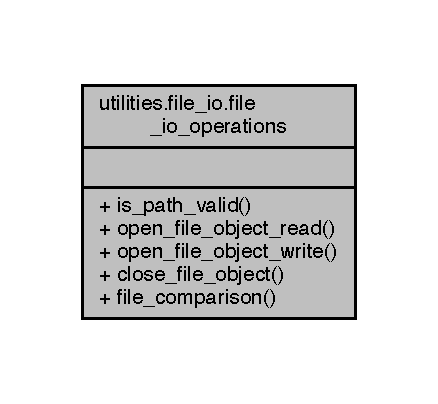
\includegraphics[width=210pt]{db/d83/classutilities_1_1file__io_1_1file__io__operations__coll__graph}
\end{center}
\end{figure}
\subsection*{Static Public Member Functions}
\begin{DoxyCompactItemize}
\item 
def \hyperlink{classutilities_1_1file__io_1_1file__io__operations_a1a7ef324955033ad370338fe37e68194}{open\+\_\+file\+\_\+object\+\_\+read} (filename)
\begin{DoxyCompactList}\small\item\em Method to open a file object for read/input operations. \end{DoxyCompactList}\item 
def \hyperlink{classutilities_1_1file__io_1_1file__io__operations_aaf94e26da1d988ece479d1600ad1de4a}{open\+\_\+file\+\_\+object\+\_\+write} (filename)
\begin{DoxyCompactList}\small\item\em Method to open a file object for write/output operations. \end{DoxyCompactList}\item 
def \hyperlink{classutilities_1_1file__io_1_1file__io__operations_a15cce5bd7767b057cdc569f393c24866}{close\+\_\+file\+\_\+object} (file\+\_\+obj)
\begin{DoxyCompactList}\small\item\em Method to close a file object. \end{DoxyCompactList}\item 
def \hyperlink{classutilities_1_1file__io_1_1file__io__operations_a9b3808ff6b165f5e73b780036f73a917}{file\+\_\+comparison} (file1, file2)
\begin{DoxyCompactList}\small\item\em Method to determine if two files are equivalent. \end{DoxyCompactList}\end{DoxyCompactItemize}


\subsection{Detailed Description}
Module with methods that perform file I/\+O operations. 



Definition at line \hyperlink{file__io_8py_source_l00051}{51} of file \hyperlink{file__io_8py_source}{file\+\_\+io.\+py}.



\subsection{Member Function Documentation}
\hypertarget{classutilities_1_1file__io_1_1file__io__operations_a15cce5bd7767b057cdc569f393c24866}{}\index{utilities\+::file\+\_\+io\+::file\+\_\+io\+\_\+operations@{utilities\+::file\+\_\+io\+::file\+\_\+io\+\_\+operations}!close\+\_\+file\+\_\+object@{close\+\_\+file\+\_\+object}}
\index{close\+\_\+file\+\_\+object@{close\+\_\+file\+\_\+object}!utilities\+::file\+\_\+io\+::file\+\_\+io\+\_\+operations@{utilities\+::file\+\_\+io\+::file\+\_\+io\+\_\+operations}}
\subsubsection[{close\+\_\+file\+\_\+object(file\+\_\+obj)}]{\setlength{\rightskip}{0pt plus 5cm}def utilities.\+file\+\_\+io.\+file\+\_\+io\+\_\+operations.\+close\+\_\+file\+\_\+object (
\begin{DoxyParamCaption}
\item[{}]{file\+\_\+obj}
\end{DoxyParamCaption}
)\hspace{0.3cm}{\ttfamily [static]}}\label{classutilities_1_1file__io_1_1file__io__operations_a15cce5bd7767b057cdc569f393c24866}


Method to close a file object. 

O(1) method. 

Definition at line \hyperlink{file__io_8py_source_l00070}{70} of file \hyperlink{file__io_8py_source}{file\+\_\+io.\+py}.


\begin{DoxyCode}
\hypertarget{classutilities_1_1file__io_1_1file__io__operations_l00070}{}\hyperlink{classutilities_1_1file__io_1_1file__io__operations_a15cce5bd7767b057cdc569f393c24866}{00070}     \textcolor{keyword}{def }\hyperlink{classutilities_1_1file__io_1_1file__io__operations_a15cce5bd7767b057cdc569f393c24866}{close\_file\_object}(file\_obj):
00071         file\_obj.close()
\end{DoxyCode}
\hypertarget{classutilities_1_1file__io_1_1file__io__operations_a9b3808ff6b165f5e73b780036f73a917}{}\index{utilities\+::file\+\_\+io\+::file\+\_\+io\+\_\+operations@{utilities\+::file\+\_\+io\+::file\+\_\+io\+\_\+operations}!file\+\_\+comparison@{file\+\_\+comparison}}
\index{file\+\_\+comparison@{file\+\_\+comparison}!utilities\+::file\+\_\+io\+::file\+\_\+io\+\_\+operations@{utilities\+::file\+\_\+io\+::file\+\_\+io\+\_\+operations}}
\subsubsection[{file\+\_\+comparison(file1, file2)}]{\setlength{\rightskip}{0pt plus 5cm}def utilities.\+file\+\_\+io.\+file\+\_\+io\+\_\+operations.\+file\+\_\+comparison (
\begin{DoxyParamCaption}
\item[{}]{file1, }
\item[{}]{file2}
\end{DoxyParamCaption}
)\hspace{0.3cm}{\ttfamily [static]}}\label{classutilities_1_1file__io_1_1file__io__operations_a9b3808ff6b165f5e73b780036f73a917}


Method to determine if two files are equivalent. 


\begin{DoxyParams}{Parameters}
{\em file1} & -\/ Path to a file. \\
\hline
{\em file2} & -\/ Path to another file. \\
\hline
\end{DoxyParams}
\begin{DoxyReturn}{Returns}
a boolean T\+R\+U\+E, if the files are equivalent. Else, return F\+A\+L\+S\+E. O(n) method, with respect to the number of lines in the larger (if the files are different), or either, of the files. 
\end{DoxyReturn}


Definition at line \hyperlink{file__io_8py_source_l00082}{82} of file \hyperlink{file__io_8py_source}{file\+\_\+io.\+py}.


\begin{DoxyCode}
\hypertarget{classutilities_1_1file__io_1_1file__io__operations_l00082}{}\hyperlink{classutilities_1_1file__io_1_1file__io__operations_a9b3808ff6b165f5e73b780036f73a917}{00082}     \textcolor{keyword}{def }\hyperlink{classutilities_1_1file__io_1_1file__io__operations_a9b3808ff6b165f5e73b780036f73a917}{file\_comparison}(file1, file2):
00083         \textcolor{keywordflow}{return} filecmp.cmp(file1,file2,shallow=\textcolor{keyword}{False})
00084 \end{DoxyCode}
\hypertarget{classutilities_1_1file__io_1_1file__io__operations_a1a7ef324955033ad370338fe37e68194}{}\index{utilities\+::file\+\_\+io\+::file\+\_\+io\+\_\+operations@{utilities\+::file\+\_\+io\+::file\+\_\+io\+\_\+operations}!open\+\_\+file\+\_\+object\+\_\+read@{open\+\_\+file\+\_\+object\+\_\+read}}
\index{open\+\_\+file\+\_\+object\+\_\+read@{open\+\_\+file\+\_\+object\+\_\+read}!utilities\+::file\+\_\+io\+::file\+\_\+io\+\_\+operations@{utilities\+::file\+\_\+io\+::file\+\_\+io\+\_\+operations}}
\subsubsection[{open\+\_\+file\+\_\+object\+\_\+read(filename)}]{\setlength{\rightskip}{0pt plus 5cm}def utilities.\+file\+\_\+io.\+file\+\_\+io\+\_\+operations.\+open\+\_\+file\+\_\+object\+\_\+read (
\begin{DoxyParamCaption}
\item[{}]{filename}
\end{DoxyParamCaption}
)\hspace{0.3cm}{\ttfamily [static]}}\label{classutilities_1_1file__io_1_1file__io__operations_a1a7ef324955033ad370338fe37e68194}


Method to open a file object for read/input operations. 

O(1) method. 

Definition at line \hyperlink{file__io_8py_source_l00056}{56} of file \hyperlink{file__io_8py_source}{file\+\_\+io.\+py}.


\begin{DoxyCode}
\hypertarget{classutilities_1_1file__io_1_1file__io__operations_l00056}{}\hyperlink{classutilities_1_1file__io_1_1file__io__operations_a1a7ef324955033ad370338fe37e68194}{00056}     \textcolor{keyword}{def }\hyperlink{classutilities_1_1file__io_1_1file__io__operations_a1a7ef324955033ad370338fe37e68194}{open\_file\_object\_read}(filename):
00057         ip\_file\_obj = open(filename, \textcolor{stringliteral}{'}\textcolor{stringliteral}{r')}
00058 \textcolor{stringliteral}{        }\textcolor{keywordflow}{return} ip\_file\_obj
\end{DoxyCode}
\hypertarget{classutilities_1_1file__io_1_1file__io__operations_aaf94e26da1d988ece479d1600ad1de4a}{}\index{utilities\+::file\+\_\+io\+::file\+\_\+io\+\_\+operations@{utilities\+::file\+\_\+io\+::file\+\_\+io\+\_\+operations}!open\+\_\+file\+\_\+object\+\_\+write@{open\+\_\+file\+\_\+object\+\_\+write}}
\index{open\+\_\+file\+\_\+object\+\_\+write@{open\+\_\+file\+\_\+object\+\_\+write}!utilities\+::file\+\_\+io\+::file\+\_\+io\+\_\+operations@{utilities\+::file\+\_\+io\+::file\+\_\+io\+\_\+operations}}
\subsubsection[{open\+\_\+file\+\_\+object\+\_\+write(filename)}]{\setlength{\rightskip}{0pt plus 5cm}def utilities.\+file\+\_\+io.\+file\+\_\+io\+\_\+operations.\+open\+\_\+file\+\_\+object\+\_\+write (
\begin{DoxyParamCaption}
\item[{}]{filename}
\end{DoxyParamCaption}
)\hspace{0.3cm}{\ttfamily [static]}}\label{classutilities_1_1file__io_1_1file__io__operations_aaf94e26da1d988ece479d1600ad1de4a}


Method to open a file object for write/output operations. 

O(1) method. 

Definition at line \hyperlink{file__io_8py_source_l00063}{63} of file \hyperlink{file__io_8py_source}{file\+\_\+io.\+py}.


\begin{DoxyCode}
\hypertarget{classutilities_1_1file__io_1_1file__io__operations_l00063}{}\hyperlink{classutilities_1_1file__io_1_1file__io__operations_aaf94e26da1d988ece479d1600ad1de4a}{00063}     \textcolor{keyword}{def }\hyperlink{classutilities_1_1file__io_1_1file__io__operations_aaf94e26da1d988ece479d1600ad1de4a}{open\_file\_object\_write}(filename):
00064         op\_file\_obj = open(filename, \textcolor{stringliteral}{'w'})
00065         \textcolor{keywordflow}{return} op\_file\_obj
\end{DoxyCode}


The documentation for this class was generated from the following file\+:\begin{DoxyCompactItemize}
\item 
utilities/\hyperlink{file__io_8py}{file\+\_\+io.\+py}\end{DoxyCompactItemize}

\hypertarget{classincremental__test_1_1Incremental__Test__Automation}{}\section{incremental\+\_\+test.\+Incremental\+\_\+\+Test\+\_\+\+Automation Class Reference}
\label{classincremental__test_1_1Incremental__Test__Automation}\index{incremental\+\_\+test.\+Incremental\+\_\+\+Test\+\_\+\+Automation@{incremental\+\_\+test.\+Incremental\+\_\+\+Test\+\_\+\+Automation}}


Collaboration diagram for incremental\+\_\+test.\+Incremental\+\_\+\+Test\+\_\+\+Automation\+:\nopagebreak
\begin{figure}[H]
\begin{center}
\leavevmode
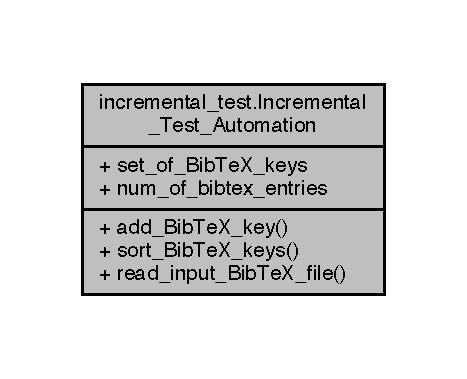
\includegraphics[width=224pt]{d3/d8e/classincremental__test_1_1Incremental__Test__Automation__coll__graph}
\end{center}
\end{figure}
\subsection*{Static Public Member Functions}
\begin{DoxyCompactItemize}
\item 
def \hyperlink{classincremental__test_1_1Incremental__Test__Automation_a14b316790ae1ef50d84bd4741a4fa020}{add\+\_\+\+Bib\+Te\+X\+\_\+key} (found\+\_\+\+Bib\+Te\+X\+\_\+key)
\begin{DoxyCompactList}\small\item\em Method to add Bib\+Te\+X keys into a list, \char`\"{}set\+\_\+of\+\_\+\+Bib\+Te\+X\+\_\+keys\char`\"{}. \end{DoxyCompactList}\item 
def \hyperlink{classincremental__test_1_1Incremental__Test__Automation_a856c60714b5d716d5eb630cbc3d55d09}{sort\+\_\+\+Bib\+Te\+X\+\_\+keys} ()
\begin{DoxyCompactList}\small\item\em Method to sort Bib\+Te\+X keys into a list, \char`\"{}set\+\_\+of\+\_\+\+Bib\+Te\+X\+\_\+keys\char`\"{}. \end{DoxyCompactList}\item 
def \hyperlink{classincremental__test_1_1Incremental__Test__Automation_a7cec6a541c4680c857a699dbe363ffbd}{read\+\_\+input\+\_\+\+Bib\+Te\+X\+\_\+file} (ip\+\_\+file\+\_\+object, input\+\_\+\+Bib\+Te\+X\+\_\+file)
\begin{DoxyCompactList}\small\item\em Method to read each line of the input Bib\+Te\+X file. \end{DoxyCompactList}\end{DoxyCompactItemize}
\subsection*{Static Public Attributes}
\begin{DoxyCompactItemize}
\item 
list \hyperlink{classincremental__test_1_1Incremental__Test__Automation_a8f5272e0488026aa24a829262392f2f7}{set\+\_\+of\+\_\+\+Bib\+Te\+X\+\_\+keys} = \mbox{[}$\,$\mbox{]}
\item 
int \hyperlink{classincremental__test_1_1Incremental__Test__Automation_ac60587acca9d28d055bd8a7198a987a1}{num\+\_\+of\+\_\+bibtex\+\_\+entries} = 0
\end{DoxyCompactItemize}


\subsection{Detailed Description}


Definition at line \hyperlink{incremental__test_8py_source_l00110}{110} of file \hyperlink{incremental__test_8py_source}{incremental\+\_\+test.\+py}.



\subsection{Member Function Documentation}
\hypertarget{classincremental__test_1_1Incremental__Test__Automation_a14b316790ae1ef50d84bd4741a4fa020}{}\index{incremental\+\_\+test\+::\+Incremental\+\_\+\+Test\+\_\+\+Automation@{incremental\+\_\+test\+::\+Incremental\+\_\+\+Test\+\_\+\+Automation}!add\+\_\+\+Bib\+Te\+X\+\_\+key@{add\+\_\+\+Bib\+Te\+X\+\_\+key}}
\index{add\+\_\+\+Bib\+Te\+X\+\_\+key@{add\+\_\+\+Bib\+Te\+X\+\_\+key}!incremental\+\_\+test\+::\+Incremental\+\_\+\+Test\+\_\+\+Automation@{incremental\+\_\+test\+::\+Incremental\+\_\+\+Test\+\_\+\+Automation}}
\subsubsection[{add\+\_\+\+Bib\+Te\+X\+\_\+key(found\+\_\+\+Bib\+Te\+X\+\_\+key)}]{\setlength{\rightskip}{0pt plus 5cm}def incremental\+\_\+test.\+Incremental\+\_\+\+Test\+\_\+\+Automation.\+add\+\_\+\+Bib\+Te\+X\+\_\+key (
\begin{DoxyParamCaption}
\item[{}]{found\+\_\+\+Bib\+Te\+X\+\_\+key}
\end{DoxyParamCaption}
)\hspace{0.3cm}{\ttfamily [static]}}\label{classincremental__test_1_1Incremental__Test__Automation_a14b316790ae1ef50d84bd4741a4fa020}


Method to add Bib\+Te\+X keys into a list, \char`\"{}set\+\_\+of\+\_\+\+Bib\+Te\+X\+\_\+keys\char`\"{}. 

O(n) method, where n is the number of Bib\+Te\+X keys. 

Definition at line \hyperlink{incremental__test_8py_source_l00120}{120} of file \hyperlink{incremental__test_8py_source}{incremental\+\_\+test.\+py}.


\begin{DoxyCode}
\hypertarget{classincremental__test_1_1Incremental__Test__Automation_l00120}{}\hyperlink{classincremental__test_1_1Incremental__Test__Automation_a14b316790ae1ef50d84bd4741a4fa020}{00120}     \textcolor{keyword}{def }\hyperlink{classincremental__test_1_1Incremental__Test__Automation_a14b316790ae1ef50d84bd4741a4fa020}{add\_BibTeX\_key}(found\_BibTeX\_key):
00121         \textcolor{keywordflow}{if} (found\_BibTeX\_key \textcolor{keywordflow}{in} Incremental\_Test\_Automation.set\_of\_BibTeX\_keys):
00122             temp\_str = \textcolor{stringliteral}{"Duplicate BibTeX key:"}+found\_BibTeX\_key
00123             warnings.warn(temp\_str)
00124             \textcolor{keywordflow}{raise} Exception(\textcolor{stringliteral}{"Multiple instances of a BibTeX key"})
00125         Incremental\_Test\_Automation.set\_of\_BibTeX\_keys.append(found\_BibTeX\_key)
\end{DoxyCode}
\hypertarget{classincremental__test_1_1Incremental__Test__Automation_a7cec6a541c4680c857a699dbe363ffbd}{}\index{incremental\+\_\+test\+::\+Incremental\+\_\+\+Test\+\_\+\+Automation@{incremental\+\_\+test\+::\+Incremental\+\_\+\+Test\+\_\+\+Automation}!read\+\_\+input\+\_\+\+Bib\+Te\+X\+\_\+file@{read\+\_\+input\+\_\+\+Bib\+Te\+X\+\_\+file}}
\index{read\+\_\+input\+\_\+\+Bib\+Te\+X\+\_\+file@{read\+\_\+input\+\_\+\+Bib\+Te\+X\+\_\+file}!incremental\+\_\+test\+::\+Incremental\+\_\+\+Test\+\_\+\+Automation@{incremental\+\_\+test\+::\+Incremental\+\_\+\+Test\+\_\+\+Automation}}
\subsubsection[{read\+\_\+input\+\_\+\+Bib\+Te\+X\+\_\+file(ip\+\_\+file\+\_\+object, input\+\_\+\+Bib\+Te\+X\+\_\+file)}]{\setlength{\rightskip}{0pt plus 5cm}def incremental\+\_\+test.\+Incremental\+\_\+\+Test\+\_\+\+Automation.\+read\+\_\+input\+\_\+\+Bib\+Te\+X\+\_\+file (
\begin{DoxyParamCaption}
\item[{}]{ip\+\_\+file\+\_\+object, }
\item[{}]{input\+\_\+\+Bib\+Te\+X\+\_\+file}
\end{DoxyParamCaption}
)\hspace{0.3cm}{\ttfamily [static]}}\label{classincremental__test_1_1Incremental__Test__Automation_a7cec6a541c4680c857a699dbe363ffbd}


Method to read each line of the input Bib\+Te\+X file. 

O(n) method, where n is the number of lines of the Bib\+Te\+X file. 

Definition at line \hyperlink{incremental__test_8py_source_l00136}{136} of file \hyperlink{incremental__test_8py_source}{incremental\+\_\+test.\+py}.


\begin{DoxyCode}
\hypertarget{classincremental__test_1_1Incremental__Test__Automation_l00136}{}\hyperlink{classincremental__test_1_1Incremental__Test__Automation_a7cec6a541c4680c857a699dbe363ffbd}{00136}     \textcolor{keyword}{def }\hyperlink{classincremental__test_1_1Incremental__Test__Automation_a7cec6a541c4680c857a699dbe363ffbd}{read\_input\_BibTeX\_file}(ip\_file\_object,input\_BibTeX\_file):
00137         \textcolor{comment}{#print "--------------------------------------------------------"}
00138         println = \textcolor{stringliteral}{"=    Reading input BibTeX file: "}
00139         println += input\_BibTeX\_file
00140         print(println)
00141         \textcolor{comment}{# Read each available line in the input BibTeX file.}
00142         \textcolor{keywordflow}{for} line \textcolor{keywordflow}{in} ip\_file\_object:
00143             \textcolor{comment}{# Is this line the 1st line of a BibTeX entry?}
00144             \textcolor{keywordflow}{if} \textcolor{stringliteral}{"@"} == line[0]:
00145                 \textcolor{comment}{# Yes.}
00146 \textcolor{comment}{#               print "...  First line of a BibTeX entry."}
00147                 \textcolor{comment}{# Increment number of BibTeX entries.}
00148                 Incremental\_Test\_Automation.num\_of\_bibtex\_entries = 
      Incremental\_Test\_Automation.num\_of\_bibtex\_entries + 1
00149                 tokenized\_BibTeX\_entry = re.split(\textcolor{stringliteral}{'@|\{|,'},line)
00150 \textcolor{comment}{#               for i in tokenized\_BibTeX\_entry:}
00151 \textcolor{comment}{#                   print i}
00152                 \textcolor{comment}{# Is the type of the BibTeX entry valid?}
00153                 \textcolor{keywordflow}{if} (tokenized\_BibTeX\_entry[1] \textcolor{keywordflow}{in} queue\_ip\_args.BibTeX\_entry\_types):
00154                     \textcolor{comment}{# Yes. Try adding the BibTeX entry to "set\_of\_BibTeX\_keys".}
00155                     Incremental\_Test\_Automation.add\_BibTeX\_key(tokenized\_BibTeX\_entry[2].lower())
00156                 \textcolor{keywordflow}{else}:
00157                     \textcolor{comment}{# No. Warn user that the type of BibTeX entry is invalid!}
00158                     temp\_str = \textcolor{stringliteral}{"Invalid type of BibTeX entry:"}
00159                     temp\_str += tokenized\_BibTeX\_entry[1]
00160                     print(temp\_str)
00161                     \textcolor{comment}{#warnings.warn("Invalid type of BibTeX entry")}
00162                     \textcolor{keywordflow}{raise} Exception(\textcolor{stringliteral}{"BibTeX entry has an invalid type!"})
00163         \textcolor{keywordflow}{if} (Incremental\_Test\_Automation.num\_of\_bibtex\_entries != len(
      Incremental\_Test\_Automation.set\_of\_BibTeX\_keys)):
00164             \textcolor{keywordflow}{raise} Exception(\textcolor{stringliteral}{"Mismatch in number of BibTeX entries processed."})
00165         \textcolor{keywordflow}{else}:
00166             print(\textcolor{stringliteral}{"=    Number of BibTeX entries processed: \{\}"} .format(str(
      Incremental\_Test\_Automation.num\_of\_bibtex\_entries)))
00167 
00168 
00169 
00170 
00171 
00172 
00173 
00174 
00175 
00176 
00177 
\end{DoxyCode}
\hypertarget{classincremental__test_1_1Incremental__Test__Automation_a856c60714b5d716d5eb630cbc3d55d09}{}\index{incremental\+\_\+test\+::\+Incremental\+\_\+\+Test\+\_\+\+Automation@{incremental\+\_\+test\+::\+Incremental\+\_\+\+Test\+\_\+\+Automation}!sort\+\_\+\+Bib\+Te\+X\+\_\+keys@{sort\+\_\+\+Bib\+Te\+X\+\_\+keys}}
\index{sort\+\_\+\+Bib\+Te\+X\+\_\+keys@{sort\+\_\+\+Bib\+Te\+X\+\_\+keys}!incremental\+\_\+test\+::\+Incremental\+\_\+\+Test\+\_\+\+Automation@{incremental\+\_\+test\+::\+Incremental\+\_\+\+Test\+\_\+\+Automation}}
\subsubsection[{sort\+\_\+\+Bib\+Te\+X\+\_\+keys()}]{\setlength{\rightskip}{0pt plus 5cm}def incremental\+\_\+test.\+Incremental\+\_\+\+Test\+\_\+\+Automation.\+sort\+\_\+\+Bib\+Te\+X\+\_\+keys (
\begin{DoxyParamCaption}
{}
\end{DoxyParamCaption}
)\hspace{0.3cm}{\ttfamily [static]}}\label{classincremental__test_1_1Incremental__Test__Automation_a856c60714b5d716d5eb630cbc3d55d09}


Method to sort Bib\+Te\+X keys into a list, \char`\"{}set\+\_\+of\+\_\+\+Bib\+Te\+X\+\_\+keys\char`\"{}. 

O(n$\ast$log(n)) method, where n is the number of Bib\+Te\+X keys. 

Definition at line \hyperlink{incremental__test_8py_source_l00130}{130} of file \hyperlink{incremental__test_8py_source}{incremental\+\_\+test.\+py}.


\begin{DoxyCode}
\hypertarget{classincremental__test_1_1Incremental__Test__Automation_l00130}{}\hyperlink{classincremental__test_1_1Incremental__Test__Automation_a856c60714b5d716d5eb630cbc3d55d09}{00130}     \textcolor{keyword}{def }\hyperlink{classincremental__test_1_1Incremental__Test__Automation_a856c60714b5d716d5eb630cbc3d55d09}{sort\_BibTeX\_keys}():
00131         Incremental\_Test\_Automation.set\_of\_BibTeX\_keys = sorted(
      Incremental\_Test\_Automation.set\_of\_BibTeX\_keys)
\end{DoxyCode}


\subsection{Member Data Documentation}
\hypertarget{classincremental__test_1_1Incremental__Test__Automation_ac60587acca9d28d055bd8a7198a987a1}{}\index{incremental\+\_\+test\+::\+Incremental\+\_\+\+Test\+\_\+\+Automation@{incremental\+\_\+test\+::\+Incremental\+\_\+\+Test\+\_\+\+Automation}!num\+\_\+of\+\_\+bibtex\+\_\+entries@{num\+\_\+of\+\_\+bibtex\+\_\+entries}}
\index{num\+\_\+of\+\_\+bibtex\+\_\+entries@{num\+\_\+of\+\_\+bibtex\+\_\+entries}!incremental\+\_\+test\+::\+Incremental\+\_\+\+Test\+\_\+\+Automation@{incremental\+\_\+test\+::\+Incremental\+\_\+\+Test\+\_\+\+Automation}}
\subsubsection[{num\+\_\+of\+\_\+bibtex\+\_\+entries}]{\setlength{\rightskip}{0pt plus 5cm}int incremental\+\_\+test.\+Incremental\+\_\+\+Test\+\_\+\+Automation.\+num\+\_\+of\+\_\+bibtex\+\_\+entries = 0\hspace{0.3cm}{\ttfamily [static]}}\label{classincremental__test_1_1Incremental__Test__Automation_ac60587acca9d28d055bd8a7198a987a1}


Definition at line \hyperlink{incremental__test_8py_source_l00113}{113} of file \hyperlink{incremental__test_8py_source}{incremental\+\_\+test.\+py}.

\hypertarget{classincremental__test_1_1Incremental__Test__Automation_a8f5272e0488026aa24a829262392f2f7}{}\index{incremental\+\_\+test\+::\+Incremental\+\_\+\+Test\+\_\+\+Automation@{incremental\+\_\+test\+::\+Incremental\+\_\+\+Test\+\_\+\+Automation}!set\+\_\+of\+\_\+\+Bib\+Te\+X\+\_\+keys@{set\+\_\+of\+\_\+\+Bib\+Te\+X\+\_\+keys}}
\index{set\+\_\+of\+\_\+\+Bib\+Te\+X\+\_\+keys@{set\+\_\+of\+\_\+\+Bib\+Te\+X\+\_\+keys}!incremental\+\_\+test\+::\+Incremental\+\_\+\+Test\+\_\+\+Automation@{incremental\+\_\+test\+::\+Incremental\+\_\+\+Test\+\_\+\+Automation}}
\subsubsection[{set\+\_\+of\+\_\+\+Bib\+Te\+X\+\_\+keys}]{\setlength{\rightskip}{0pt plus 5cm}list incremental\+\_\+test.\+Incremental\+\_\+\+Test\+\_\+\+Automation.\+set\+\_\+of\+\_\+\+Bib\+Te\+X\+\_\+keys = \mbox{[}$\,$\mbox{]}\hspace{0.3cm}{\ttfamily [static]}}\label{classincremental__test_1_1Incremental__Test__Automation_a8f5272e0488026aa24a829262392f2f7}


Definition at line \hyperlink{incremental__test_8py_source_l00112}{112} of file \hyperlink{incremental__test_8py_source}{incremental\+\_\+test.\+py}.



The documentation for this class was generated from the following file\+:\begin{DoxyCompactItemize}
\item 
\hyperlink{incremental__test_8py}{incremental\+\_\+test.\+py}\end{DoxyCompactItemize}

\hypertarget{classutilities_1_1queue__ip__arguments_1_1queue__ip__args}{}\section{utilities.\+queue\+\_\+ip\+\_\+arguments.\+queue\+\_\+ip\+\_\+args Class Reference}
\label{classutilities_1_1queue__ip__arguments_1_1queue__ip__args}\index{utilities.\+queue\+\_\+ip\+\_\+arguments.\+queue\+\_\+ip\+\_\+args@{utilities.\+queue\+\_\+ip\+\_\+arguments.\+queue\+\_\+ip\+\_\+args}}


Import Custom Python Modules.  




Collaboration diagram for utilities.\+queue\+\_\+ip\+\_\+arguments.\+queue\+\_\+ip\+\_\+args\+:\nopagebreak
\begin{figure}[H]
\begin{center}
\leavevmode
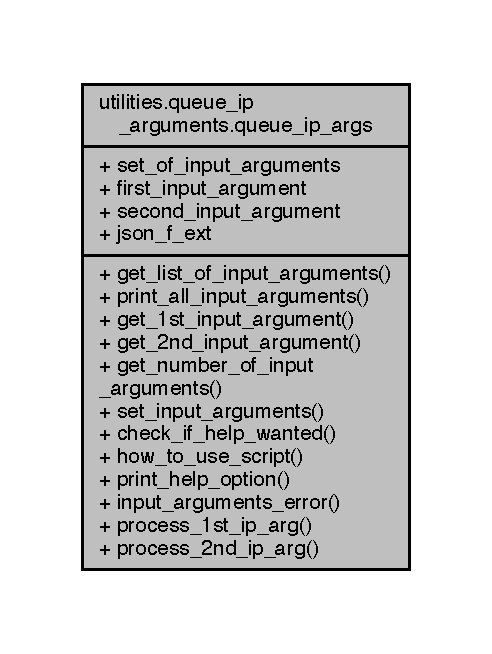
\includegraphics[width=226pt]{d0/dae/classutilities_1_1queue__ip__arguments_1_1queue__ip__args__coll__graph}
\end{center}
\end{figure}
\subsection*{Static Public Member Functions}
\begin{DoxyCompactItemize}
\item 
def \hyperlink{classutilities_1_1queue__ip__arguments_1_1queue__ip__args_abeea0f35fe270bfe53f359fd8e85c3e0}{get\+\_\+input\+\_\+arguments} ()
\begin{DoxyCompactList}\small\item\em Method to get the input arguments. \end{DoxyCompactList}\item 
def \hyperlink{classutilities_1_1queue__ip__arguments_1_1queue__ip__args_a85480b443e2538123e8531852f9035c9}{print\+\_\+all\+\_\+input\+\_\+arguments} ()
\begin{DoxyCompactList}\small\item\em Method to print all the input arguments. \end{DoxyCompactList}\item 
def \hyperlink{classutilities_1_1queue__ip__arguments_1_1queue__ip__args_a7b3c5efad539fadfb53eda0cfb8d3f03}{get\+\_\+1st\+\_\+input\+\_\+argument} ()
\begin{DoxyCompactList}\small\item\em Method to get the first input argument. \end{DoxyCompactList}\item 
def \hyperlink{classutilities_1_1queue__ip__arguments_1_1queue__ip__args_a18e59da1e2c8044e79ca32a5455ef40b}{get\+\_\+2nd\+\_\+input\+\_\+argument} ()
\begin{DoxyCompactList}\small\item\em Method to get the second input argument. \end{DoxyCompactList}\item 
def \hyperlink{classutilities_1_1queue__ip__arguments_1_1queue__ip__args_ab95a4242fd55bf5d126b35a5f5172593}{get\+\_\+number\+\_\+of\+\_\+input\+\_\+arguments} ()
\begin{DoxyCompactList}\small\item\em Method to get the number of input arguments. \end{DoxyCompactList}\item 
def \hyperlink{classutilities_1_1queue__ip__arguments_1_1queue__ip__args_a9eb36bdd493a2c866460b4d9fb24b68c}{get\+\_\+name\+\_\+of\+\_\+current\+\_\+script} ()
\begin{DoxyCompactList}\small\item\em Method to get the name of the current script that is being executed. \end{DoxyCompactList}\item 
def \hyperlink{classutilities_1_1queue__ip__arguments_1_1queue__ip__args_a4c536970af155ee6cc2c2886b145f807}{set\+\_\+input\+\_\+arguments} (list\+\_\+of\+\_\+ip\+\_\+arguments, which\+\_\+script)
\begin{DoxyCompactList}\small\item\em Method to set the input arguments. \end{DoxyCompactList}\item 
def \hyperlink{classutilities_1_1queue__ip__arguments_1_1queue__ip__args_a1a87ae4035acfa51fe1d1aff53f770f3}{check\+\_\+if\+\_\+help\+\_\+wanted} ()
\begin{DoxyCompactList}\small\item\em Method to determine if the user wants help, and conequently display the user manual. \end{DoxyCompactList}\item 
def \hyperlink{classutilities_1_1queue__ip__arguments_1_1queue__ip__args_a5fecd33a91d20f19acba2fb1b8d1a60e}{how\+\_\+to\+\_\+use\+\_\+script} ()
\begin{DoxyCompactList}\small\item\em Method to provide information on how to run this script. \end{DoxyCompactList}\item 
def \hyperlink{classutilities_1_1queue__ip__arguments_1_1queue__ip__args_a6311efe4f2f6ac8c64c9b442e8854ab7}{print\+\_\+2nd\+\_\+argument} ()
\begin{DoxyCompactList}\small\item\em Method to provide information on the second input argument. \end{DoxyCompactList}\item 
def \hyperlink{classutilities_1_1queue__ip__arguments_1_1queue__ip__args_a28c79307da87e28e9ac3467290fd5738}{print\+\_\+help\+\_\+option} ()
\begin{DoxyCompactList}\small\item\em Method to print the help option to access the user manual. \end{DoxyCompactList}\item 
def \hyperlink{classutilities_1_1queue__ip__arguments_1_1queue__ip__args_afdfbfffba8afb5e786283dd22d856e93}{input\+\_\+arguments\+\_\+error} ()
\begin{DoxyCompactList}\small\item\em Method to indicate error wth input arguments. \end{DoxyCompactList}\item 
def \hyperlink{classutilities_1_1queue__ip__arguments_1_1queue__ip__args_ae1fc6d7af2e429d0656dbf388711db94}{process\+\_\+1st\+\_\+ip\+\_\+arg} ()
\begin{DoxyCompactList}\small\item\em Method to process the first input argument. \end{DoxyCompactList}\item 
def \hyperlink{classutilities_1_1queue__ip__arguments_1_1queue__ip__args_a82d245379c48196f61d4268882dd5c6d}{process\+\_\+2nd\+\_\+ip\+\_\+arg} ()
\begin{DoxyCompactList}\small\item\em Method to process the second input argument. \end{DoxyCompactList}\item 
def \hyperlink{classutilities_1_1queue__ip__arguments_1_1queue__ip__args_a4420d4d6a1272816131b5426bfaf678e}{missing\+\_\+2nd\+\_\+ip\+\_\+arg} ()
\begin{DoxyCompactList}\small\item\em Method to handle missing second input argument. \end{DoxyCompactList}\end{DoxyCompactItemize}
\subsection*{Static Public Attributes}
\begin{DoxyCompactItemize}
\item 
list \hyperlink{classutilities_1_1queue__ip__arguments_1_1queue__ip__args_acc8e7685be71a7f95ede7c980355c9f3}{set\+\_\+of\+\_\+input\+\_\+arguments} = \mbox{[}$\,$\mbox{]}
\item 
string \hyperlink{classutilities_1_1queue__ip__arguments_1_1queue__ip__args_a14394c9820086e09d5b926d9910a180f}{first\+\_\+input\+\_\+argument} = \char`\"{}First input argument.\char`\"{}
\item 
string \hyperlink{classutilities_1_1queue__ip__arguments_1_1queue__ip__args_a0b179a70c0e57de2794d0d532e534c9c}{second\+\_\+input\+\_\+argument} = \char`\"{}Second input argument.\char`\"{}
\item 
string \hyperlink{classutilities_1_1queue__ip__arguments_1_1queue__ip__args_a8d93f9ade7608583602a9948c0d744f7}{json\+\_\+f\+\_\+ext} = \char`\"{}.json\char`\"{}
\item 
string \hyperlink{classutilities_1_1queue__ip__arguments_1_1queue__ip__args_a453711109bd635e6263a99c8e85e3dff}{C\+U\+R\+R\+E\+N\+T\+\_\+\+S\+C\+R\+I\+P\+T} = \char`\"{}No script is currently being executed.\char`\"{}
\item 
string \hyperlink{classutilities_1_1queue__ip__arguments_1_1queue__ip__args_a849b659d7a9d7689c4c707502d1684d5}{I\+N\+C\+R\+E\+M\+E\+N\+T\+A\+L\+\_\+\+T\+E\+S\+T} = \char`\"{}incremental\+\_\+test.\+py\char`\"{}
\item 
string \hyperlink{classutilities_1_1queue__ip__arguments_1_1queue__ip__args_ad61d6e7f7e2602c0f1c11a8fdf2b7168}{P\+R\+O\+B\+L\+E\+M1\+\_\+\+S\+O\+L\+U\+T\+I\+O\+N} = \char`\"{}problem1\+\_\+solution.\+py\char`\"{}
\end{DoxyCompactItemize}


\subsection{Detailed Description}
Import Custom Python Modules. 

Module with methods that clean Bib\+Te\+X files. 

Definition at line \hyperlink{queue__ip__arguments_8py_source_l00073}{73} of file \hyperlink{queue__ip__arguments_8py_source}{queue\+\_\+ip\+\_\+arguments.\+py}.



\subsection{Member Function Documentation}
\hypertarget{classutilities_1_1queue__ip__arguments_1_1queue__ip__args_a1a87ae4035acfa51fe1d1aff53f770f3}{}\index{utilities\+::queue\+\_\+ip\+\_\+arguments\+::queue\+\_\+ip\+\_\+args@{utilities\+::queue\+\_\+ip\+\_\+arguments\+::queue\+\_\+ip\+\_\+args}!check\+\_\+if\+\_\+help\+\_\+wanted@{check\+\_\+if\+\_\+help\+\_\+wanted}}
\index{check\+\_\+if\+\_\+help\+\_\+wanted@{check\+\_\+if\+\_\+help\+\_\+wanted}!utilities\+::queue\+\_\+ip\+\_\+arguments\+::queue\+\_\+ip\+\_\+args@{utilities\+::queue\+\_\+ip\+\_\+arguments\+::queue\+\_\+ip\+\_\+args}}
\subsubsection[{check\+\_\+if\+\_\+help\+\_\+wanted()}]{\setlength{\rightskip}{0pt plus 5cm}def utilities.\+queue\+\_\+ip\+\_\+arguments.\+queue\+\_\+ip\+\_\+args.\+check\+\_\+if\+\_\+help\+\_\+wanted (
\begin{DoxyParamCaption}
{}
\end{DoxyParamCaption}
)\hspace{0.3cm}{\ttfamily [static]}}\label{classutilities_1_1queue__ip__arguments_1_1queue__ip__args_a1a87ae4035acfa51fe1d1aff53f770f3}


Method to determine if the user wants help, and conequently display the user manual. 

O(n) method, with respect to the number of input arguments. 

Definition at line \hyperlink{queue__ip__arguments_8py_source_l00169}{169} of file \hyperlink{queue__ip__arguments_8py_source}{queue\+\_\+ip\+\_\+arguments.\+py}.


\begin{DoxyCode}
\hypertarget{classutilities_1_1queue__ip__arguments_1_1queue__ip__args_l00169}{}\hyperlink{classutilities_1_1queue__ip__arguments_1_1queue__ip__args_a1a87ae4035acfa51fe1d1aff53f770f3}{00169}     \textcolor{keyword}{def }\hyperlink{classutilities_1_1queue__ip__arguments_1_1queue__ip__args_a1a87ae4035acfa51fe1d1aff53f770f3}{check\_if\_help\_wanted}():
00170         \textcolor{comment}{# If user wants to read the brief user manual,}
00171         \textcolor{keywordflow}{if} \textcolor{stringliteral}{"-h"} \textcolor{keywordflow}{in} queue\_ip\_args.set\_of\_input\_arguments:
00172             \textcolor{comment}{# Display the user manual and exit.}
00173             queue\_ip\_args.how\_to\_use\_script()
00174             sys.exit()
\end{DoxyCode}
\hypertarget{classutilities_1_1queue__ip__arguments_1_1queue__ip__args_a7b3c5efad539fadfb53eda0cfb8d3f03}{}\index{utilities\+::queue\+\_\+ip\+\_\+arguments\+::queue\+\_\+ip\+\_\+args@{utilities\+::queue\+\_\+ip\+\_\+arguments\+::queue\+\_\+ip\+\_\+args}!get\+\_\+1st\+\_\+input\+\_\+argument@{get\+\_\+1st\+\_\+input\+\_\+argument}}
\index{get\+\_\+1st\+\_\+input\+\_\+argument@{get\+\_\+1st\+\_\+input\+\_\+argument}!utilities\+::queue\+\_\+ip\+\_\+arguments\+::queue\+\_\+ip\+\_\+args@{utilities\+::queue\+\_\+ip\+\_\+arguments\+::queue\+\_\+ip\+\_\+args}}
\subsubsection[{get\+\_\+1st\+\_\+input\+\_\+argument()}]{\setlength{\rightskip}{0pt plus 5cm}def utilities.\+queue\+\_\+ip\+\_\+arguments.\+queue\+\_\+ip\+\_\+args.\+get\+\_\+1st\+\_\+input\+\_\+argument (
\begin{DoxyParamCaption}
{}
\end{DoxyParamCaption}
)\hspace{0.3cm}{\ttfamily [static]}}\label{classutilities_1_1queue__ip__arguments_1_1queue__ip__args_a7b3c5efad539fadfb53eda0cfb8d3f03}


Method to get the first input argument. 

\begin{DoxyReturn}{Returns}
-\/ First input argument for the program. O(1) method. 
\end{DoxyReturn}


Definition at line \hyperlink{queue__ip__arguments_8py_source_l00114}{114} of file \hyperlink{queue__ip__arguments_8py_source}{queue\+\_\+ip\+\_\+arguments.\+py}.


\begin{DoxyCode}
\hypertarget{classutilities_1_1queue__ip__arguments_1_1queue__ip__args_l00114}{}\hyperlink{classutilities_1_1queue__ip__arguments_1_1queue__ip__args_a7b3c5efad539fadfb53eda0cfb8d3f03}{00114}     \textcolor{keyword}{def }\hyperlink{classutilities_1_1queue__ip__arguments_1_1queue__ip__args_a7b3c5efad539fadfb53eda0cfb8d3f03}{get\_1st\_input\_argument}():
00115         \textcolor{keywordflow}{if} 0 < len(queue\_ip\_args.get\_input\_arguments()):
00116             \textcolor{keywordflow}{return} queue\_ip\_args.set\_of\_input\_arguments[0]
00117         \textcolor{keywordflow}{else}:
00118             warnings.warn(\textcolor{stringliteral}{" 1st input argument is missing!!!"})
00119             queue\_ip\_args.input\_arguments\_error()
\end{DoxyCode}
\hypertarget{classutilities_1_1queue__ip__arguments_1_1queue__ip__args_a18e59da1e2c8044e79ca32a5455ef40b}{}\index{utilities\+::queue\+\_\+ip\+\_\+arguments\+::queue\+\_\+ip\+\_\+args@{utilities\+::queue\+\_\+ip\+\_\+arguments\+::queue\+\_\+ip\+\_\+args}!get\+\_\+2nd\+\_\+input\+\_\+argument@{get\+\_\+2nd\+\_\+input\+\_\+argument}}
\index{get\+\_\+2nd\+\_\+input\+\_\+argument@{get\+\_\+2nd\+\_\+input\+\_\+argument}!utilities\+::queue\+\_\+ip\+\_\+arguments\+::queue\+\_\+ip\+\_\+args@{utilities\+::queue\+\_\+ip\+\_\+arguments\+::queue\+\_\+ip\+\_\+args}}
\subsubsection[{get\+\_\+2nd\+\_\+input\+\_\+argument()}]{\setlength{\rightskip}{0pt plus 5cm}def utilities.\+queue\+\_\+ip\+\_\+arguments.\+queue\+\_\+ip\+\_\+args.\+get\+\_\+2nd\+\_\+input\+\_\+argument (
\begin{DoxyParamCaption}
{}
\end{DoxyParamCaption}
)\hspace{0.3cm}{\ttfamily [static]}}\label{classutilities_1_1queue__ip__arguments_1_1queue__ip__args_a18e59da1e2c8044e79ca32a5455ef40b}


Method to get the second input argument. 

\begin{DoxyReturn}{Returns}
-\/ Second input argument for the program. O(1) method. 
\end{DoxyReturn}


Definition at line \hyperlink{queue__ip__arguments_8py_source_l00125}{125} of file \hyperlink{queue__ip__arguments_8py_source}{queue\+\_\+ip\+\_\+arguments.\+py}.


\begin{DoxyCode}
\hypertarget{classutilities_1_1queue__ip__arguments_1_1queue__ip__args_l00125}{}\hyperlink{classutilities_1_1queue__ip__arguments_1_1queue__ip__args_a18e59da1e2c8044e79ca32a5455ef40b}{00125}     \textcolor{keyword}{def }\hyperlink{classutilities_1_1queue__ip__arguments_1_1queue__ip__args_a18e59da1e2c8044e79ca32a5455ef40b}{get\_2nd\_input\_argument}():
00126         \textcolor{keywordflow}{if} 1 < len(queue\_ip\_args.get\_input\_arguments()):
00127             \textcolor{keywordflow}{return} queue\_ip\_args.set\_of\_input\_arguments[1]
00128         \textcolor{keywordflow}{else}:
00129             warnings.warn(\textcolor{stringliteral}{" 2nd input argument is missing!!!"})
00130             queue\_ip\_args.input\_arguments\_error()
\end{DoxyCode}
\hypertarget{classutilities_1_1queue__ip__arguments_1_1queue__ip__args_abeea0f35fe270bfe53f359fd8e85c3e0}{}\index{utilities\+::queue\+\_\+ip\+\_\+arguments\+::queue\+\_\+ip\+\_\+args@{utilities\+::queue\+\_\+ip\+\_\+arguments\+::queue\+\_\+ip\+\_\+args}!get\+\_\+input\+\_\+arguments@{get\+\_\+input\+\_\+arguments}}
\index{get\+\_\+input\+\_\+arguments@{get\+\_\+input\+\_\+arguments}!utilities\+::queue\+\_\+ip\+\_\+arguments\+::queue\+\_\+ip\+\_\+args@{utilities\+::queue\+\_\+ip\+\_\+arguments\+::queue\+\_\+ip\+\_\+args}}
\subsubsection[{get\+\_\+input\+\_\+arguments()}]{\setlength{\rightskip}{0pt plus 5cm}def utilities.\+queue\+\_\+ip\+\_\+arguments.\+queue\+\_\+ip\+\_\+args.\+get\+\_\+input\+\_\+arguments (
\begin{DoxyParamCaption}
{}
\end{DoxyParamCaption}
)\hspace{0.3cm}{\ttfamily [static]}}\label{classutilities_1_1queue__ip__arguments_1_1queue__ip__args_abeea0f35fe270bfe53f359fd8e85c3e0}


Method to get the input arguments. 

\begin{DoxyReturn}{Returns}
-\/ List of input arguments to the program. O(1) method. \begin{DoxyVerb}print "=    Set_of_input_arguments:"
for cur_ip_arg in queue_ip_args.set_of_input_arguments:
    print " "+cur_ip_arg
\end{DoxyVerb}
 
\end{DoxyReturn}


Definition at line \hyperlink{queue__ip__arguments_8py_source_l00094}{94} of file \hyperlink{queue__ip__arguments_8py_source}{queue\+\_\+ip\+\_\+arguments.\+py}.


\begin{DoxyCode}
\hypertarget{classutilities_1_1queue__ip__arguments_1_1queue__ip__args_l00094}{}\hyperlink{classutilities_1_1queue__ip__arguments_1_1queue__ip__args_abeea0f35fe270bfe53f359fd8e85c3e0}{00094}     \textcolor{keyword}{def }\hyperlink{classutilities_1_1queue__ip__arguments_1_1queue__ip__args_abeea0f35fe270bfe53f359fd8e85c3e0}{get\_input\_arguments}():
00095         \textcolor{stringliteral}{"""}
00096 \textcolor{stringliteral}{        print "=    Set\_of\_input\_arguments:"}
00097 \textcolor{stringliteral}{        for cur\_ip\_arg in queue\_ip\_args.set\_of\_input\_arguments:}
00098 \textcolor{stringliteral}{            print " "+cur\_ip\_arg}
00099 \textcolor{stringliteral}{        """}
00100         \textcolor{keywordflow}{return} queue\_ip\_args.set\_of\_input\_arguments
\end{DoxyCode}
\hypertarget{classutilities_1_1queue__ip__arguments_1_1queue__ip__args_a9eb36bdd493a2c866460b4d9fb24b68c}{}\index{utilities\+::queue\+\_\+ip\+\_\+arguments\+::queue\+\_\+ip\+\_\+args@{utilities\+::queue\+\_\+ip\+\_\+arguments\+::queue\+\_\+ip\+\_\+args}!get\+\_\+name\+\_\+of\+\_\+current\+\_\+script@{get\+\_\+name\+\_\+of\+\_\+current\+\_\+script}}
\index{get\+\_\+name\+\_\+of\+\_\+current\+\_\+script@{get\+\_\+name\+\_\+of\+\_\+current\+\_\+script}!utilities\+::queue\+\_\+ip\+\_\+arguments\+::queue\+\_\+ip\+\_\+args@{utilities\+::queue\+\_\+ip\+\_\+arguments\+::queue\+\_\+ip\+\_\+args}}
\subsubsection[{get\+\_\+name\+\_\+of\+\_\+current\+\_\+script()}]{\setlength{\rightskip}{0pt plus 5cm}def utilities.\+queue\+\_\+ip\+\_\+arguments.\+queue\+\_\+ip\+\_\+args.\+get\+\_\+name\+\_\+of\+\_\+current\+\_\+script (
\begin{DoxyParamCaption}
{}
\end{DoxyParamCaption}
)\hspace{0.3cm}{\ttfamily [static]}}\label{classutilities_1_1queue__ip__arguments_1_1queue__ip__args_a9eb36bdd493a2c866460b4d9fb24b68c}


Method to get the name of the current script that is being executed. 

\begin{DoxyReturn}{Returns}
-\/ Name of the current script that is being executed. O(1) method. 
\end{DoxyReturn}


Definition at line \hyperlink{queue__ip__arguments_8py_source_l00144}{144} of file \hyperlink{queue__ip__arguments_8py_source}{queue\+\_\+ip\+\_\+arguments.\+py}.


\begin{DoxyCode}
\hypertarget{classutilities_1_1queue__ip__arguments_1_1queue__ip__args_l00144}{}\hyperlink{classutilities_1_1queue__ip__arguments_1_1queue__ip__args_a9eb36bdd493a2c866460b4d9fb24b68c}{00144}     \textcolor{keyword}{def }\hyperlink{classutilities_1_1queue__ip__arguments_1_1queue__ip__args_a9eb36bdd493a2c866460b4d9fb24b68c}{get\_name\_of\_current\_script}():
00145         \textcolor{keywordflow}{return} len(queue\_ip\_args.CURRENT\_SCRIPT)
\end{DoxyCode}
\hypertarget{classutilities_1_1queue__ip__arguments_1_1queue__ip__args_ab95a4242fd55bf5d126b35a5f5172593}{}\index{utilities\+::queue\+\_\+ip\+\_\+arguments\+::queue\+\_\+ip\+\_\+args@{utilities\+::queue\+\_\+ip\+\_\+arguments\+::queue\+\_\+ip\+\_\+args}!get\+\_\+number\+\_\+of\+\_\+input\+\_\+arguments@{get\+\_\+number\+\_\+of\+\_\+input\+\_\+arguments}}
\index{get\+\_\+number\+\_\+of\+\_\+input\+\_\+arguments@{get\+\_\+number\+\_\+of\+\_\+input\+\_\+arguments}!utilities\+::queue\+\_\+ip\+\_\+arguments\+::queue\+\_\+ip\+\_\+args@{utilities\+::queue\+\_\+ip\+\_\+arguments\+::queue\+\_\+ip\+\_\+args}}
\subsubsection[{get\+\_\+number\+\_\+of\+\_\+input\+\_\+arguments()}]{\setlength{\rightskip}{0pt plus 5cm}def utilities.\+queue\+\_\+ip\+\_\+arguments.\+queue\+\_\+ip\+\_\+args.\+get\+\_\+number\+\_\+of\+\_\+input\+\_\+arguments (
\begin{DoxyParamCaption}
{}
\end{DoxyParamCaption}
)\hspace{0.3cm}{\ttfamily [static]}}\label{classutilities_1_1queue__ip__arguments_1_1queue__ip__args_ab95a4242fd55bf5d126b35a5f5172593}


Method to get the number of input arguments. 

\begin{DoxyReturn}{Returns}
-\/ Number of input arguments for the program. O(1) method. 
\end{DoxyReturn}


Definition at line \hyperlink{queue__ip__arguments_8py_source_l00136}{136} of file \hyperlink{queue__ip__arguments_8py_source}{queue\+\_\+ip\+\_\+arguments.\+py}.


\begin{DoxyCode}
\hypertarget{classutilities_1_1queue__ip__arguments_1_1queue__ip__args_l00136}{}\hyperlink{classutilities_1_1queue__ip__arguments_1_1queue__ip__args_ab95a4242fd55bf5d126b35a5f5172593}{00136}     \textcolor{keyword}{def }\hyperlink{classutilities_1_1queue__ip__arguments_1_1queue__ip__args_ab95a4242fd55bf5d126b35a5f5172593}{get\_number\_of\_input\_arguments}():
00137         \textcolor{keywordflow}{return} len(queue\_ip\_args.set\_of\_input\_arguments)
\end{DoxyCode}
\hypertarget{classutilities_1_1queue__ip__arguments_1_1queue__ip__args_a5fecd33a91d20f19acba2fb1b8d1a60e}{}\index{utilities\+::queue\+\_\+ip\+\_\+arguments\+::queue\+\_\+ip\+\_\+args@{utilities\+::queue\+\_\+ip\+\_\+arguments\+::queue\+\_\+ip\+\_\+args}!how\+\_\+to\+\_\+use\+\_\+script@{how\+\_\+to\+\_\+use\+\_\+script}}
\index{how\+\_\+to\+\_\+use\+\_\+script@{how\+\_\+to\+\_\+use\+\_\+script}!utilities\+::queue\+\_\+ip\+\_\+arguments\+::queue\+\_\+ip\+\_\+args@{utilities\+::queue\+\_\+ip\+\_\+arguments\+::queue\+\_\+ip\+\_\+args}}
\subsubsection[{how\+\_\+to\+\_\+use\+\_\+script()}]{\setlength{\rightskip}{0pt plus 5cm}def utilities.\+queue\+\_\+ip\+\_\+arguments.\+queue\+\_\+ip\+\_\+args.\+how\+\_\+to\+\_\+use\+\_\+script (
\begin{DoxyParamCaption}
{}
\end{DoxyParamCaption}
)\hspace{0.3cm}{\ttfamily [static]}}\label{classutilities_1_1queue__ip__arguments_1_1queue__ip__args_a5fecd33a91d20f19acba2fb1b8d1a60e}


Method to provide information on how to run this script. 

O(1) method. 

Definition at line \hyperlink{queue__ip__arguments_8py_source_l00179}{179} of file \hyperlink{queue__ip__arguments_8py_source}{queue\+\_\+ip\+\_\+arguments.\+py}.


\begin{DoxyCode}
\hypertarget{classutilities_1_1queue__ip__arguments_1_1queue__ip__args_l00179}{}\hyperlink{classutilities_1_1queue__ip__arguments_1_1queue__ip__args_a5fecd33a91d20f19acba2fb1b8d1a60e}{00179}     \textcolor{keyword}{def }\hyperlink{classutilities_1_1queue__ip__arguments_1_1queue__ip__args_a5fecd33a91d20f19acba2fb1b8d1a60e}{how\_to\_use\_script}():
00180         print(\textcolor{stringliteral}{"-------------------------------------------------"})
00181         if(queue\_ip\_args.INCREMENTAL\_TEST == queue\_ip\_args.CURRENT\_SCRIPT):
00182             print(\textcolor{stringliteral}{"==>  This script performs incremental regression testing"})
00183             print(\textcolor{stringliteral}{" of my solution for genetic technology mapping."})
00184             print(\textcolor{stringliteral}{""})
00185             print(\textcolor{stringliteral}{"This script can be executed as follows:"})
00186             print(\textcolor{stringliteral}{"./incremental\_test.py [input JSON netlist] [output JSON technology mapping] [-h]"})
00187             print(\textcolor{stringliteral}{""})
00188         elif(queue\_ip\_args.PROBLEM1\_SOLUTION == queue\_ip\_args.CURRENT\_SCRIPT):
00189             print(\textcolor{stringliteral}{"==>  This script performs genetic technology mapping."})
00190             print(\textcolor{stringliteral}{""})
00191             print(\textcolor{stringliteral}{"This script can be executed as follows:"})
00192             print(\textcolor{stringliteral}{"./problem1\_solution.py [input JSON netlist] [output JSON technology mapping] [-h]"})
00193             print(\textcolor{stringliteral}{""})
00194         \textcolor{keywordflow}{else}:
00195             \textcolor{keywordflow}{raise} Exception(\textcolor{stringliteral}{"Error in accessing user manual."})
00196         queue\_ip\_args.print\_help\_option()
00197         print(\textcolor{stringliteral}{"-------------------------------------------------"})
\end{DoxyCode}
\hypertarget{classutilities_1_1queue__ip__arguments_1_1queue__ip__args_afdfbfffba8afb5e786283dd22d856e93}{}\index{utilities\+::queue\+\_\+ip\+\_\+arguments\+::queue\+\_\+ip\+\_\+args@{utilities\+::queue\+\_\+ip\+\_\+arguments\+::queue\+\_\+ip\+\_\+args}!input\+\_\+arguments\+\_\+error@{input\+\_\+arguments\+\_\+error}}
\index{input\+\_\+arguments\+\_\+error@{input\+\_\+arguments\+\_\+error}!utilities\+::queue\+\_\+ip\+\_\+arguments\+::queue\+\_\+ip\+\_\+args@{utilities\+::queue\+\_\+ip\+\_\+arguments\+::queue\+\_\+ip\+\_\+args}}
\subsubsection[{input\+\_\+arguments\+\_\+error()}]{\setlength{\rightskip}{0pt plus 5cm}def utilities.\+queue\+\_\+ip\+\_\+arguments.\+queue\+\_\+ip\+\_\+args.\+input\+\_\+arguments\+\_\+error (
\begin{DoxyParamCaption}
{}
\end{DoxyParamCaption}
)\hspace{0.3cm}{\ttfamily [static]}}\label{classutilities_1_1queue__ip__arguments_1_1queue__ip__args_afdfbfffba8afb5e786283dd22d856e93}


Method to indicate error wth input arguments. 

O(1) method. 

Definition at line \hyperlink{queue__ip__arguments_8py_source_l00222}{222} of file \hyperlink{queue__ip__arguments_8py_source}{queue\+\_\+ip\+\_\+arguments.\+py}.


\begin{DoxyCode}
\hypertarget{classutilities_1_1queue__ip__arguments_1_1queue__ip__args_l00222}{}\hyperlink{classutilities_1_1queue__ip__arguments_1_1queue__ip__args_afdfbfffba8afb5e786283dd22d856e93}{00222}     \textcolor{keyword}{def }\hyperlink{classutilities_1_1queue__ip__arguments_1_1queue__ip__args_afdfbfffba8afb5e786283dd22d856e93}{input\_arguments\_error}():
00223         queue\_ip\_args.how\_to\_use\_script()
00224         \textcolor{comment}{# Inform the user what went wrong.}
00225         \textcolor{keywordflow}{raise} Exception(\textcolor{stringliteral}{"Error with input arguments."})
\end{DoxyCode}
\hypertarget{classutilities_1_1queue__ip__arguments_1_1queue__ip__args_a4420d4d6a1272816131b5426bfaf678e}{}\index{utilities\+::queue\+\_\+ip\+\_\+arguments\+::queue\+\_\+ip\+\_\+args@{utilities\+::queue\+\_\+ip\+\_\+arguments\+::queue\+\_\+ip\+\_\+args}!missing\+\_\+2nd\+\_\+ip\+\_\+arg@{missing\+\_\+2nd\+\_\+ip\+\_\+arg}}
\index{missing\+\_\+2nd\+\_\+ip\+\_\+arg@{missing\+\_\+2nd\+\_\+ip\+\_\+arg}!utilities\+::queue\+\_\+ip\+\_\+arguments\+::queue\+\_\+ip\+\_\+args@{utilities\+::queue\+\_\+ip\+\_\+arguments\+::queue\+\_\+ip\+\_\+args}}
\subsubsection[{missing\+\_\+2nd\+\_\+ip\+\_\+arg()}]{\setlength{\rightskip}{0pt plus 5cm}def utilities.\+queue\+\_\+ip\+\_\+arguments.\+queue\+\_\+ip\+\_\+args.\+missing\+\_\+2nd\+\_\+ip\+\_\+arg (
\begin{DoxyParamCaption}
{}
\end{DoxyParamCaption}
)\hspace{0.3cm}{\ttfamily [static]}}\label{classutilities_1_1queue__ip__arguments_1_1queue__ip__args_a4420d4d6a1272816131b5426bfaf678e}


Method to handle missing second input argument. 

Replace the following substring \char`\"{}\+\_\+netlist.\+json\char`\"{} in the input structural netlist with \char`\"{}\+\_\+mapping.\+json\char`\"{}, and set the result as the second input argument. O(1) method. 

Definition at line \hyperlink{queue__ip__arguments_8py_source_l00301}{301} of file \hyperlink{queue__ip__arguments_8py_source}{queue\+\_\+ip\+\_\+arguments.\+py}.


\begin{DoxyCode}
\hypertarget{classutilities_1_1queue__ip__arguments_1_1queue__ip__args_l00301}{}\hyperlink{classutilities_1_1queue__ip__arguments_1_1queue__ip__args_a4420d4d6a1272816131b5426bfaf678e}{00301}     \textcolor{keyword}{def }\hyperlink{classutilities_1_1queue__ip__arguments_1_1queue__ip__args_a4420d4d6a1272816131b5426bfaf678e}{missing\_2nd\_ip\_arg}():
00302         \textcolor{comment}{#   Is the number of input arguments to the script <2?}
00303         \textcolor{keywordflow}{if} 2 > len(queue\_ip\_args.get\_input\_arguments()):
00304             \textcolor{comment}{# Make a copy of the 1st input argument as the 2nd input argument.}
00305             queue\_ip\_args.second\_input\_argument = queue\_ip\_args.first\_input\_argument
00306             \textcolor{comment}{# Replace the substring "\_netlist.json" in the 2nd input argument}
00307             \textcolor{comment}{#   with "\_mapping.json".}
00308             queue\_ip\_args.second\_input\_argument.replace(\textcolor{stringliteral}{"\_netlist.json"},\textcolor{stringliteral}{"\_mapping.json"})
00309             \textcolor{comment}{#   Add the 2nd input argument to the list of input arguments.}
00310             queue\_ip\_args.set\_of\_input\_arguments.append(queue\_ip\_args.second\_input\_argument)
00311 \end{DoxyCode}
\hypertarget{classutilities_1_1queue__ip__arguments_1_1queue__ip__args_a6311efe4f2f6ac8c64c9b442e8854ab7}{}\index{utilities\+::queue\+\_\+ip\+\_\+arguments\+::queue\+\_\+ip\+\_\+args@{utilities\+::queue\+\_\+ip\+\_\+arguments\+::queue\+\_\+ip\+\_\+args}!print\+\_\+2nd\+\_\+argument@{print\+\_\+2nd\+\_\+argument}}
\index{print\+\_\+2nd\+\_\+argument@{print\+\_\+2nd\+\_\+argument}!utilities\+::queue\+\_\+ip\+\_\+arguments\+::queue\+\_\+ip\+\_\+args@{utilities\+::queue\+\_\+ip\+\_\+arguments\+::queue\+\_\+ip\+\_\+args}}
\subsubsection[{print\+\_\+2nd\+\_\+argument()}]{\setlength{\rightskip}{0pt plus 5cm}def utilities.\+queue\+\_\+ip\+\_\+arguments.\+queue\+\_\+ip\+\_\+args.\+print\+\_\+2nd\+\_\+argument (
\begin{DoxyParamCaption}
{}
\end{DoxyParamCaption}
)\hspace{0.3cm}{\ttfamily [static]}}\label{classutilities_1_1queue__ip__arguments_1_1queue__ip__args_a6311efe4f2f6ac8c64c9b442e8854ab7}


Method to provide information on the second input argument. 

O(1) method. 

Definition at line \hyperlink{queue__ip__arguments_8py_source_l00202}{202} of file \hyperlink{queue__ip__arguments_8py_source}{queue\+\_\+ip\+\_\+arguments.\+py}.


\begin{DoxyCode}
\hypertarget{classutilities_1_1queue__ip__arguments_1_1queue__ip__args_l00202}{}\hyperlink{classutilities_1_1queue__ip__arguments_1_1queue__ip__args_a6311efe4f2f6ac8c64c9b442e8854ab7}{00202}     \textcolor{keyword}{def }\hyperlink{classutilities_1_1queue__ip__arguments_1_1queue__ip__args_a6311efe4f2f6ac8c64c9b442e8854ab7}{print\_2nd\_argument}():
00203         print(\textcolor{stringliteral}{"The 2nd input argument mustn't be a valid path to an existing file."})
00204         print(\textcolor{stringliteral}{"If it is, warn the user about overwritting the file & proceed."})
00205         print(\textcolor{stringliteral}{""})
00206         print(\textcolor{stringliteral}{"If 2nd input argument has no file extension, add the"})
00207         print(\textcolor{stringliteral}{"JSON file extension to it."})
00208         print(\textcolor{stringliteral}{""})
00209         print(second\_input\_argument)
\end{DoxyCode}
\hypertarget{classutilities_1_1queue__ip__arguments_1_1queue__ip__args_a85480b443e2538123e8531852f9035c9}{}\index{utilities\+::queue\+\_\+ip\+\_\+arguments\+::queue\+\_\+ip\+\_\+args@{utilities\+::queue\+\_\+ip\+\_\+arguments\+::queue\+\_\+ip\+\_\+args}!print\+\_\+all\+\_\+input\+\_\+arguments@{print\+\_\+all\+\_\+input\+\_\+arguments}}
\index{print\+\_\+all\+\_\+input\+\_\+arguments@{print\+\_\+all\+\_\+input\+\_\+arguments}!utilities\+::queue\+\_\+ip\+\_\+arguments\+::queue\+\_\+ip\+\_\+args@{utilities\+::queue\+\_\+ip\+\_\+arguments\+::queue\+\_\+ip\+\_\+args}}
\subsubsection[{print\+\_\+all\+\_\+input\+\_\+arguments()}]{\setlength{\rightskip}{0pt plus 5cm}def utilities.\+queue\+\_\+ip\+\_\+arguments.\+queue\+\_\+ip\+\_\+args.\+print\+\_\+all\+\_\+input\+\_\+arguments (
\begin{DoxyParamCaption}
{}
\end{DoxyParamCaption}
)\hspace{0.3cm}{\ttfamily [static]}}\label{classutilities_1_1queue__ip__arguments_1_1queue__ip__args_a85480b443e2538123e8531852f9035c9}


Method to print all the input arguments. 

O(n) method, with respect to the number of input arguments. 

Definition at line \hyperlink{queue__ip__arguments_8py_source_l00105}{105} of file \hyperlink{queue__ip__arguments_8py_source}{queue\+\_\+ip\+\_\+arguments.\+py}.


\begin{DoxyCode}
\hypertarget{classutilities_1_1queue__ip__arguments_1_1queue__ip__args_l00105}{}\hyperlink{classutilities_1_1queue__ip__arguments_1_1queue__ip__args_a85480b443e2538123e8531852f9035c9}{00105}     \textcolor{keyword}{def }\hyperlink{classutilities_1_1queue__ip__arguments_1_1queue__ip__args_a85480b443e2538123e8531852f9035c9}{print\_all\_input\_arguments}():
00106         println = \textcolor{stringliteral}{"~    Set\_of\_input\_arguments:"}
00107         println += \textcolor{stringliteral}{"="}.join(str(x) \textcolor{keywordflow}{for} x \textcolor{keywordflow}{in} queue\_ip\_args.set\_of\_input\_arguments)
00108         print(println)
\end{DoxyCode}
\hypertarget{classutilities_1_1queue__ip__arguments_1_1queue__ip__args_a28c79307da87e28e9ac3467290fd5738}{}\index{utilities\+::queue\+\_\+ip\+\_\+arguments\+::queue\+\_\+ip\+\_\+args@{utilities\+::queue\+\_\+ip\+\_\+arguments\+::queue\+\_\+ip\+\_\+args}!print\+\_\+help\+\_\+option@{print\+\_\+help\+\_\+option}}
\index{print\+\_\+help\+\_\+option@{print\+\_\+help\+\_\+option}!utilities\+::queue\+\_\+ip\+\_\+arguments\+::queue\+\_\+ip\+\_\+args@{utilities\+::queue\+\_\+ip\+\_\+arguments\+::queue\+\_\+ip\+\_\+args}}
\subsubsection[{print\+\_\+help\+\_\+option()}]{\setlength{\rightskip}{0pt plus 5cm}def utilities.\+queue\+\_\+ip\+\_\+arguments.\+queue\+\_\+ip\+\_\+args.\+print\+\_\+help\+\_\+option (
\begin{DoxyParamCaption}
{}
\end{DoxyParamCaption}
)\hspace{0.3cm}{\ttfamily [static]}}\label{classutilities_1_1queue__ip__arguments_1_1queue__ip__args_a28c79307da87e28e9ac3467290fd5738}


Method to print the help option to access the user manual. 

O(1) method. 

Definition at line \hyperlink{queue__ip__arguments_8py_source_l00214}{214} of file \hyperlink{queue__ip__arguments_8py_source}{queue\+\_\+ip\+\_\+arguments.\+py}.


\begin{DoxyCode}
\hypertarget{classutilities_1_1queue__ip__arguments_1_1queue__ip__args_l00214}{}\hyperlink{classutilities_1_1queue__ip__arguments_1_1queue__ip__args_a28c79307da87e28e9ac3467290fd5738}{00214}     \textcolor{keyword}{def }\hyperlink{classutilities_1_1queue__ip__arguments_1_1queue__ip__args_a28c79307da87e28e9ac3467290fd5738}{print\_help\_option}():
00215         print(\textcolor{stringliteral}{"An optional '-h' flag can be used as any input argument"})
00216         print(\textcolor{stringliteral}{" to show the brief user manual and exit."})
00217         print(\textcolor{stringliteral}{""})
\end{DoxyCode}
\hypertarget{classutilities_1_1queue__ip__arguments_1_1queue__ip__args_ae1fc6d7af2e429d0656dbf388711db94}{}\index{utilities\+::queue\+\_\+ip\+\_\+arguments\+::queue\+\_\+ip\+\_\+args@{utilities\+::queue\+\_\+ip\+\_\+arguments\+::queue\+\_\+ip\+\_\+args}!process\+\_\+1st\+\_\+ip\+\_\+arg@{process\+\_\+1st\+\_\+ip\+\_\+arg}}
\index{process\+\_\+1st\+\_\+ip\+\_\+arg@{process\+\_\+1st\+\_\+ip\+\_\+arg}!utilities\+::queue\+\_\+ip\+\_\+arguments\+::queue\+\_\+ip\+\_\+args@{utilities\+::queue\+\_\+ip\+\_\+arguments\+::queue\+\_\+ip\+\_\+args}}
\subsubsection[{process\+\_\+1st\+\_\+ip\+\_\+arg()}]{\setlength{\rightskip}{0pt plus 5cm}def utilities.\+queue\+\_\+ip\+\_\+arguments.\+queue\+\_\+ip\+\_\+args.\+process\+\_\+1st\+\_\+ip\+\_\+arg (
\begin{DoxyParamCaption}
{}
\end{DoxyParamCaption}
)\hspace{0.3cm}{\ttfamily [static]}}\label{classutilities_1_1queue__ip__arguments_1_1queue__ip__args_ae1fc6d7af2e429d0656dbf388711db94}


Method to process the first input argument. 

O(1) method. 

Definition at line \hyperlink{queue__ip__arguments_8py_source_l00230}{230} of file \hyperlink{queue__ip__arguments_8py_source}{queue\+\_\+ip\+\_\+arguments.\+py}.


\begin{DoxyCode}
\hypertarget{classutilities_1_1queue__ip__arguments_1_1queue__ip__args_l00230}{}\hyperlink{classutilities_1_1queue__ip__arguments_1_1queue__ip__args_ae1fc6d7af2e429d0656dbf388711db94}{00230}     \textcolor{keyword}{def }\hyperlink{classutilities_1_1queue__ip__arguments_1_1queue__ip__args_ae1fc6d7af2e429d0656dbf388711db94}{process\_1st\_ip\_arg}():
00231         \textcolor{comment}{#   Is the number of input arguments to the script <1?}
00232         \textcolor{keywordflow}{if} 1 > len(queue\_ip\_args.get\_input\_arguments()):
00233             warnings.warn(\textcolor{stringliteral}{" There are no input arguments!!!"})
00234             queue\_ip\_args.input\_arguments\_error()
00235         queue\_ip\_args.first\_input\_argument = queue\_ip\_args.get\_1st\_input\_argument()
00236         println = \textcolor{stringliteral}{"==   Is the 1st input argument a valid path to a file?"}
00237         \textcolor{keywordflow}{if} (os.path.exists(queue\_ip\_args.first\_input\_argument) \textcolor{keywordflow}{and} os.path.isfile(
      queue\_ip\_args.first\_input\_argument)):
00238             print(println.format(\textcolor{stringliteral}{"  Yes."}))
00239         \textcolor{keywordflow}{else}:
00240             \textcolor{keywordflow}{raise} Exception(\textcolor{stringliteral}{"1st input argument isn't a valid path to a file!"})
00241         \textcolor{comment}{#   Does 1st input argument have a BibTeX file extension?}
00242         println = \textcolor{stringliteral}{"==   Does 1st input argument have a JSON file extension?"}
00243         \textcolor{comment}{#   Get the filename and file extension of the 1st input argument.}
00244         ip\_fname1, ip\_f\_ext1 = os.path.splitext(queue\_ip\_args.first\_input\_argument)
00245 \textcolor{comment}{#   print "==   File name of 1st input argument:"+ip\_fname}
00246 \textcolor{comment}{#   print "==   File extension of 1st input argument:"+ip\_f\_ext}
00247         if(ip\_f\_ext1 == queue\_ip\_args.json\_f\_ext):
00248             print(println.format(\textcolor{stringliteral}{"  Yes."}))
00249             \textcolor{comment}{#   Add BibTeX file extension back to input filename.}
00250             ip\_fname1 = queue\_ip\_args.first\_input\_argument
00251         \textcolor{keywordflow}{else}:
00252             \textcolor{comment}{#   Add BibTeX file extension to input filename.}
00253             ip\_fname1 += queue\_ip\_args.json\_f\_ext
00254             print(\textcolor{stringliteral}{" New output filename is: \{\}"} .format(ip\_fname1))
00255             \textcolor{keywordflow}{raise} Exception(\textcolor{stringliteral}{"1st input argument doesn't have JSON file extension!"})
00256         \textcolor{keywordflow}{return} ip\_fname1
\end{DoxyCode}
\hypertarget{classutilities_1_1queue__ip__arguments_1_1queue__ip__args_a82d245379c48196f61d4268882dd5c6d}{}\index{utilities\+::queue\+\_\+ip\+\_\+arguments\+::queue\+\_\+ip\+\_\+args@{utilities\+::queue\+\_\+ip\+\_\+arguments\+::queue\+\_\+ip\+\_\+args}!process\+\_\+2nd\+\_\+ip\+\_\+arg@{process\+\_\+2nd\+\_\+ip\+\_\+arg}}
\index{process\+\_\+2nd\+\_\+ip\+\_\+arg@{process\+\_\+2nd\+\_\+ip\+\_\+arg}!utilities\+::queue\+\_\+ip\+\_\+arguments\+::queue\+\_\+ip\+\_\+args@{utilities\+::queue\+\_\+ip\+\_\+arguments\+::queue\+\_\+ip\+\_\+args}}
\subsubsection[{process\+\_\+2nd\+\_\+ip\+\_\+arg()}]{\setlength{\rightskip}{0pt plus 5cm}def utilities.\+queue\+\_\+ip\+\_\+arguments.\+queue\+\_\+ip\+\_\+args.\+process\+\_\+2nd\+\_\+ip\+\_\+arg (
\begin{DoxyParamCaption}
{}
\end{DoxyParamCaption}
)\hspace{0.3cm}{\ttfamily [static]}}\label{classutilities_1_1queue__ip__arguments_1_1queue__ip__args_a82d245379c48196f61d4268882dd5c6d}


Method to process the second input argument. 

\begin{DoxyReturn}{Returns}
the output filename, based on the second input argument O(1) method. 
\end{DoxyReturn}


Definition at line \hyperlink{queue__ip__arguments_8py_source_l00262}{262} of file \hyperlink{queue__ip__arguments_8py_source}{queue\+\_\+ip\+\_\+arguments.\+py}.


\begin{DoxyCode}
\hypertarget{classutilities_1_1queue__ip__arguments_1_1queue__ip__args_l00262}{}\hyperlink{classutilities_1_1queue__ip__arguments_1_1queue__ip__args_a82d245379c48196f61d4268882dd5c6d}{00262}     \textcolor{keyword}{def }\hyperlink{classutilities_1_1queue__ip__arguments_1_1queue__ip__args_a82d245379c48196f61d4268882dd5c6d}{process\_2nd\_ip\_arg}():
00263         \textcolor{comment}{#   Is the number of input arguments to the script <2?}
00264         \textcolor{keywordflow}{if} 2 > len(queue\_ip\_args.get\_input\_arguments()):
00265             warnings.warn(\textcolor{stringliteral}{" 2nd input argument isn't available!!!"})
00266             queue\_ip\_args.input\_arguments\_error()
00267         queue\_ip\_args.second\_input\_argument = queue\_ip\_args.get\_2nd\_input\_argument()
00268         \textcolor{stringliteral}{"""}
00269 \textcolor{stringliteral}{        The 2nd input argument shouldn't be a valid path to an existing file.}
00270 \textcolor{stringliteral}{        If it is, warn the user about overwritting the file & exit.}
00271 \textcolor{stringliteral}{        """}
00272         println = \textcolor{stringliteral}{"==   Is the 2nd input argument a valid path to a file?"}
00273         \textcolor{keywordflow}{if} (os.path.exists(queue\_ip\_args.second\_input\_argument) \textcolor{keywordflow}{and} os.path.isfile(
      queue\_ip\_args.second\_input\_argument)):
00274             print(\textcolor{stringliteral}{" 2nd input argument is a valid path to a file!"})
00275             println = \textcolor{stringliteral}{" File would be overwritten:"}
00276             println += queue\_ip\_args.second\_input\_argument
00277             \textcolor{keywordflow}{raise} Exception(\textcolor{stringliteral}{"End program to avoid overwritting file."})
00278         \textcolor{keywordflow}{else}:
00279             print(println.format(\textcolor{stringliteral}{"  Yes."}))
00280         \textcolor{comment}{#   Get the filename and file extension of the 2nd input argument.}
00281         ip\_fname2, ip\_f\_ext2 = os.path.splitext(queue\_ip\_args.second\_input\_argument)
00282         \textcolor{comment}{#   Does 2nd input argument have a BibTeX file extension?}
00283         println = \textcolor{stringliteral}{"==   Does 2nd input argument have a JSON file extension?"}
00284         if(ip\_f\_ext2 == queue\_ip\_args.json\_f\_ext):
00285             print(println.format(\textcolor{stringliteral}{"  Yes."}))
00286             ip\_fname2 = queue\_ip\_args.second\_input\_argument
00287         \textcolor{keywordflow}{else}:
00288             print(println.format(\textcolor{stringliteral}{"  No."}))
00289             \textcolor{comment}{#   Add BibTeX file extension to output filename.}
00290             ip\_fname2 = queue\_ip\_args.second\_input\_argument
00291             ip\_fname2 += queue\_ip\_args.json\_f\_ext
00292             print(\textcolor{stringliteral}{" New output filename is: \{\}"} .format(ip\_fname2))
00293         \textcolor{keywordflow}{return} ip\_fname2
\end{DoxyCode}
\hypertarget{classutilities_1_1queue__ip__arguments_1_1queue__ip__args_a4c536970af155ee6cc2c2886b145f807}{}\index{utilities\+::queue\+\_\+ip\+\_\+arguments\+::queue\+\_\+ip\+\_\+args@{utilities\+::queue\+\_\+ip\+\_\+arguments\+::queue\+\_\+ip\+\_\+args}!set\+\_\+input\+\_\+arguments@{set\+\_\+input\+\_\+arguments}}
\index{set\+\_\+input\+\_\+arguments@{set\+\_\+input\+\_\+arguments}!utilities\+::queue\+\_\+ip\+\_\+arguments\+::queue\+\_\+ip\+\_\+args@{utilities\+::queue\+\_\+ip\+\_\+arguments\+::queue\+\_\+ip\+\_\+args}}
\subsubsection[{set\+\_\+input\+\_\+arguments(list\+\_\+of\+\_\+ip\+\_\+arguments, which\+\_\+script)}]{\setlength{\rightskip}{0pt plus 5cm}def utilities.\+queue\+\_\+ip\+\_\+arguments.\+queue\+\_\+ip\+\_\+args.\+set\+\_\+input\+\_\+arguments (
\begin{DoxyParamCaption}
\item[{}]{list\+\_\+of\+\_\+ip\+\_\+arguments, }
\item[{}]{which\+\_\+script}
\end{DoxyParamCaption}
)\hspace{0.3cm}{\ttfamily [static]}}\label{classutilities_1_1queue__ip__arguments_1_1queue__ip__args_a4c536970af155ee6cc2c2886b145f807}


Method to set the input arguments. 

And, remove the name of the script from the list of input arguments, for easier processing. 
\begin{DoxyParams}{Parameters}
{\em list\+\_\+of\+\_\+ip\+\_\+arguments} & -\/ A list of input arguments to the program. \\
\hline
{\em which\+\_\+script} & -\/ Which script is currently being executed. O(1) method. \\
\hline
\end{DoxyParams}


Definition at line \hyperlink{queue__ip__arguments_8py_source_l00157}{157} of file \hyperlink{queue__ip__arguments_8py_source}{queue\+\_\+ip\+\_\+arguments.\+py}.


\begin{DoxyCode}
\hypertarget{classutilities_1_1queue__ip__arguments_1_1queue__ip__args_l00157}{}\hyperlink{classutilities_1_1queue__ip__arguments_1_1queue__ip__args_a4c536970af155ee6cc2c2886b145f807}{00157}     \textcolor{keyword}{def }\hyperlink{classutilities_1_1queue__ip__arguments_1_1queue__ip__args_a4c536970af155ee6cc2c2886b145f807}{set\_input\_arguments}(list\_of\_ip\_arguments,which\_script):
00158         queue\_ip\_args.set\_of\_input\_arguments = list\_of\_ip\_arguments
00159         \textcolor{comment}{# Remove the name of the script from the list of input arguments.}
00160         queue\_ip\_args.set\_of\_input\_arguments.pop(0)
00161         queue\_ip\_args.CURRENT\_SCRIPT = which\_script
\end{DoxyCode}


\subsection{Member Data Documentation}
\hypertarget{classutilities_1_1queue__ip__arguments_1_1queue__ip__args_a453711109bd635e6263a99c8e85e3dff}{}\index{utilities\+::queue\+\_\+ip\+\_\+arguments\+::queue\+\_\+ip\+\_\+args@{utilities\+::queue\+\_\+ip\+\_\+arguments\+::queue\+\_\+ip\+\_\+args}!C\+U\+R\+R\+E\+N\+T\+\_\+\+S\+C\+R\+I\+P\+T@{C\+U\+R\+R\+E\+N\+T\+\_\+\+S\+C\+R\+I\+P\+T}}
\index{C\+U\+R\+R\+E\+N\+T\+\_\+\+S\+C\+R\+I\+P\+T@{C\+U\+R\+R\+E\+N\+T\+\_\+\+S\+C\+R\+I\+P\+T}!utilities\+::queue\+\_\+ip\+\_\+arguments\+::queue\+\_\+ip\+\_\+args@{utilities\+::queue\+\_\+ip\+\_\+arguments\+::queue\+\_\+ip\+\_\+args}}
\subsubsection[{C\+U\+R\+R\+E\+N\+T\+\_\+\+S\+C\+R\+I\+P\+T}]{\setlength{\rightskip}{0pt plus 5cm}string utilities.\+queue\+\_\+ip\+\_\+arguments.\+queue\+\_\+ip\+\_\+args.\+C\+U\+R\+R\+E\+N\+T\+\_\+\+S\+C\+R\+I\+P\+T = \char`\"{}No script is currently being executed.\char`\"{}\hspace{0.3cm}{\ttfamily [static]}}\label{classutilities_1_1queue__ip__arguments_1_1queue__ip__args_a453711109bd635e6263a99c8e85e3dff}


Definition at line \hyperlink{queue__ip__arguments_8py_source_l00083}{83} of file \hyperlink{queue__ip__arguments_8py_source}{queue\+\_\+ip\+\_\+arguments.\+py}.

\hypertarget{classutilities_1_1queue__ip__arguments_1_1queue__ip__args_a14394c9820086e09d5b926d9910a180f}{}\index{utilities\+::queue\+\_\+ip\+\_\+arguments\+::queue\+\_\+ip\+\_\+args@{utilities\+::queue\+\_\+ip\+\_\+arguments\+::queue\+\_\+ip\+\_\+args}!first\+\_\+input\+\_\+argument@{first\+\_\+input\+\_\+argument}}
\index{first\+\_\+input\+\_\+argument@{first\+\_\+input\+\_\+argument}!utilities\+::queue\+\_\+ip\+\_\+arguments\+::queue\+\_\+ip\+\_\+args@{utilities\+::queue\+\_\+ip\+\_\+arguments\+::queue\+\_\+ip\+\_\+args}}
\subsubsection[{first\+\_\+input\+\_\+argument}]{\setlength{\rightskip}{0pt plus 5cm}string utilities.\+queue\+\_\+ip\+\_\+arguments.\+queue\+\_\+ip\+\_\+args.\+first\+\_\+input\+\_\+argument = \char`\"{}First input argument.\char`\"{}\hspace{0.3cm}{\ttfamily [static]}}\label{classutilities_1_1queue__ip__arguments_1_1queue__ip__args_a14394c9820086e09d5b926d9910a180f}


Definition at line \hyperlink{queue__ip__arguments_8py_source_l00077}{77} of file \hyperlink{queue__ip__arguments_8py_source}{queue\+\_\+ip\+\_\+arguments.\+py}.

\hypertarget{classutilities_1_1queue__ip__arguments_1_1queue__ip__args_a849b659d7a9d7689c4c707502d1684d5}{}\index{utilities\+::queue\+\_\+ip\+\_\+arguments\+::queue\+\_\+ip\+\_\+args@{utilities\+::queue\+\_\+ip\+\_\+arguments\+::queue\+\_\+ip\+\_\+args}!I\+N\+C\+R\+E\+M\+E\+N\+T\+A\+L\+\_\+\+T\+E\+S\+T@{I\+N\+C\+R\+E\+M\+E\+N\+T\+A\+L\+\_\+\+T\+E\+S\+T}}
\index{I\+N\+C\+R\+E\+M\+E\+N\+T\+A\+L\+\_\+\+T\+E\+S\+T@{I\+N\+C\+R\+E\+M\+E\+N\+T\+A\+L\+\_\+\+T\+E\+S\+T}!utilities\+::queue\+\_\+ip\+\_\+arguments\+::queue\+\_\+ip\+\_\+args@{utilities\+::queue\+\_\+ip\+\_\+arguments\+::queue\+\_\+ip\+\_\+args}}
\subsubsection[{I\+N\+C\+R\+E\+M\+E\+N\+T\+A\+L\+\_\+\+T\+E\+S\+T}]{\setlength{\rightskip}{0pt plus 5cm}string utilities.\+queue\+\_\+ip\+\_\+arguments.\+queue\+\_\+ip\+\_\+args.\+I\+N\+C\+R\+E\+M\+E\+N\+T\+A\+L\+\_\+\+T\+E\+S\+T = \char`\"{}incremental\+\_\+test.\+py\char`\"{}\hspace{0.3cm}{\ttfamily [static]}}\label{classutilities_1_1queue__ip__arguments_1_1queue__ip__args_a849b659d7a9d7689c4c707502d1684d5}


Definition at line \hyperlink{queue__ip__arguments_8py_source_l00085}{85} of file \hyperlink{queue__ip__arguments_8py_source}{queue\+\_\+ip\+\_\+arguments.\+py}.

\hypertarget{classutilities_1_1queue__ip__arguments_1_1queue__ip__args_a8d93f9ade7608583602a9948c0d744f7}{}\index{utilities\+::queue\+\_\+ip\+\_\+arguments\+::queue\+\_\+ip\+\_\+args@{utilities\+::queue\+\_\+ip\+\_\+arguments\+::queue\+\_\+ip\+\_\+args}!json\+\_\+f\+\_\+ext@{json\+\_\+f\+\_\+ext}}
\index{json\+\_\+f\+\_\+ext@{json\+\_\+f\+\_\+ext}!utilities\+::queue\+\_\+ip\+\_\+arguments\+::queue\+\_\+ip\+\_\+args@{utilities\+::queue\+\_\+ip\+\_\+arguments\+::queue\+\_\+ip\+\_\+args}}
\subsubsection[{json\+\_\+f\+\_\+ext}]{\setlength{\rightskip}{0pt plus 5cm}string utilities.\+queue\+\_\+ip\+\_\+arguments.\+queue\+\_\+ip\+\_\+args.\+json\+\_\+f\+\_\+ext = \char`\"{}.json\char`\"{}\hspace{0.3cm}{\ttfamily [static]}}\label{classutilities_1_1queue__ip__arguments_1_1queue__ip__args_a8d93f9ade7608583602a9948c0d744f7}


Definition at line \hyperlink{queue__ip__arguments_8py_source_l00081}{81} of file \hyperlink{queue__ip__arguments_8py_source}{queue\+\_\+ip\+\_\+arguments.\+py}.

\hypertarget{classutilities_1_1queue__ip__arguments_1_1queue__ip__args_ad61d6e7f7e2602c0f1c11a8fdf2b7168}{}\index{utilities\+::queue\+\_\+ip\+\_\+arguments\+::queue\+\_\+ip\+\_\+args@{utilities\+::queue\+\_\+ip\+\_\+arguments\+::queue\+\_\+ip\+\_\+args}!P\+R\+O\+B\+L\+E\+M1\+\_\+\+S\+O\+L\+U\+T\+I\+O\+N@{P\+R\+O\+B\+L\+E\+M1\+\_\+\+S\+O\+L\+U\+T\+I\+O\+N}}
\index{P\+R\+O\+B\+L\+E\+M1\+\_\+\+S\+O\+L\+U\+T\+I\+O\+N@{P\+R\+O\+B\+L\+E\+M1\+\_\+\+S\+O\+L\+U\+T\+I\+O\+N}!utilities\+::queue\+\_\+ip\+\_\+arguments\+::queue\+\_\+ip\+\_\+args@{utilities\+::queue\+\_\+ip\+\_\+arguments\+::queue\+\_\+ip\+\_\+args}}
\subsubsection[{P\+R\+O\+B\+L\+E\+M1\+\_\+\+S\+O\+L\+U\+T\+I\+O\+N}]{\setlength{\rightskip}{0pt plus 5cm}string utilities.\+queue\+\_\+ip\+\_\+arguments.\+queue\+\_\+ip\+\_\+args.\+P\+R\+O\+B\+L\+E\+M1\+\_\+\+S\+O\+L\+U\+T\+I\+O\+N = \char`\"{}problem1\+\_\+solution.\+py\char`\"{}\hspace{0.3cm}{\ttfamily [static]}}\label{classutilities_1_1queue__ip__arguments_1_1queue__ip__args_ad61d6e7f7e2602c0f1c11a8fdf2b7168}


Definition at line \hyperlink{queue__ip__arguments_8py_source_l00086}{86} of file \hyperlink{queue__ip__arguments_8py_source}{queue\+\_\+ip\+\_\+arguments.\+py}.

\hypertarget{classutilities_1_1queue__ip__arguments_1_1queue__ip__args_a0b179a70c0e57de2794d0d532e534c9c}{}\index{utilities\+::queue\+\_\+ip\+\_\+arguments\+::queue\+\_\+ip\+\_\+args@{utilities\+::queue\+\_\+ip\+\_\+arguments\+::queue\+\_\+ip\+\_\+args}!second\+\_\+input\+\_\+argument@{second\+\_\+input\+\_\+argument}}
\index{second\+\_\+input\+\_\+argument@{second\+\_\+input\+\_\+argument}!utilities\+::queue\+\_\+ip\+\_\+arguments\+::queue\+\_\+ip\+\_\+args@{utilities\+::queue\+\_\+ip\+\_\+arguments\+::queue\+\_\+ip\+\_\+args}}
\subsubsection[{second\+\_\+input\+\_\+argument}]{\setlength{\rightskip}{0pt plus 5cm}string utilities.\+queue\+\_\+ip\+\_\+arguments.\+queue\+\_\+ip\+\_\+args.\+second\+\_\+input\+\_\+argument = \char`\"{}Second input argument.\char`\"{}\hspace{0.3cm}{\ttfamily [static]}}\label{classutilities_1_1queue__ip__arguments_1_1queue__ip__args_a0b179a70c0e57de2794d0d532e534c9c}


Definition at line \hyperlink{queue__ip__arguments_8py_source_l00079}{79} of file \hyperlink{queue__ip__arguments_8py_source}{queue\+\_\+ip\+\_\+arguments.\+py}.

\hypertarget{classutilities_1_1queue__ip__arguments_1_1queue__ip__args_acc8e7685be71a7f95ede7c980355c9f3}{}\index{utilities\+::queue\+\_\+ip\+\_\+arguments\+::queue\+\_\+ip\+\_\+args@{utilities\+::queue\+\_\+ip\+\_\+arguments\+::queue\+\_\+ip\+\_\+args}!set\+\_\+of\+\_\+input\+\_\+arguments@{set\+\_\+of\+\_\+input\+\_\+arguments}}
\index{set\+\_\+of\+\_\+input\+\_\+arguments@{set\+\_\+of\+\_\+input\+\_\+arguments}!utilities\+::queue\+\_\+ip\+\_\+arguments\+::queue\+\_\+ip\+\_\+args@{utilities\+::queue\+\_\+ip\+\_\+arguments\+::queue\+\_\+ip\+\_\+args}}
\subsubsection[{set\+\_\+of\+\_\+input\+\_\+arguments}]{\setlength{\rightskip}{0pt plus 5cm}list utilities.\+queue\+\_\+ip\+\_\+arguments.\+queue\+\_\+ip\+\_\+args.\+set\+\_\+of\+\_\+input\+\_\+arguments = \mbox{[}$\,$\mbox{]}\hspace{0.3cm}{\ttfamily [static]}}\label{classutilities_1_1queue__ip__arguments_1_1queue__ip__args_acc8e7685be71a7f95ede7c980355c9f3}


Definition at line \hyperlink{queue__ip__arguments_8py_source_l00075}{75} of file \hyperlink{queue__ip__arguments_8py_source}{queue\+\_\+ip\+\_\+arguments.\+py}.



The documentation for this class was generated from the following file\+:\begin{DoxyCompactItemize}
\item 
utilities/\hyperlink{queue__ip__arguments_8py}{queue\+\_\+ip\+\_\+arguments.\+py}\end{DoxyCompactItemize}

\hypertarget{classutilities_1_1queue__ip__arguments__tester_1_1queue__ip__args__tester}{}\section{utilities.\+queue\+\_\+ip\+\_\+arguments\+\_\+tester.\+queue\+\_\+ip\+\_\+args\+\_\+tester Class Reference}
\label{classutilities_1_1queue__ip__arguments__tester_1_1queue__ip__args__tester}\index{utilities.\+queue\+\_\+ip\+\_\+arguments\+\_\+tester.\+queue\+\_\+ip\+\_\+args\+\_\+tester@{utilities.\+queue\+\_\+ip\+\_\+arguments\+\_\+tester.\+queue\+\_\+ip\+\_\+args\+\_\+tester}}


Collaboration diagram for utilities.\+queue\+\_\+ip\+\_\+arguments\+\_\+tester.\+queue\+\_\+ip\+\_\+args\+\_\+tester\+:
\nopagebreak
\begin{figure}[H]
\begin{center}
\leavevmode
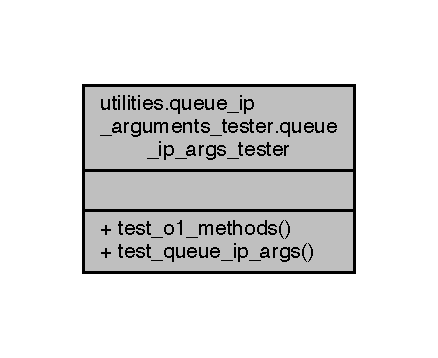
\includegraphics[width=210pt]{d0/dd1/classutilities_1_1queue__ip__arguments__tester_1_1queue__ip__args__tester__coll__graph}
\end{center}
\end{figure}
\subsection*{Static Public Member Functions}
\begin{DoxyCompactItemize}
\item 
def \hyperlink{classutilities_1_1queue__ip__arguments__tester_1_1queue__ip__args__tester_a49bd049dbf616cc1f604d3c0cbe84c43}{test\+\_\+o1\+\_\+methods} ()
\begin{DoxyCompactList}\small\item\em ========================================================= Method to test the O(1) methods that print information to the standard output, or are accessor methods. \end{DoxyCompactList}\item 
def \hyperlink{classutilities_1_1queue__ip__arguments__tester_1_1queue__ip__args__tester_a4af9d2177916d79d95fc9de5531162af}{test\+\_\+if\+\_\+help\+\_\+needed} ()
\begin{DoxyCompactList}\small\item\em ========================================================= Method to test if the user wants to read the brief user manual. \end{DoxyCompactList}\item 
def \hyperlink{classutilities_1_1queue__ip__arguments__tester_1_1queue__ip__args__tester_a53e53ec2797918a6488b0d75ba437407}{test\+\_\+processing\+\_\+input\+\_\+arguments} ()
\begin{DoxyCompactList}\small\item\em ========================================================= Method to test the processing of the 1st \& 2nd input arguments. \end{DoxyCompactList}\item 
def \hyperlink{classutilities_1_1queue__ip__arguments__tester_1_1queue__ip__args__tester_aee90077323d94238d7f81b23e31207c3}{test\+\_\+queue\+\_\+ip\+\_\+args} ()
\begin{DoxyCompactList}\small\item\em ========================================================= Method to test methods that process input arguments to the software. \end{DoxyCompactList}\end{DoxyCompactItemize}


\subsection{Detailed Description}


Definition at line \hyperlink{queue__ip__arguments__tester_8py_source_l00092}{92} of file \hyperlink{queue__ip__arguments__tester_8py_source}{queue\+\_\+ip\+\_\+arguments\+\_\+tester.\+py}.



\subsection{Member Function Documentation}
\hypertarget{classutilities_1_1queue__ip__arguments__tester_1_1queue__ip__args__tester_a4af9d2177916d79d95fc9de5531162af}{}\index{utilities\+::queue\+\_\+ip\+\_\+arguments\+\_\+tester\+::queue\+\_\+ip\+\_\+args\+\_\+tester@{utilities\+::queue\+\_\+ip\+\_\+arguments\+\_\+tester\+::queue\+\_\+ip\+\_\+args\+\_\+tester}!test\+\_\+if\+\_\+help\+\_\+needed@{test\+\_\+if\+\_\+help\+\_\+needed}}
\index{test\+\_\+if\+\_\+help\+\_\+needed@{test\+\_\+if\+\_\+help\+\_\+needed}!utilities\+::queue\+\_\+ip\+\_\+arguments\+\_\+tester\+::queue\+\_\+ip\+\_\+args\+\_\+tester@{utilities\+::queue\+\_\+ip\+\_\+arguments\+\_\+tester\+::queue\+\_\+ip\+\_\+args\+\_\+tester}}
\subsubsection[{test\+\_\+if\+\_\+help\+\_\+needed()}]{\setlength{\rightskip}{0pt plus 5cm}def utilities.\+queue\+\_\+ip\+\_\+arguments\+\_\+tester.\+queue\+\_\+ip\+\_\+args\+\_\+tester.\+test\+\_\+if\+\_\+help\+\_\+needed (
\begin{DoxyParamCaption}
{}
\end{DoxyParamCaption}
)\hspace{0.3cm}{\ttfamily [static]}}\label{classutilities_1_1queue__ip__arguments__tester_1_1queue__ip__args__tester_a4af9d2177916d79d95fc9de5531162af}


========================================================= Method to test if the user wants to read the brief user manual. 

\begin{DoxyReturn}{Returns}
-\/ Nothing. O(1) method. 
\end{DoxyReturn}


Definition at line \hyperlink{queue__ip__arguments__tester_8py_source_l00263}{263} of file \hyperlink{queue__ip__arguments__tester_8py_source}{queue\+\_\+ip\+\_\+arguments\+\_\+tester.\+py}.


\begin{DoxyCode}
\hypertarget{classutilities_1_1queue__ip__arguments__tester_1_1queue__ip__args__tester_l00263}{}\hyperlink{classutilities_1_1queue__ip__arguments__tester_1_1queue__ip__args__tester_a4af9d2177916d79d95fc9de5531162af}{00263}     \textcolor{keyword}{def }\hyperlink{classutilities_1_1queue__ip__arguments__tester_1_1queue__ip__args__tester_a4af9d2177916d79d95fc9de5531162af}{test\_if\_help\_needed}():
00264         print(\textcolor{stringliteral}{" Testing for no help needed..."})
00265         \textcolor{comment}{#   Set the list of input arguments to have 2 arguments.}
00266         name\_of\_script\_dumped = \textcolor{stringliteral}{"name-of-the-script"}
00267         current\_1st\_ip\_arg = \textcolor{stringliteral}{"garbage.json"}
00268         current\_2nd\_ip\_arg = \textcolor{stringliteral}{"nonsense.json"}
00269         new\_list\_ip\_args = [name\_of\_script\_dumped, current\_1st\_ip\_arg, current\_2nd\_ip\_arg]
00270         \textcolor{comment}{#   Assign input arguments to "set\_input\_arguments(...)" for processing.}
00271         queue\_ip\_args.set\_input\_arguments(new\_list\_ip\_args)
00272         prompt8 = \textcolor{stringliteral}{" ... Test: queue\_ip\_args.check\_if\_help\_wanted()  \{\}"}
00273         statistical\_analysis.increment\_number\_test\_cases\_used()
00274         queue\_ip\_args.check\_if\_help\_wanted()
00275         print(prompt8 .format(\textcolor{stringliteral}{" OK"}))
00276         statistical\_analysis.increment\_number\_test\_cases\_passed()
00277         print(\textcolor{stringliteral}{" Testing for help needed (1st arg)... "})
00278         \textcolor{comment}{#   Change the list of input arguments to have "-h" option.}
00279         current\_1st\_ip\_arg = \textcolor{stringliteral}{"-h"}
00280         new\_list\_ip\_args = [name\_of\_script\_dumped, current\_1st\_ip\_arg, current\_2nd\_ip\_arg]
00281         \textcolor{comment}{#   Assign input arguments to "set\_input\_arguments(...)" for processing.}
00282         queue\_ip\_args.set\_input\_arguments(new\_list\_ip\_args)
00283         statistical\_analysis.increment\_number\_test\_cases\_used()
00284         \textcolor{keywordflow}{try}:
00285             queue\_ip\_args.check\_if\_help\_wanted()
00286             print(prompt8 .format(\textcolor{stringliteral}{"FAIL!!!"}))
00287         \textcolor{keywordflow}{except}:
00288             print(prompt8 .format(\textcolor{stringliteral}{" OK"}))
00289             statistical\_analysis.increment\_number\_test\_cases\_passed()
00290         print(\textcolor{stringliteral}{" Testing for help needed (2nd arg)... "})
00291         current\_1st\_ip\_arg = \textcolor{stringliteral}{"garbage.json"}
00292         current\_2nd\_ip\_arg = \textcolor{stringliteral}{"-h"}
00293         new\_list\_ip\_args = [name\_of\_script\_dumped, current\_1st\_ip\_arg, current\_2nd\_ip\_arg]
00294         \textcolor{comment}{#   Assign input arguments to "set\_input\_arguments(...)" for processing.}
00295         queue\_ip\_args.set\_input\_arguments(new\_list\_ip\_args)
00296         statistical\_analysis.increment\_number\_test\_cases\_used()
00297         \textcolor{keywordflow}{try}:
00298             queue\_ip\_args.check\_if\_help\_wanted()
00299             print(prompt8 .format(\textcolor{stringliteral}{"FAIL!!!"}))
00300         \textcolor{keywordflow}{except}:
00301             print(prompt8 .format(\textcolor{stringliteral}{" OK"}))
00302             statistical\_analysis.increment\_number\_test\_cases\_passed()
00303         print(\textcolor{stringliteral}{" Testing for help needed (3rd arg)... "})
00304         current\_1st\_ip\_arg = \textcolor{stringliteral}{"garbage.json"}
00305         current\_2nd\_ip\_arg = \textcolor{stringliteral}{"nonsense.json"}
00306         current\_3rd\_ip\_arg = \textcolor{stringliteral}{"-h"}
00307         new\_list\_ip\_args = [name\_of\_script\_dumped, current\_1st\_ip\_arg, current\_2nd\_ip\_arg, 
      current\_3rd\_ip\_arg]
00308         \textcolor{comment}{#   Assign input arguments to "set\_input\_arguments(...)" for processing.}
00309         queue\_ip\_args.set\_input\_arguments(new\_list\_ip\_args)
00310         statistical\_analysis.increment\_number\_test\_cases\_used()
00311         \textcolor{keywordflow}{try}:
00312             queue\_ip\_args.check\_if\_help\_wanted()
00313             print(prompt8 .format(\textcolor{stringliteral}{"FAIL!!!"}))
00314         \textcolor{keywordflow}{except}:
00315             print(prompt8 .format(\textcolor{stringliteral}{" OK"}))
00316             statistical\_analysis.increment\_number\_test\_cases\_passed()
\end{DoxyCode}
\hypertarget{classutilities_1_1queue__ip__arguments__tester_1_1queue__ip__args__tester_a49bd049dbf616cc1f604d3c0cbe84c43}{}\index{utilities\+::queue\+\_\+ip\+\_\+arguments\+\_\+tester\+::queue\+\_\+ip\+\_\+args\+\_\+tester@{utilities\+::queue\+\_\+ip\+\_\+arguments\+\_\+tester\+::queue\+\_\+ip\+\_\+args\+\_\+tester}!test\+\_\+o1\+\_\+methods@{test\+\_\+o1\+\_\+methods}}
\index{test\+\_\+o1\+\_\+methods@{test\+\_\+o1\+\_\+methods}!utilities\+::queue\+\_\+ip\+\_\+arguments\+\_\+tester\+::queue\+\_\+ip\+\_\+args\+\_\+tester@{utilities\+::queue\+\_\+ip\+\_\+arguments\+\_\+tester\+::queue\+\_\+ip\+\_\+args\+\_\+tester}}
\subsubsection[{test\+\_\+o1\+\_\+methods()}]{\setlength{\rightskip}{0pt plus 5cm}def utilities.\+queue\+\_\+ip\+\_\+arguments\+\_\+tester.\+queue\+\_\+ip\+\_\+args\+\_\+tester.\+test\+\_\+o1\+\_\+methods (
\begin{DoxyParamCaption}
{}
\end{DoxyParamCaption}
)\hspace{0.3cm}{\ttfamily [static]}}\label{classutilities_1_1queue__ip__arguments__tester_1_1queue__ip__args__tester_a49bd049dbf616cc1f604d3c0cbe84c43}


========================================================= Method to test the O(1) methods that print information to the standard output, or are accessor methods. 

\begin{DoxyReturn}{Returns}
-\/ Nothing. O(1) method. O(n) in terms of the number of input arguments. 
\end{DoxyReturn}


Definition at line \hyperlink{queue__ip__arguments__tester_8py_source_l00100}{100} of file \hyperlink{queue__ip__arguments__tester_8py_source}{queue\+\_\+ip\+\_\+arguments\+\_\+tester.\+py}.


\begin{DoxyCode}
\hypertarget{classutilities_1_1queue__ip__arguments__tester_1_1queue__ip__args__tester_l00100}{}\hyperlink{classutilities_1_1queue__ip__arguments__tester_1_1queue__ip__args__tester_a49bd049dbf616cc1f604d3c0cbe84c43}{00100}     \textcolor{keyword}{def }\hyperlink{classutilities_1_1queue__ip__arguments__tester_1_1queue__ip__args__tester_a49bd049dbf616cc1f604d3c0cbe84c43}{test\_o1\_methods}():
00101         print(\textcolor{stringliteral}{" Test: queue\_ip\_args.how\_to\_use\_script()         OK"})
00102         queue\_ip\_args.how\_to\_use\_script()
00103         statistical\_analysis.increment\_number\_test\_cases\_used()
00104         statistical\_analysis.increment\_number\_test\_cases\_passed()
00105         print(\textcolor{stringliteral}{" Test: queue\_ip\_args.print\_help\_option()         OK"})
00106         queue\_ip\_args.print\_help\_option()
00107         statistical\_analysis.increment\_number\_test\_cases\_used()
00108         statistical\_analysis.increment\_number\_test\_cases\_passed()
00109         print(\textcolor{stringliteral}{" Test: queue\_ip\_args.get\_list\_of\_input\_arguments()   OK"})
00110         temp\_set\_ip\_args = queue\_ip\_args.get\_list\_of\_input\_arguments()
00111         statistical\_analysis.increment\_number\_test\_cases\_used()
00112         statistical\_analysis.increment\_number\_test\_cases\_passed()
00113         \textcolor{comment}{#   -   -   -   -   -   -   -   -   -   -   -   -   -   -   -}
00114         print(\textcolor{stringliteral}{" Test: queue\_ip\_args.print\_all\_input\_arguments()     OK"})
00115         queue\_ip\_args.print\_all\_input\_arguments()
00116         statistical\_analysis.increment\_number\_test\_cases\_used()
00117         statistical\_analysis.increment\_number\_test\_cases\_passed()
00118         \textcolor{comment}{#   -   -   -   -   -   -   -   -   -   -   -   -   -   -   -}
00119         prompt = \textcolor{stringliteral}{"  Test: queue\_ip\_args.get\_1st\_input\_argument()        \{\}"}
00120         statistical\_analysis.increment\_number\_test\_cases\_used()
00121         \textcolor{keywordflow}{if} queue\_ip\_args.get\_1st\_input\_argument() \textcolor{keywordflow}{is} \textcolor{keywordflow}{not} \textcolor{keywordtype}{None}:
00122             print(prompt .format(\textcolor{stringliteral}{"OK"}))
00123             statistical\_analysis.increment\_number\_test\_cases\_passed()
00124         \textcolor{keywordflow}{else}:
00125             print(prompt .format(\textcolor{stringliteral}{"FAIL!!!"}))
00126         \textcolor{comment}{#   -   -   -   -   -   -   -   -   -   -   -   -   -   -   -}
00127         prompt = \textcolor{stringliteral}{"  Test: queue\_ip\_args.get\_2nd\_input\_argument()        \{\}"}
00128         statistical\_analysis.increment\_number\_test\_cases\_used()
00129         \textcolor{keywordflow}{if} queue\_ip\_args.get\_2nd\_input\_argument() \textcolor{keywordflow}{is} \textcolor{keywordflow}{not} \textcolor{keywordtype}{None}:
00130             print(prompt .format(\textcolor{stringliteral}{"OK"}))
00131             statistical\_analysis.increment\_number\_test\_cases\_passed()
00132         \textcolor{keywordflow}{else}:
00133             print(prompt .format(\textcolor{stringliteral}{"FAIL!!!"}))
00134         \textcolor{comment}{#   -   -   -   -   -   -   -   -   -   -   -   -   -   -   -}
00135         print(\textcolor{stringliteral}{" Testing for an empty list..."})
00136         prompt1 = \textcolor{stringliteral}{" ... Test: queue\_ip\_args.get\_list\_of\_input\_arguments()   \{\}"}
00137         statistical\_analysis.increment\_number\_test\_cases\_used()
00138         prompt2 = \textcolor{stringliteral}{" ... Test: queue\_ip\_args.get\_number\_of\_input\_arguments() \{\}"}
00139         statistical\_analysis.increment\_number\_test\_cases\_used()
00140         prompt4 = \textcolor{stringliteral}{" ... Test: queue\_ip\_args.set\_input\_arguments(...)    \{\}"}
00141         statistical\_analysis.increment\_number\_test\_cases\_used()
00142         prompt5 = \textcolor{stringliteral}{" ... Test: queue\_ip\_args.get\_1st\_input\_argument()    \{\}"}
00143         prompt6 = \textcolor{stringliteral}{" ... Test: queue\_ip\_args.get\_2nd\_input\_argument()    \{\}"}
00144         \textcolor{comment}{#   List of input arguments.}
00145         old\_list\_ip\_args = queue\_ip\_args.get\_list\_of\_input\_arguments()
00146         new\_list\_ip\_args = []
00147         \textcolor{stringliteral}{"""}
00148 \textcolor{stringliteral}{            Assign input arguments to "set\_input\_arguments(...)" for}
00149 \textcolor{stringliteral}{                processing.}
00150 \textcolor{stringliteral}{            Statement should fail.}
00151 \textcolor{stringliteral}{        """}
00152         \textcolor{keywordflow}{try}:
00153             queue\_ip\_args.set\_input\_arguments(new\_list\_ip\_args)
00154         \textcolor{keywordflow}{except}:
00155             \textcolor{keywordflow}{if} old\_list\_ip\_args == queue\_ip\_args.get\_list\_of\_input\_arguments():
00156                 print(prompt1 .format(\textcolor{stringliteral}{"OK"}))
00157                 statistical\_analysis.increment\_number\_test\_cases\_passed()
00158             \textcolor{keywordflow}{else}:
00159                 print(prompt1 .format(\textcolor{stringliteral}{"FAIL!!!"}))
00160                 \textcolor{comment}{#print(queue\_ip\_args.get\_list\_of\_input\_arguments())}
00161             \textcolor{keywordflow}{if} len(old\_list\_ip\_args) == queue\_ip\_args.get\_number\_of\_input\_arguments():
00162                 print(prompt2 .format(\textcolor{stringliteral}{"OK"}))
00163                 statistical\_analysis.increment\_number\_test\_cases\_passed()
00164             \textcolor{keywordflow}{else}:
00165                 print(prompt2 .format(\textcolor{stringliteral}{"FAIL!!!"}))
00166                 \textcolor{comment}{#print(queue\_ip\_args.get\_number\_of\_input\_arguments())}
00167             print(prompt4 .format(\textcolor{stringliteral}{"OK"}))
00168             statistical\_analysis.increment\_number\_test\_cases\_passed()
00169         print(\textcolor{stringliteral}{" Testing for list with 1 argument..."})
00170         \textcolor{stringliteral}{"""}
00171 \textcolor{stringliteral}{            Set the list of input arguments to have 1 argument, in addition}
00172 \textcolor{stringliteral}{                to the name of the script.}
00173 \textcolor{stringliteral}{            Hence, the list would have 2 arguments, since the first}
00174 \textcolor{stringliteral}{                "argument" is dumped during the method call to}
00175 \textcolor{stringliteral}{                set\_input\_arguments(...);}
00176 \textcolor{stringliteral}{                this first "argument" is the name of the currently executing}
00177 \textcolor{stringliteral}{                    script.}
00178 \textcolor{stringliteral}{        """}
00179         name\_of\_script\_dumped = \textcolor{stringliteral}{"name-of-the-script"}
00180         current\_1st\_ip\_arg = \textcolor{stringliteral}{"benchmarks/majority\_netlist.json"}
00181         new\_list\_ip\_args = [name\_of\_script\_dumped, current\_1st\_ip\_arg]
00182         \textcolor{comment}{#   Assign input arguments to "set\_input\_arguments(...)" for processing.}
00183         queue\_ip\_args.set\_input\_arguments(new\_list\_ip\_args)
00184         statistical\_analysis.increment\_number\_test\_cases\_used()
00185         \textcolor{keywordflow}{if} new\_list\_ip\_args == queue\_ip\_args.get\_list\_of\_input\_arguments():
00186             print(prompt1 .format(\textcolor{stringliteral}{"OK"}))
00187             statistical\_analysis.increment\_number\_test\_cases\_passed()
00188         \textcolor{keywordflow}{else}:
00189             print(prompt1 .format(\textcolor{stringliteral}{"FAIL!!!"}))
00190             \textcolor{comment}{#print(queue\_ip\_args.get\_list\_of\_input\_arguments())}
00191         statistical\_analysis.increment\_number\_test\_cases\_used()
00192         \textcolor{keywordflow}{if} len(new\_list\_ip\_args) == queue\_ip\_args.get\_number\_of\_input\_arguments():
00193             print(prompt2 .format(\textcolor{stringliteral}{"OK"}))
00194             statistical\_analysis.increment\_number\_test\_cases\_passed()
00195         \textcolor{keywordflow}{else}:
00196             print(prompt2 .format(\textcolor{stringliteral}{"FAIL!!!"}))
00197             \textcolor{comment}{#print(len(new\_list\_ip\_args)-1)}
00198             \textcolor{comment}{#print(queue\_ip\_args.get\_number\_of\_input\_arguments())}
00199         statistical\_analysis.increment\_number\_test\_cases\_used()
00200         print(prompt4 .format(\textcolor{stringliteral}{"OK"}))
00201         statistical\_analysis.increment\_number\_test\_cases\_passed()
00202         \textcolor{comment}{#   -   -   -   -   -   -   -   -   -   -   -   -   -   -}
00203         statistical\_analysis.increment\_number\_test\_cases\_used()
00204         \textcolor{keywordflow}{if} current\_1st\_ip\_arg == queue\_ip\_args.get\_1st\_input\_argument():
00205             print(prompt5 .format(\textcolor{stringliteral}{"OK"}))
00206             statistical\_analysis.increment\_number\_test\_cases\_passed()
00207         \textcolor{keywordflow}{else}:
00208             print(prompt5 .format(\textcolor{stringliteral}{"FAIL!!!"}))
00209         \textcolor{stringliteral}{"""}
00210 \textcolor{stringliteral}{            If an input argument for the software is "-h", show the}
00211 \textcolor{stringliteral}{                brief user manual to the user.}
00212 \textcolor{stringliteral}{            Else, there is no need to test for more than 2 input arguments}
00213 \textcolor{stringliteral}{                for the software, since only the first two are processed.}
00214 \textcolor{stringliteral}{            So, the list shall have 3 elements, since the first element}
00215 \textcolor{stringliteral}{                is dumped during the method call to set\_input\_arguments(...).}
00216 \textcolor{stringliteral}{        """}
00217         print(\textcolor{stringliteral}{" Testing for list with 2 arguments..."})
00218         \textcolor{comment}{#   Set the list of input arguments to have 2 arguments.}
00219         \textcolor{comment}{#new\_list\_ip\_args = ["benchmarks/majority\_netlist.json" "nonsense.json"]}
00220         current\_1st\_ip\_arg = \textcolor{stringliteral}{"garbage.json"}
00221         current\_2nd\_ip\_arg = \textcolor{stringliteral}{"nonsense.json"}
00222         new\_list\_ip\_args = [name\_of\_script\_dumped, current\_1st\_ip\_arg, current\_2nd\_ip\_arg]
00223         \textcolor{comment}{#   Assign input arguments to "set\_input\_arguments(...)" for processing.}
00224         queue\_ip\_args.set\_input\_arguments(new\_list\_ip\_args)
00225         statistical\_analysis.increment\_number\_test\_cases\_used()
00226         \textcolor{keywordflow}{if} new\_list\_ip\_args == queue\_ip\_args.get\_list\_of\_input\_arguments():
00227             print(prompt1 .format(\textcolor{stringliteral}{"OK"}))
00228             statistical\_analysis.increment\_number\_test\_cases\_passed()
00229         \textcolor{keywordflow}{else}:
00230             print(prompt1 .format(\textcolor{stringliteral}{"FAIL!!!"}))
00231             \textcolor{comment}{#print(queue\_ip\_args.get\_list\_of\_input\_arguments())}
00232         statistical\_analysis.increment\_number\_test\_cases\_used()
00233         \textcolor{keywordflow}{if} len(new\_list\_ip\_args) == queue\_ip\_args.get\_number\_of\_input\_arguments():
00234             print(prompt2 .format(\textcolor{stringliteral}{"OK"}))
00235             statistical\_analysis.increment\_number\_test\_cases\_passed()
00236         \textcolor{keywordflow}{else}:
00237             print(prompt2 .format(\textcolor{stringliteral}{"FAIL!!!"}))
00238             \textcolor{comment}{#print(queue\_ip\_args.get\_number\_of\_input\_arguments())}
00239         statistical\_analysis.increment\_number\_test\_cases\_used()
00240         print(prompt4 .format(\textcolor{stringliteral}{"OK"}))
00241         statistical\_analysis.increment\_number\_test\_cases\_passed()
00242         \textcolor{comment}{#   -   -   -   -   -   -   -   -   -   -   -   -   -   -}
00243         statistical\_analysis.increment\_number\_test\_cases\_used()
00244         \textcolor{keywordflow}{if} current\_2nd\_ip\_arg == queue\_ip\_args.get\_2nd\_input\_argument():
00245             print(prompt6 .format(\textcolor{stringliteral}{"OK"}))
00246             statistical\_analysis.increment\_number\_test\_cases\_passed()
00247         \textcolor{keywordflow}{else}:
00248             print(prompt6 .format(\textcolor{stringliteral}{"FAIL!!!"}))
00249         prompt7 = \textcolor{stringliteral}{" ... Test: queue\_ip\_args.input\_arguments\_error() \{\}"}
00250         statistical\_analysis.increment\_number\_test\_cases\_used()
00251         \textcolor{keywordflow}{try}:
00252             queue\_ip\_args.input\_arguments\_error()
00253             print(prompt7 .format(\textcolor{stringliteral}{"FAIL!!!"}))
00254         \textcolor{keywordflow}{except}:
00255             print(prompt7 .format(\textcolor{stringliteral}{" OK"}))
00256             statistical\_analysis.increment\_number\_test\_cases\_passed()
\end{DoxyCode}
\hypertarget{classutilities_1_1queue__ip__arguments__tester_1_1queue__ip__args__tester_a53e53ec2797918a6488b0d75ba437407}{}\index{utilities\+::queue\+\_\+ip\+\_\+arguments\+\_\+tester\+::queue\+\_\+ip\+\_\+args\+\_\+tester@{utilities\+::queue\+\_\+ip\+\_\+arguments\+\_\+tester\+::queue\+\_\+ip\+\_\+args\+\_\+tester}!test\+\_\+processing\+\_\+input\+\_\+arguments@{test\+\_\+processing\+\_\+input\+\_\+arguments}}
\index{test\+\_\+processing\+\_\+input\+\_\+arguments@{test\+\_\+processing\+\_\+input\+\_\+arguments}!utilities\+::queue\+\_\+ip\+\_\+arguments\+\_\+tester\+::queue\+\_\+ip\+\_\+args\+\_\+tester@{utilities\+::queue\+\_\+ip\+\_\+arguments\+\_\+tester\+::queue\+\_\+ip\+\_\+args\+\_\+tester}}
\subsubsection[{test\+\_\+processing\+\_\+input\+\_\+arguments()}]{\setlength{\rightskip}{0pt plus 5cm}def utilities.\+queue\+\_\+ip\+\_\+arguments\+\_\+tester.\+queue\+\_\+ip\+\_\+args\+\_\+tester.\+test\+\_\+processing\+\_\+input\+\_\+arguments (
\begin{DoxyParamCaption}
{}
\end{DoxyParamCaption}
)\hspace{0.3cm}{\ttfamily [static]}}\label{classutilities_1_1queue__ip__arguments__tester_1_1queue__ip__args__tester_a53e53ec2797918a6488b0d75ba437407}


========================================================= Method to test the processing of the 1st \& 2nd input arguments. 

\begin{DoxyReturn}{Returns}
-\/ Nothing. O(1) method. 
\end{DoxyReturn}


Definition at line \hyperlink{queue__ip__arguments__tester_8py_source_l00322}{322} of file \hyperlink{queue__ip__arguments__tester_8py_source}{queue\+\_\+ip\+\_\+arguments\+\_\+tester.\+py}.


\begin{DoxyCode}
\hypertarget{classutilities_1_1queue__ip__arguments__tester_1_1queue__ip__args__tester_l00322}{}\hyperlink{classutilities_1_1queue__ip__arguments__tester_1_1queue__ip__args__tester_a53e53ec2797918a6488b0d75ba437407}{00322}     \textcolor{keyword}{def }\hyperlink{classutilities_1_1queue__ip__arguments__tester_1_1queue__ip__args__tester_a53e53ec2797918a6488b0d75ba437407}{test\_processing\_input\_arguments}():
00323         print(\textcolor{stringliteral}{" Test: queue\_ip\_args.process\_1st\_ip\_arg()... "})
00324         name\_of\_script\_dumped = \textcolor{stringliteral}{"name-of-the-script"}
00325         current\_1st\_ip\_arg = \textcolor{stringliteral}{"garbage.json"}
00326         current\_2nd\_ip\_arg = \textcolor{stringliteral}{"notes/guidelines/guidelines.tex"}
00327         new\_list\_ip\_args = [name\_of\_script\_dumped, current\_1st\_ip\_arg, current\_2nd\_ip\_arg]
00328         \textcolor{comment}{#   Assign input arguments to "set\_input\_arguments(...)" for processing.}
00329         queue\_ip\_args.set\_input\_arguments(new\_list\_ip\_args)
00330         prompt9 = \textcolor{stringliteral}{" ... Invalid path to file    \{\}"}
00331         statistical\_analysis.increment\_number\_test\_cases\_used()
00332         \textcolor{keywordflow}{try}:
00333             ip\_fname = queue\_ip\_args.process\_1st\_ip\_arg()
00334             print(prompt9 .format(\textcolor{stringliteral}{"     FAIL!!!"}))
00335         \textcolor{keywordflow}{except}:
00336             print(prompt9 .format(\textcolor{stringliteral}{"         OK"}))
00337             statistical\_analysis.increment\_number\_test\_cases\_passed()
00338         \textcolor{comment}{#   -   -   -   -   -   -   -   -   -   -   -   -   -}
00339         \textcolor{stringliteral}{"""}
00340 \textcolor{stringliteral}{            1st input argument: Valid path to file, no JSON file extension.}
00341 \textcolor{stringliteral}{        """}
00342         \textcolor{comment}{#current\_1st\_ip\_arg = "benchmarks/majority\_netlist.json"}
00343         current\_1st\_ip\_arg = \textcolor{stringliteral}{"notes/mit-license.text"}
00344         new\_list\_ip\_args = [name\_of\_script\_dumped, current\_1st\_ip\_arg, current\_2nd\_ip\_arg]
00345         queue\_ip\_args.set\_input\_arguments(new\_list\_ip\_args)
00346         prompt10 = \textcolor{stringliteral}{"    ... Valid path to file, no JSON file extension. \{\}"}
00347         statistical\_analysis.increment\_number\_test\_cases\_used()
00348         \textcolor{keywordflow}{try}:
00349             ip\_fname = queue\_ip\_args.process\_1st\_ip\_arg()
00350             print(prompt10 .format(\textcolor{stringliteral}{"        FAIL!!!"}))
00351         \textcolor{keywordflow}{except}:
00352             print(prompt10 .format(\textcolor{stringliteral}{"    OK"}))
00353             statistical\_analysis.increment\_number\_test\_cases\_passed()
00354         \textcolor{stringliteral}{"""}
00355 \textcolor{stringliteral}{            1st input argument: Valid path to file, JSON file extension.}
00356 \textcolor{stringliteral}{        """}
00357         current\_1st\_ip\_arg = \textcolor{stringliteral}{"benchmarks/majority\_netlist.json"}
00358         new\_list\_ip\_args = [name\_of\_script\_dumped, current\_1st\_ip\_arg, current\_2nd\_ip\_arg]
00359         queue\_ip\_args.set\_input\_arguments(new\_list\_ip\_args)
00360         prompt10 = \textcolor{stringliteral}{"    ... Valid path to file, JSON file extension.    \{\}"}
00361         statistical\_analysis.increment\_number\_test\_cases\_used()
00362         ip\_fname = queue\_ip\_args.process\_1st\_ip\_arg()
00363         print(prompt10 .format(\textcolor{stringliteral}{"    OK"}))
00364         statistical\_analysis.increment\_number\_test\_cases\_passed()
00365         print(\textcolor{stringliteral}{" -   -   -   -   -   -   -   -"})
00366         print(\textcolor{stringliteral}{" Test: queue\_ip\_args.process\_2nd\_ip\_arg()... "})
00367         prompt11 = \textcolor{stringliteral}{"    ... Valid path to file  \{\}"}
00368         statistical\_analysis.increment\_number\_test\_cases\_used()
00369         \textcolor{keywordflow}{try}:
00370             op\_fname = queue\_ip\_args.process\_2nd\_ip\_arg()
00371             print(prompt11 .format(\textcolor{stringliteral}{"                FAIL!!!"}))
00372         \textcolor{keywordflow}{except}:
00373             print(prompt11 .format(\textcolor{stringliteral}{"                OK"}))
00374             statistical\_analysis.increment\_number\_test\_cases\_passed()
00375         prompt12 = \textcolor{stringliteral}{"    ... Invalid path to file, no JSON extension \{\}"}
00376         statistical\_analysis.increment\_number\_test\_cases\_used()
00377         current\_2nd\_ip\_arg = \textcolor{stringliteral}{"nonsense"}
00378         new\_list\_ip\_args = [name\_of\_script\_dumped, current\_1st\_ip\_arg, current\_2nd\_ip\_arg]
00379         queue\_ip\_args.set\_input\_arguments(new\_list\_ip\_args)
00380         \textcolor{keywordflow}{try}:
00381             op\_fname = queue\_ip\_args.process\_2nd\_ip\_arg()
00382             print(prompt12 .format(\textcolor{stringliteral}{"    OK"}))
00383             statistical\_analysis.increment\_number\_test\_cases\_passed()
00384         \textcolor{keywordflow}{except}:
00385             print(prompt12 .format(\textcolor{stringliteral}{"    FAIL!!!"}))
00386         prompt13 = \textcolor{stringliteral}{"    ... Invalid path to file, JSON extension    \{\}"}
00387         statistical\_analysis.increment\_number\_test\_cases\_used()
00388         current\_2nd\_ip\_arg = \textcolor{stringliteral}{"nonsense.json"}
00389         new\_list\_ip\_args = [name\_of\_script\_dumped, current\_1st\_ip\_arg, current\_2nd\_ip\_arg]
00390         queue\_ip\_args.set\_input\_arguments(new\_list\_ip\_args)
00391         \textcolor{keywordflow}{try}:
00392             op\_fname = queue\_ip\_args.process\_2nd\_ip\_arg()
00393             print(prompt13 .format(\textcolor{stringliteral}{"    OK"}))
00394             statistical\_analysis.increment\_number\_test\_cases\_passed()
00395         \textcolor{keywordflow}{except}:
00396             print(prompt13 .format(\textcolor{stringliteral}{"    FAIL!!!"}))
00397 
\end{DoxyCode}
\hypertarget{classutilities_1_1queue__ip__arguments__tester_1_1queue__ip__args__tester_aee90077323d94238d7f81b23e31207c3}{}\index{utilities\+::queue\+\_\+ip\+\_\+arguments\+\_\+tester\+::queue\+\_\+ip\+\_\+args\+\_\+tester@{utilities\+::queue\+\_\+ip\+\_\+arguments\+\_\+tester\+::queue\+\_\+ip\+\_\+args\+\_\+tester}!test\+\_\+queue\+\_\+ip\+\_\+args@{test\+\_\+queue\+\_\+ip\+\_\+args}}
\index{test\+\_\+queue\+\_\+ip\+\_\+args@{test\+\_\+queue\+\_\+ip\+\_\+args}!utilities\+::queue\+\_\+ip\+\_\+arguments\+\_\+tester\+::queue\+\_\+ip\+\_\+args\+\_\+tester@{utilities\+::queue\+\_\+ip\+\_\+arguments\+\_\+tester\+::queue\+\_\+ip\+\_\+args\+\_\+tester}}
\subsubsection[{test\+\_\+queue\+\_\+ip\+\_\+args()}]{\setlength{\rightskip}{0pt plus 5cm}def utilities.\+queue\+\_\+ip\+\_\+arguments\+\_\+tester.\+queue\+\_\+ip\+\_\+args\+\_\+tester.\+test\+\_\+queue\+\_\+ip\+\_\+args (
\begin{DoxyParamCaption}
{}
\end{DoxyParamCaption}
)\hspace{0.3cm}{\ttfamily [static]}}\label{classutilities_1_1queue__ip__arguments__tester_1_1queue__ip__args__tester_aee90077323d94238d7f81b23e31207c3}


========================================================= Method to test methods that process input arguments to the software. 

\begin{DoxyReturn}{Returns}
-\/ Nothing. O(1) method. 
\end{DoxyReturn}


Definition at line \hyperlink{queue__ip__arguments__tester_8py_source_l00404}{404} of file \hyperlink{queue__ip__arguments__tester_8py_source}{queue\+\_\+ip\+\_\+arguments\+\_\+tester.\+py}.


\begin{DoxyCode}
\hypertarget{classutilities_1_1queue__ip__arguments__tester_1_1queue__ip__args__tester_l00404}{}\hyperlink{classutilities_1_1queue__ip__arguments__tester_1_1queue__ip__args__tester_aee90077323d94238d7f81b23e31207c3}{00404}     \textcolor{keyword}{def }\hyperlink{classutilities_1_1queue__ip__arguments__tester_1_1queue__ip__args__tester_aee90077323d94238d7f81b23e31207c3}{test\_queue\_ip\_args}():
00405         print(\textcolor{stringliteral}{"==   Testing class: queue\_ip\_args."})
00406         queue\_ip\_args\_tester.test\_o1\_methods()
00407         queue\_ip\_args\_tester.test\_if\_help\_needed()
00408         queue\_ip\_args\_tester.test\_processing\_input\_arguments()
00409 \end{DoxyCode}


The documentation for this class was generated from the following file\+:\begin{DoxyCompactItemize}
\item 
utilities/\hyperlink{queue__ip__arguments__tester_8py}{queue\+\_\+ip\+\_\+arguments\+\_\+tester.\+py}\end{DoxyCompactItemize}

\hypertarget{classstatistics_1_1test__statistics_1_1statistical__analysis}{}\section{statistics.\+test\+\_\+statistics.\+statistical\+\_\+analysis Class Reference}
\label{classstatistics_1_1test__statistics_1_1statistical__analysis}\index{statistics.\+test\+\_\+statistics.\+statistical\+\_\+analysis@{statistics.\+test\+\_\+statistics.\+statistical\+\_\+analysis}}


Import Custom Python Modules.  




Collaboration diagram for statistics.\+test\+\_\+statistics.\+statistical\+\_\+analysis\+:
\nopagebreak
\begin{figure}[H]
\begin{center}
\leavevmode
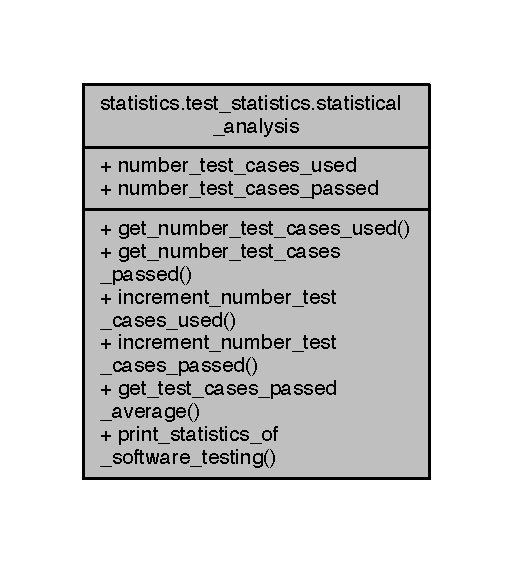
\includegraphics[width=246pt]{dd/d6c/classstatistics_1_1test__statistics_1_1statistical__analysis__coll__graph}
\end{center}
\end{figure}
\subsection*{Static Public Member Functions}
\begin{DoxyCompactItemize}
\item 
def \hyperlink{classstatistics_1_1test__statistics_1_1statistical__analysis_a8bddd92400d64e68caf934defa5ededb}{get\+\_\+number\+\_\+test\+\_\+cases\+\_\+used} ()
\item 
def \hyperlink{classstatistics_1_1test__statistics_1_1statistical__analysis_a0461b276e37fd6c24ab919efbeb04309}{get\+\_\+number\+\_\+test\+\_\+cases\+\_\+passed} ()
\item 
def \hyperlink{classstatistics_1_1test__statistics_1_1statistical__analysis_a7e88e87c8e6739dcaa37740985089f11}{increment\+\_\+number\+\_\+test\+\_\+cases\+\_\+used} ()
\item 
def \hyperlink{classstatistics_1_1test__statistics_1_1statistical__analysis_a056f55c0e7f60e29d4b37e8e74d3cd08}{increment\+\_\+number\+\_\+test\+\_\+cases\+\_\+passed} ()
\item 
def \hyperlink{classstatistics_1_1test__statistics_1_1statistical__analysis_a1bec04d2404b2bdf277c4ba170abb4a1}{get\+\_\+test\+\_\+cases\+\_\+passed\+\_\+average} ()
\item 
def \hyperlink{classstatistics_1_1test__statistics_1_1statistical__analysis_ad6bdf2cde8553974d93d5971870970d8}{print\+\_\+statistics\+\_\+of\+\_\+software\+\_\+testing} ()
\end{DoxyCompactItemize}
\subsection*{Static Public Attributes}
\begin{DoxyCompactItemize}
\item 
int \hyperlink{classstatistics_1_1test__statistics_1_1statistical__analysis_afed7a27a010e7377d2719b315d5d5f17}{number\+\_\+test\+\_\+cases\+\_\+used} = 0
\item 
int \hyperlink{classstatistics_1_1test__statistics_1_1statistical__analysis_ac7555db570919cec38a8325d8427093e}{number\+\_\+test\+\_\+cases\+\_\+passed} = 0
\end{DoxyCompactItemize}


\subsection{Detailed Description}
Import Custom Python Modules. 

Definition at line \hyperlink{test__statistics_8py_source_l00081}{81} of file \hyperlink{test__statistics_8py_source}{test\+\_\+statistics.\+py}.



\subsection{Member Function Documentation}
\hypertarget{classstatistics_1_1test__statistics_1_1statistical__analysis_a0461b276e37fd6c24ab919efbeb04309}{}\index{statistics\+::test\+\_\+statistics\+::statistical\+\_\+analysis@{statistics\+::test\+\_\+statistics\+::statistical\+\_\+analysis}!get\+\_\+number\+\_\+test\+\_\+cases\+\_\+passed@{get\+\_\+number\+\_\+test\+\_\+cases\+\_\+passed}}
\index{get\+\_\+number\+\_\+test\+\_\+cases\+\_\+passed@{get\+\_\+number\+\_\+test\+\_\+cases\+\_\+passed}!statistics\+::test\+\_\+statistics\+::statistical\+\_\+analysis@{statistics\+::test\+\_\+statistics\+::statistical\+\_\+analysis}}
\subsubsection[{get\+\_\+number\+\_\+test\+\_\+cases\+\_\+passed()}]{\setlength{\rightskip}{0pt plus 5cm}def statistics.\+test\+\_\+statistics.\+statistical\+\_\+analysis.\+get\+\_\+number\+\_\+test\+\_\+cases\+\_\+passed (
\begin{DoxyParamCaption}
{}
\end{DoxyParamCaption}
)\hspace{0.3cm}{\ttfamily [static]}}\label{classstatistics_1_1test__statistics_1_1statistical__analysis_a0461b276e37fd6c24ab919efbeb04309}


Definition at line \hyperlink{test__statistics_8py_source_l00104}{104} of file \hyperlink{test__statistics_8py_source}{test\+\_\+statistics.\+py}.


\begin{DoxyCode}
\hypertarget{classstatistics_1_1test__statistics_1_1statistical__analysis_l00104}{}\hyperlink{classstatistics_1_1test__statistics_1_1statistical__analysis_a0461b276e37fd6c24ab919efbeb04309}{00104}     \textcolor{keyword}{def }\hyperlink{classstatistics_1_1test__statistics_1_1statistical__analysis_a0461b276e37fd6c24ab919efbeb04309}{get\_number\_test\_cases\_passed}():
00105         \textcolor{keywordflow}{return} statistical\_analysis.number\_test\_cases\_passed
\end{DoxyCode}
\hypertarget{classstatistics_1_1test__statistics_1_1statistical__analysis_a8bddd92400d64e68caf934defa5ededb}{}\index{statistics\+::test\+\_\+statistics\+::statistical\+\_\+analysis@{statistics\+::test\+\_\+statistics\+::statistical\+\_\+analysis}!get\+\_\+number\+\_\+test\+\_\+cases\+\_\+used@{get\+\_\+number\+\_\+test\+\_\+cases\+\_\+used}}
\index{get\+\_\+number\+\_\+test\+\_\+cases\+\_\+used@{get\+\_\+number\+\_\+test\+\_\+cases\+\_\+used}!statistics\+::test\+\_\+statistics\+::statistical\+\_\+analysis@{statistics\+::test\+\_\+statistics\+::statistical\+\_\+analysis}}
\subsubsection[{get\+\_\+number\+\_\+test\+\_\+cases\+\_\+used()}]{\setlength{\rightskip}{0pt plus 5cm}def statistics.\+test\+\_\+statistics.\+statistical\+\_\+analysis.\+get\+\_\+number\+\_\+test\+\_\+cases\+\_\+used (
\begin{DoxyParamCaption}
{}
\end{DoxyParamCaption}
)\hspace{0.3cm}{\ttfamily [static]}}\label{classstatistics_1_1test__statistics_1_1statistical__analysis_a8bddd92400d64e68caf934defa5ededb}


Definition at line \hyperlink{test__statistics_8py_source_l00096}{96} of file \hyperlink{test__statistics_8py_source}{test\+\_\+statistics.\+py}.


\begin{DoxyCode}
\hypertarget{classstatistics_1_1test__statistics_1_1statistical__analysis_l00096}{}\hyperlink{classstatistics_1_1test__statistics_1_1statistical__analysis_a8bddd92400d64e68caf934defa5ededb}{00096}     \textcolor{keyword}{def }\hyperlink{classstatistics_1_1test__statistics_1_1statistical__analysis_a8bddd92400d64e68caf934defa5ededb}{get\_number\_test\_cases\_used}():
00097         \textcolor{keywordflow}{return} statistical\_analysis.number\_test\_cases\_used
\end{DoxyCode}
\hypertarget{classstatistics_1_1test__statistics_1_1statistical__analysis_a1bec04d2404b2bdf277c4ba170abb4a1}{}\index{statistics\+::test\+\_\+statistics\+::statistical\+\_\+analysis@{statistics\+::test\+\_\+statistics\+::statistical\+\_\+analysis}!get\+\_\+test\+\_\+cases\+\_\+passed\+\_\+average@{get\+\_\+test\+\_\+cases\+\_\+passed\+\_\+average}}
\index{get\+\_\+test\+\_\+cases\+\_\+passed\+\_\+average@{get\+\_\+test\+\_\+cases\+\_\+passed\+\_\+average}!statistics\+::test\+\_\+statistics\+::statistical\+\_\+analysis@{statistics\+::test\+\_\+statistics\+::statistical\+\_\+analysis}}
\subsubsection[{get\+\_\+test\+\_\+cases\+\_\+passed\+\_\+average()}]{\setlength{\rightskip}{0pt plus 5cm}def statistics.\+test\+\_\+statistics.\+statistical\+\_\+analysis.\+get\+\_\+test\+\_\+cases\+\_\+passed\+\_\+average (
\begin{DoxyParamCaption}
{}
\end{DoxyParamCaption}
)\hspace{0.3cm}{\ttfamily [static]}}\label{classstatistics_1_1test__statistics_1_1statistical__analysis_a1bec04d2404b2bdf277c4ba170abb4a1}


Definition at line \hyperlink{test__statistics_8py_source_l00146}{146} of file \hyperlink{test__statistics_8py_source}{test\+\_\+statistics.\+py}.


\begin{DoxyCode}
\hypertarget{classstatistics_1_1test__statistics_1_1statistical__analysis_l00146}{}\hyperlink{classstatistics_1_1test__statistics_1_1statistical__analysis_a1bec04d2404b2bdf277c4ba170abb4a1}{00146}     \textcolor{keyword}{def }\hyperlink{classstatistics_1_1test__statistics_1_1statistical__analysis_a1bec04d2404b2bdf277c4ba170abb4a1}{get\_test\_cases\_passed\_average}():
00147         \textcolor{keywordflow}{if} (statistical\_analysis.number\_test\_cases\_used > statistical\_analysis.number\_test\_cases\_passed):
00148             print(\textcolor{stringliteral}{" Problem: number\_test\_cases\_used > number\_test\_cases\_passed"})
00149             \textcolor{keywordflow}{raise} Exception(\textcolor{stringliteral}{"   Precondition failed (1): see number\_test\_cases\_used or
       number\_test\_cases\_passed."})
00150         \textcolor{keywordflow}{return} (statistical\_analysis.number\_test\_cases\_passed*100 / 
      statistical\_analysis.number\_test\_cases\_used) 
\end{DoxyCode}
\hypertarget{classstatistics_1_1test__statistics_1_1statistical__analysis_a056f55c0e7f60e29d4b37e8e74d3cd08}{}\index{statistics\+::test\+\_\+statistics\+::statistical\+\_\+analysis@{statistics\+::test\+\_\+statistics\+::statistical\+\_\+analysis}!increment\+\_\+number\+\_\+test\+\_\+cases\+\_\+passed@{increment\+\_\+number\+\_\+test\+\_\+cases\+\_\+passed}}
\index{increment\+\_\+number\+\_\+test\+\_\+cases\+\_\+passed@{increment\+\_\+number\+\_\+test\+\_\+cases\+\_\+passed}!statistics\+::test\+\_\+statistics\+::statistical\+\_\+analysis@{statistics\+::test\+\_\+statistics\+::statistical\+\_\+analysis}}
\subsubsection[{increment\+\_\+number\+\_\+test\+\_\+cases\+\_\+passed()}]{\setlength{\rightskip}{0pt plus 5cm}def statistics.\+test\+\_\+statistics.\+statistical\+\_\+analysis.\+increment\+\_\+number\+\_\+test\+\_\+cases\+\_\+passed (
\begin{DoxyParamCaption}
{}
\end{DoxyParamCaption}
)\hspace{0.3cm}{\ttfamily [static]}}\label{classstatistics_1_1test__statistics_1_1statistical__analysis_a056f55c0e7f60e29d4b37e8e74d3cd08}


Definition at line \hyperlink{test__statistics_8py_source_l00128}{128} of file \hyperlink{test__statistics_8py_source}{test\+\_\+statistics.\+py}.


\begin{DoxyCode}
\hypertarget{classstatistics_1_1test__statistics_1_1statistical__analysis_l00128}{}\hyperlink{classstatistics_1_1test__statistics_1_1statistical__analysis_a056f55c0e7f60e29d4b37e8e74d3cd08}{00128}     \textcolor{keyword}{def }\hyperlink{classstatistics_1_1test__statistics_1_1statistical__analysis_a056f55c0e7f60e29d4b37e8e74d3cd08}{increment\_number\_test\_cases\_passed}():
00129         \textcolor{keywordflow}{if} 0 == statistical\_analysis.number\_test\_cases\_passed:
00130             statistical\_analysis.number\_test\_cases\_passed = 1
00131         \textcolor{keywordflow}{else}:
00132             statistical\_analysis.number\_test\_cases\_passed = statistical\_analysis.number\_test\_cases\_passed +
       1
00133         \textcolor{keywordflow}{if} (statistical\_analysis.number\_test\_cases\_used < statistical\_analysis.number\_test\_cases\_passed):
00134             print(\textcolor{stringliteral}{"Number of test cases passed: \{\}"} .format(statistical\_analysis.number\_test\_cases\_passed))
00135             print(\textcolor{stringliteral}{"Number of test cases used:   \{\}"} .format(statistical\_analysis.number\_test\_cases\_used))
00136             print(\textcolor{stringliteral}{" Problem: number\_test\_cases\_used < number\_test\_cases\_passed"})
00137             \textcolor{keywordflow}{raise} Exception(\textcolor{stringliteral}{"   Error with number\_test\_cases\_used."})
\end{DoxyCode}
\hypertarget{classstatistics_1_1test__statistics_1_1statistical__analysis_a7e88e87c8e6739dcaa37740985089f11}{}\index{statistics\+::test\+\_\+statistics\+::statistical\+\_\+analysis@{statistics\+::test\+\_\+statistics\+::statistical\+\_\+analysis}!increment\+\_\+number\+\_\+test\+\_\+cases\+\_\+used@{increment\+\_\+number\+\_\+test\+\_\+cases\+\_\+used}}
\index{increment\+\_\+number\+\_\+test\+\_\+cases\+\_\+used@{increment\+\_\+number\+\_\+test\+\_\+cases\+\_\+used}!statistics\+::test\+\_\+statistics\+::statistical\+\_\+analysis@{statistics\+::test\+\_\+statistics\+::statistical\+\_\+analysis}}
\subsubsection[{increment\+\_\+number\+\_\+test\+\_\+cases\+\_\+used()}]{\setlength{\rightskip}{0pt plus 5cm}def statistics.\+test\+\_\+statistics.\+statistical\+\_\+analysis.\+increment\+\_\+number\+\_\+test\+\_\+cases\+\_\+used (
\begin{DoxyParamCaption}
{}
\end{DoxyParamCaption}
)\hspace{0.3cm}{\ttfamily [static]}}\label{classstatistics_1_1test__statistics_1_1statistical__analysis_a7e88e87c8e6739dcaa37740985089f11}


Definition at line \hyperlink{test__statistics_8py_source_l00114}{114} of file \hyperlink{test__statistics_8py_source}{test\+\_\+statistics.\+py}.


\begin{DoxyCode}
\hypertarget{classstatistics_1_1test__statistics_1_1statistical__analysis_l00114}{}\hyperlink{classstatistics_1_1test__statistics_1_1statistical__analysis_a7e88e87c8e6739dcaa37740985089f11}{00114}     \textcolor{keyword}{def }\hyperlink{classstatistics_1_1test__statistics_1_1statistical__analysis_a7e88e87c8e6739dcaa37740985089f11}{increment\_number\_test\_cases\_used}():
00115         \textcolor{keywordflow}{if} 0 == statistical\_analysis.number\_test\_cases\_used:
00116             statistical\_analysis.number\_test\_cases\_used = 1
00117         \textcolor{keywordflow}{else}:
00118             statistical\_analysis.number\_test\_cases\_used = statistical\_analysis.number\_test\_cases\_used + 1
00119         \textcolor{keywordflow}{if} (statistical\_analysis.number\_test\_cases\_used < statistical\_analysis.number\_test\_cases\_passed):
00120             print(\textcolor{stringliteral}{" Problem: number\_test\_cases\_used < number\_test\_cases\_passed"})
00121             \textcolor{keywordflow}{raise} Exception(\textcolor{stringliteral}{"   Error in incrementing number\_test\_cases\_used"})
\end{DoxyCode}
\hypertarget{classstatistics_1_1test__statistics_1_1statistical__analysis_ad6bdf2cde8553974d93d5971870970d8}{}\index{statistics\+::test\+\_\+statistics\+::statistical\+\_\+analysis@{statistics\+::test\+\_\+statistics\+::statistical\+\_\+analysis}!print\+\_\+statistics\+\_\+of\+\_\+software\+\_\+testing@{print\+\_\+statistics\+\_\+of\+\_\+software\+\_\+testing}}
\index{print\+\_\+statistics\+\_\+of\+\_\+software\+\_\+testing@{print\+\_\+statistics\+\_\+of\+\_\+software\+\_\+testing}!statistics\+::test\+\_\+statistics\+::statistical\+\_\+analysis@{statistics\+::test\+\_\+statistics\+::statistical\+\_\+analysis}}
\subsubsection[{print\+\_\+statistics\+\_\+of\+\_\+software\+\_\+testing()}]{\setlength{\rightskip}{0pt plus 5cm}def statistics.\+test\+\_\+statistics.\+statistical\+\_\+analysis.\+print\+\_\+statistics\+\_\+of\+\_\+software\+\_\+testing (
\begin{DoxyParamCaption}
{}
\end{DoxyParamCaption}
)\hspace{0.3cm}{\ttfamily [static]}}\label{classstatistics_1_1test__statistics_1_1statistical__analysis_ad6bdf2cde8553974d93d5971870970d8}


Definition at line \hyperlink{test__statistics_8py_source_l00157}{157} of file \hyperlink{test__statistics_8py_source}{test\+\_\+statistics.\+py}.


\begin{DoxyCode}
\hypertarget{classstatistics_1_1test__statistics_1_1statistical__analysis_l00157}{}\hyperlink{classstatistics_1_1test__statistics_1_1statistical__analysis_ad6bdf2cde8553974d93d5971870970d8}{00157}     \textcolor{keyword}{def }\hyperlink{classstatistics_1_1test__statistics_1_1statistical__analysis_ad6bdf2cde8553974d93d5971870970d8}{print\_statistics\_of\_software\_testing}():
00158         \textcolor{keywordflow}{if} (statistical\_analysis.number\_test\_cases\_used > statistical\_analysis.number\_test\_cases\_passed):
00159             print(\textcolor{stringliteral}{" Problem: number\_test\_cases\_used > number\_test\_cases\_passed"})
00160             \textcolor{keywordflow}{raise} Exception(\textcolor{stringliteral}{"   Precondition failed (2): see number\_test\_cases\_used or
       number\_test\_cases\_passed."})
00161         print(\textcolor{stringliteral}{"*    Number of test cases passed:        \{\}"} .format(
      statistical\_analysis.number\_test\_cases\_passed))
00162         print(\textcolor{stringliteral}{"*    Number of test cases used:      \{\}"} .format(statistical\_analysis.number\_test\_cases\_used
      ))
00163         print(\textcolor{stringliteral}{"*    Percentage of test cases passed:    \{\}%."} .format((
      statistical\_analysis.number\_test\_cases\_passed*100/statistical\_analysis.number\_test\_cases\_used)))
00164         \textcolor{comment}{#print "*   Percentage of test cases passed:    
      ",statistical\_analysis.get\_test\_cases\_passed\_average(),"%."}
00165         \textcolor{comment}{#   Format printing of the statistics as follows.}
00166         \textcolor{comment}{#print "*   Percentage of test cases passed:    ",(13*100/19),"%."}
00167         \textcolor{comment}{#   Most of the following cannot calculate the percentage properly.}
00168         \textcolor{comment}{#print "*   Percentage of test cases passed:    ",(13/19)*100,"%."}
00169         \textcolor{comment}{#print "*   Percentage of test cases passed:    ",(13/19)*(10000/100),"%."}
00170         \textcolor{comment}{#print "*   Percentage of test cases passed:    ",(10000/100)*(13/19),"%."}
00171         \textcolor{comment}{#print "*   Percentage of test cases passed:    ",(13*10000)/(19*100),"%."}
00172 
00173 
00174 
00175 
00176 
00177 
00178 
00179 
00180 \end{DoxyCode}


\subsection{Member Data Documentation}
\hypertarget{classstatistics_1_1test__statistics_1_1statistical__analysis_ac7555db570919cec38a8325d8427093e}{}\index{statistics\+::test\+\_\+statistics\+::statistical\+\_\+analysis@{statistics\+::test\+\_\+statistics\+::statistical\+\_\+analysis}!number\+\_\+test\+\_\+cases\+\_\+passed@{number\+\_\+test\+\_\+cases\+\_\+passed}}
\index{number\+\_\+test\+\_\+cases\+\_\+passed@{number\+\_\+test\+\_\+cases\+\_\+passed}!statistics\+::test\+\_\+statistics\+::statistical\+\_\+analysis@{statistics\+::test\+\_\+statistics\+::statistical\+\_\+analysis}}
\subsubsection[{number\+\_\+test\+\_\+cases\+\_\+passed}]{\setlength{\rightskip}{0pt plus 5cm}int statistics.\+test\+\_\+statistics.\+statistical\+\_\+analysis.\+number\+\_\+test\+\_\+cases\+\_\+passed = 0\hspace{0.3cm}{\ttfamily [static]}}\label{classstatistics_1_1test__statistics_1_1statistical__analysis_ac7555db570919cec38a8325d8427093e}


Definition at line \hyperlink{test__statistics_8py_source_l00087}{87} of file \hyperlink{test__statistics_8py_source}{test\+\_\+statistics.\+py}.

\hypertarget{classstatistics_1_1test__statistics_1_1statistical__analysis_afed7a27a010e7377d2719b315d5d5f17}{}\index{statistics\+::test\+\_\+statistics\+::statistical\+\_\+analysis@{statistics\+::test\+\_\+statistics\+::statistical\+\_\+analysis}!number\+\_\+test\+\_\+cases\+\_\+used@{number\+\_\+test\+\_\+cases\+\_\+used}}
\index{number\+\_\+test\+\_\+cases\+\_\+used@{number\+\_\+test\+\_\+cases\+\_\+used}!statistics\+::test\+\_\+statistics\+::statistical\+\_\+analysis@{statistics\+::test\+\_\+statistics\+::statistical\+\_\+analysis}}
\subsubsection[{number\+\_\+test\+\_\+cases\+\_\+used}]{\setlength{\rightskip}{0pt plus 5cm}int statistics.\+test\+\_\+statistics.\+statistical\+\_\+analysis.\+number\+\_\+test\+\_\+cases\+\_\+used = 0\hspace{0.3cm}{\ttfamily [static]}}\label{classstatistics_1_1test__statistics_1_1statistical__analysis_afed7a27a010e7377d2719b315d5d5f17}


Definition at line \hyperlink{test__statistics_8py_source_l00085}{85} of file \hyperlink{test__statistics_8py_source}{test\+\_\+statistics.\+py}.



The documentation for this class was generated from the following file\+:\begin{DoxyCompactItemize}
\item 
statistics/\hyperlink{test__statistics_8py}{test\+\_\+statistics.\+py}\end{DoxyCompactItemize}

\hypertarget{classstatistics_1_1test__statistics__tester_1_1statistical__analysis__tester}{}\section{statistics.\+test\+\_\+statistics\+\_\+tester.\+statistical\+\_\+analysis\+\_\+tester Class Reference}
\label{classstatistics_1_1test__statistics__tester_1_1statistical__analysis__tester}\index{statistics.\+test\+\_\+statistics\+\_\+tester.\+statistical\+\_\+analysis\+\_\+tester@{statistics.\+test\+\_\+statistics\+\_\+tester.\+statistical\+\_\+analysis\+\_\+tester}}


Collaboration diagram for statistics.\+test\+\_\+statistics\+\_\+tester.\+statistical\+\_\+analysis\+\_\+tester\+:\nopagebreak
\begin{figure}[H]
\begin{center}
\leavevmode
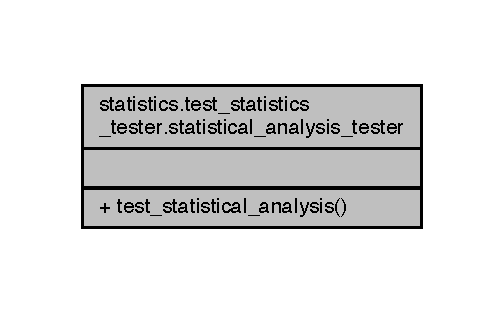
\includegraphics[width=242pt]{d2/d41/classstatistics_1_1test__statistics__tester_1_1statistical__analysis__tester__coll__graph}
\end{center}
\end{figure}
\subsection*{Static Public Member Functions}
\begin{DoxyCompactItemize}
\item 
def \hyperlink{classstatistics_1_1test__statistics__tester_1_1statistical__analysis__tester_ad05a0d6e83aaba083bfba6212ec0b971}{test\+\_\+statistical\+\_\+analysis} ()
\begin{DoxyCompactList}\small\item\em Method to test the methods that support software test automation. \end{DoxyCompactList}\end{DoxyCompactItemize}


\subsection{Detailed Description}


Definition at line \hyperlink{test__statistics__tester_8py_source_l00088}{88} of file \hyperlink{test__statistics__tester_8py_source}{test\+\_\+statistics\+\_\+tester.\+py}.



\subsection{Member Function Documentation}
\hypertarget{classstatistics_1_1test__statistics__tester_1_1statistical__analysis__tester_ad05a0d6e83aaba083bfba6212ec0b971}{}\index{statistics\+::test\+\_\+statistics\+\_\+tester\+::statistical\+\_\+analysis\+\_\+tester@{statistics\+::test\+\_\+statistics\+\_\+tester\+::statistical\+\_\+analysis\+\_\+tester}!test\+\_\+statistical\+\_\+analysis@{test\+\_\+statistical\+\_\+analysis}}
\index{test\+\_\+statistical\+\_\+analysis@{test\+\_\+statistical\+\_\+analysis}!statistics\+::test\+\_\+statistics\+\_\+tester\+::statistical\+\_\+analysis\+\_\+tester@{statistics\+::test\+\_\+statistics\+\_\+tester\+::statistical\+\_\+analysis\+\_\+tester}}
\subsubsection[{test\+\_\+statistical\+\_\+analysis()}]{\setlength{\rightskip}{0pt plus 5cm}def statistics.\+test\+\_\+statistics\+\_\+tester.\+statistical\+\_\+analysis\+\_\+tester.\+test\+\_\+statistical\+\_\+analysis (
\begin{DoxyParamCaption}
{}
\end{DoxyParamCaption}
)\hspace{0.3cm}{\ttfamily [static]}}\label{classstatistics_1_1test__statistics__tester_1_1statistical__analysis__tester_ad05a0d6e83aaba083bfba6212ec0b971}


Method to test the methods that support software test automation. 

\begin{DoxyReturn}{Returns}
-\/ Nothing. O(1) method. 
\end{DoxyReturn}


Definition at line \hyperlink{test__statistics__tester_8py_source_l00095}{95} of file \hyperlink{test__statistics__tester_8py_source}{test\+\_\+statistics\+\_\+tester.\+py}.


\begin{DoxyCode}
\hypertarget{classstatistics_1_1test__statistics__tester_1_1statistical__analysis__tester_l00095}{}\hyperlink{classstatistics_1_1test__statistics__tester_1_1statistical__analysis__tester_ad05a0d6e83aaba083bfba6212ec0b971}{00095}     \textcolor{keyword}{def }\hyperlink{classstatistics_1_1test__statistics__tester_1_1statistical__analysis__tester_ad05a0d6e83aaba083bfba6212ec0b971}{test\_statistical\_analysis}():
00096         print(\textcolor{stringliteral}{"1) Number of test cases passed:  \{\}"} .format(statistical\_analysis.number\_test\_cases\_passed))
00097         print(\textcolor{stringliteral}{"2) Number of test cases used:    \{\}"} .format(statistical\_analysis.number\_test\_cases\_used))
00098         \textcolor{keywordflow}{for} x \textcolor{keywordflow}{in} range(1,7):
00099             statistical\_analysis.increment\_number\_test\_cases\_used()
00100             statistical\_analysis.increment\_number\_test\_cases\_passed()
00101             print(\textcolor{stringliteral}{"Value of x is: \{\}."} .format(x))
00102             print(\textcolor{stringliteral}{"Number of test cases passed: \{\}"} .format(statistical\_analysis.number\_test\_cases\_passed))
00103             print(\textcolor{stringliteral}{"Number of test cases used:   \{\}"} .format(statistical\_analysis.number\_test\_cases\_used))
00104 \end{DoxyCode}


The documentation for this class was generated from the following file\+:\begin{DoxyCompactItemize}
\item 
statistics/\hyperlink{test__statistics__tester_8py}{test\+\_\+statistics\+\_\+tester.\+py}\end{DoxyCompactItemize}

\chapter{File Documentation}
\hypertarget{incremental__test_8py}{}\section{incremental\+\_\+test.\+py File Reference}
\label{incremental__test_8py}\index{incremental\+\_\+test.\+py@{incremental\+\_\+test.\+py}}
\subsection*{Classes}
\begin{DoxyCompactItemize}
\item 
class \hyperlink{classincremental__test_1_1Incremental__Test__Automation}{incremental\+\_\+test.\+Incremental\+\_\+\+Test\+\_\+\+Automation}
\end{DoxyCompactItemize}
\subsection*{Namespaces}
\begin{DoxyCompactItemize}
\item 
 \hyperlink{namespaceincremental__test}{incremental\+\_\+test}
\end{DoxyCompactItemize}
\subsection*{Variables}
\begin{DoxyCompactItemize}
\item 
string \hyperlink{namespaceincremental__test_a5f6427d0e520c9febabce9161afb249b}{incremental\+\_\+test.\+\_\+\+\_\+author\+\_\+\+\_\+} = \textquotesingle{}Zhiyang Ong\textquotesingle{}
\begin{DoxyCompactList}\small\item\em /usr/bin/python /\+Library/\+Frameworks/\+Python.framework/\+Versions/3.\+6/bin/python3 \#!/usr/bin/python -\/mtimeit \end{DoxyCompactList}\item 
string \hyperlink{namespaceincremental__test_a0f94dd1f320b9558e27a5809d2041c4c}{incremental\+\_\+test.\+\_\+\+\_\+version\+\_\+\+\_\+} = \textquotesingle{}1.\+0\textquotesingle{}
\item 
string \hyperlink{namespaceincremental__test_afce713750b4dd215527495dfc84d047e}{incremental\+\_\+test.\+\_\+\+\_\+date\+\_\+\+\_\+} = \textquotesingle{}July 31, 2018\textquotesingle{}
\item 
tuple \hyperlink{namespaceincremental__test_ab5a7aa877c2dae060e3fd03a472cbbf3}{incremental\+\_\+test.\+ip\+\_\+filename} = queue\+\_\+ip\+\_\+args.\+process\+\_\+1st\+\_\+ip\+\_\+arg()
\item 
tuple \hyperlink{namespaceincremental__test_aaf431f9a2a2d1172f09263453438e4f4}{incremental\+\_\+test.\+ip\+\_\+file\+\_\+obj} = file\+\_\+io\+\_\+operations.\+open\+\_\+file\+\_\+object\+\_\+read(ip\+\_\+filename)
\end{DoxyCompactItemize}

\hypertarget{incremental__test_8py_source}{}\section{incremental\+\_\+test.\+py}

\begin{DoxyCode}
\hypertarget{incremental__test_8py_source_l00001}{}\hyperlink{namespaceincremental__test}{00001} \textcolor{comment}{#!/Library/Frameworks/Python.framework/Versions/3.6/bin/python3}
00002 \textcolor{comment}{### /usr/bin/python}
00003 \textcolor{comment}{### /Library/Frameworks/Python.framework/Versions/3.6/bin/python3}
00004 \textcolor{comment}{### #!/usr/bin/python -mtimeit}
00005 
00006 
00007 \textcolor{stringliteral}{"""}
00008 \textcolor{stringliteral}{    This Python script is written by Zhiyang Ong to incrementally}
00009 \textcolor{stringliteral}{        test features for my software solution for genetic technology}
00010 \textcolor{stringliteral}{        mapping.}
00011 \textcolor{stringliteral}{}
00012 \textcolor{stringliteral}{}
00013 \textcolor{stringliteral}{    Synopsis:}
00014 \textcolor{stringliteral}{    Perform incremental software testing automatically for my}
00015 \textcolor{stringliteral}{        genetic technology mapping solution.}
00016 \textcolor{stringliteral}{}
00017 \textcolor{stringliteral}{    This script can be executed as follows:}
00018 \textcolor{stringliteral}{    ./incremental\_test.py [input JSON netlist] [output JSON technology mapping]}
00019 \textcolor{stringliteral}{}
00020 \textcolor{stringliteral}{    Parameters:}
00021 \textcolor{stringliteral}{    [input JSON netlist]:               A JSON file that contains a structural}
00022 \textcolor{stringliteral}{                                            netlist for genetic technology}
00023 \textcolor{stringliteral}{                                            mapping.}
00024 \textcolor{stringliteral}{    [output JSON technology mapping]:   A filename of an output JSON file that}
00025 \textcolor{stringliteral}{                                            contains a genetic technology}
00026 \textcolor{stringliteral}{                                            mapping for the input structural}
00027 \textcolor{stringliteral}{                                            netlist.}
00028 \textcolor{stringliteral}{}
00029 \textcolor{stringliteral}{}
00030 \textcolor{stringliteral}{}
00031 \textcolor{stringliteral}{}
00032 \textcolor{stringliteral}{    Revision History:}
00033 \textcolor{stringliteral}{    July 31, 2018           Version 0.1 Script.}
00034 \textcolor{stringliteral}{"""}
00035 
\hypertarget{incremental__test_8py_source_l00036}{}\hyperlink{namespaceincremental__test_a5f6427d0e520c9febabce9161afb249b}{00036} \_\_author\_\_ = \textcolor{stringliteral}{'Zhiyang Ong'}
\hypertarget{incremental__test_8py_source_l00037}{}\hyperlink{namespaceincremental__test_a0f94dd1f320b9558e27a5809d2041c4c}{00037} \_\_version\_\_ = \textcolor{stringliteral}{'1.0'}
\hypertarget{incremental__test_8py_source_l00038}{}\hyperlink{namespaceincremental__test_afce713750b4dd215527495dfc84d047e}{00038} \_\_date\_\_ = \textcolor{stringliteral}{'July 31, 2018'}
00039 
00040 \textcolor{comment}{#   The MIT License (MIT)}
00041 
00042 \textcolor{comment}{#   Copyright (c) <2018> <Zhiyang Ong>}
00043 
00044 \textcolor{comment}{#   Permission is hereby granted, free of charge, to any person obtaining a copy of this software and
       associated documentation files (the "Software"), to deal in the Software without restriction, including without
       limitation the rights to use, copy, modify, merge, publish, distribute, sublicense, and/or sell copies of the
       Software, and to permit persons to whom the Software is furnished to do so, subject to the following
       conditions:}
00045 
00046 \textcolor{comment}{#   The above copyright notice and this permission notice shall be included in all copies or substantial
       portions of the Software.}
00047 
00048 \textcolor{comment}{#   THE SOFTWARE IS PROVIDED "AS IS", WITHOUT WARRANTY OF ANY KIND, EXPRESS OR IMPLIED, INCLUDING BUT NOT
       LIMITED TO THE WARRANTIES OF MERCHANTABILITY, FITNESS FOR A PARTICULAR PURPOSE AND NONINFRINGEMENT. IN NO
       EVENT SHALL THE AUTHORS OR COPYRIGHT HOLDERS BE LIABLE FOR ANY CLAIM, DAMAGES OR OTHER LIABILITY, WHETHER IN AN
       ACTION OF CONTRACT, TORT OR OTHERWISE, ARISING FROM, OUT OF OR IN CONNECTION WITH THE SOFTWARE OR THE USE
       OR OTHER DEALINGS IN THE SOFTWARE.}
00049 
00050 \textcolor{comment}{#   Email address: echo "cukj -wb- 23wU4X5M589 TROJANS cqkH wiuz2y 0f Mw Stanford" | awk '\{
       sub("23wU4X5M589","F.d\_c\_b. ") sub("Stanford","d0mA1n"); print $5, $2, $8; for (i=1; i<=1; i++) print "6\(\backslash\)b"; print $9, $7,
       $6 \}' | sed y/kqcbuHwM62z/gnotrzadqmC/ | tr 'q' ' ' | tr -d [:cntrl:] | tr -d 'ir' | tr y "\(\backslash\)n"   Che cosa
       significa?}
00051 
00052 
00053 \textcolor{comment}{###############################################################}
00054 \textcolor{stringliteral}{"""}
00055 \textcolor{stringliteral}{    Import modules from The Python Standard Library.}
00056 \textcolor{stringliteral}{    sys         Get access to any command-line arguments.}
00057 \textcolor{stringliteral}{    os          Use any operating system dependent functionality.}
00058 \textcolor{stringliteral}{    os.path     For pathname manipulations.}
00059 \textcolor{stringliteral}{}
00060 \textcolor{stringliteral}{    subprocess -> call}
00061 \textcolor{stringliteral}{                To make system calls.}
00062 \textcolor{stringliteral}{    time        To measure elapsed time.}
00063 \textcolor{stringliteral}{    warnings    Raise warnings.}
00064 \textcolor{stringliteral}{    re          Use regular expressions.}
00065 \textcolor{stringliteral}{}
00066 \textcolor{stringliteral}{    pathlib->Path}
00067 \textcolor{stringliteral}{                For mapping a string to a path.}
00068 \textcolor{stringliteral}{"""}
00069 
00070 \textcolor{keyword}{import} sys
00071 \textcolor{keyword}{import} os
00072 \textcolor{keyword}{import} os.path
00073 \textcolor{comment}{#from pathlib import Path}
00074 \textcolor{keyword}{from} subprocess \textcolor{keyword}{import} call
00075 \textcolor{keyword}{import} time
00076 \textcolor{keyword}{import} warnings
00077 \textcolor{keyword}{import} re
00078 
00079 
00080 
00081 \textcolor{comment}{###############################################################}
00082 \textcolor{comment}{#   Import Custom Python Packages and Modules}
00083 
00084 \textcolor{stringliteral}{"""}
00085 \textcolor{stringliteral}{    Package and module to print statistics of software testing}
00086 \textcolor{stringliteral}{        results.}
00087 \textcolor{stringliteral}{"""}
00088 \textcolor{keyword}{from} \hyperlink{namespacestatistics_1_1test__statistics}{statistics.test\_statistics} \textcolor{keyword}{import} statistical\_analysis
00089 \textcolor{comment}{# Package and module to check the validation of statistical analysis.}
00090 \textcolor{keyword}{from} \hyperlink{namespacestatistics_1_1test__statistics__tester}{statistics.test\_statistics\_tester} \textcolor{keyword}{import} statistical\_analysis\_tester
00091 \textcolor{comment}{# Package and module to process input arguments to the script/program.}
00092 \textcolor{keyword}{from} \hyperlink{namespaceutilities_1_1queue__ip__arguments}{utilities.queue\_ip\_arguments} \textcolor{keyword}{import} queue\_ip\_args
00093 \textcolor{comment}{# Package and module to validate processing of input arguments.}
00094 \textcolor{keyword}{from} \hyperlink{namespaceutilities_1_1queue__ip__arguments__tester}{utilities.queue\_ip\_arguments\_tester} \textcolor{keyword}{import} queue\_ip\_args\_tester
00095 \textcolor{comment}{# Package and module to perform file I/O (input/output) operations.}
00096 \textcolor{keyword}{from} \hyperlink{namespaceutilities_1_1file__io}{utilities.file\_io} \textcolor{keyword}{import} file\_io\_operations
00097 \textcolor{comment}{# Package and module to test file I/O (input/output) operations.}
00098 \textcolor{keyword}{from} \hyperlink{namespaceutilities_1_1file__io__tester}{utilities.file\_io\_tester} \textcolor{keyword}{import} file\_io\_operations\_tester
00099 
00100 \textcolor{comment}{###############################################################}
00101 \textcolor{stringliteral}{"""}
00102 \textcolor{stringliteral}{    Module with methods that incrementally test features for my software}
00103 \textcolor{stringliteral}{        solution for genetic technology mapping.}
00104 \textcolor{stringliteral}{    It tests the following:}
00105 \textcolor{stringliteral}{    + Test the verification code for checking if the input arguments are valid.}
00106 \textcolor{stringliteral}{    + Check if the file I/O module functions correctly.}
00107 \textcolor{stringliteral}{    + Check if the output JSON file generator works correctly.}
00108 \textcolor{stringliteral}{    + Test the implementations for genetic technology mapping.}
00109 \textcolor{stringliteral}{        - Brute force algorithm}
00110 \textcolor{stringliteral}{"""}
\hypertarget{incremental__test_8py_source_l00111}{}\hyperlink{classincremental__test_1_1Incremental__Test__Automation}{00111} \textcolor{keyword}{class }\hyperlink{classincremental__test_1_1Incremental__Test__Automation}{Incremental\_Test\_Automation}:
00112     \textcolor{comment}{# List of BibTeX keys}
\hypertarget{incremental__test_8py_source_l00113}{}\hyperlink{classincremental__test_1_1Incremental__Test__Automation_a8f5272e0488026aa24a829262392f2f7}{00113}     set\_of\_BibTeX\_keys = []
\hypertarget{incremental__test_8py_source_l00114}{}\hyperlink{classincremental__test_1_1Incremental__Test__Automation_ac60587acca9d28d055bd8a7198a987a1}{00114}     num\_of\_bibtex\_entries = 0
00115     \textcolor{comment}{# ============================================================}
00116     \textcolor{comment}{#   Other methods.}
00117     \textcolor{comment}{# ============================================================}
00118     \textcolor{comment}{##  Method to add BibTeX keys into a list, "set\_of\_BibTeX\_keys".}
00119     \textcolor{comment}{#   O(n) method, where n is the number of BibTeX keys.}
00120     @staticmethod
\hypertarget{incremental__test_8py_source_l00121}{}\hyperlink{classincremental__test_1_1Incremental__Test__Automation_a14b316790ae1ef50d84bd4741a4fa020}{00121}     \textcolor{keyword}{def }\hyperlink{classincremental__test_1_1Incremental__Test__Automation_a14b316790ae1ef50d84bd4741a4fa020}{add\_BibTeX\_key}(found\_BibTeX\_key):
00122         \textcolor{keywordflow}{if} (found\_BibTeX\_key \textcolor{keywordflow}{in} Incremental\_Test\_Automation.set\_of\_BibTeX\_keys):
00123             temp\_str = \textcolor{stringliteral}{"Duplicate BibTeX key:"}+found\_BibTeX\_key
00124             warnings.warn(temp\_str)
00125             \textcolor{keywordflow}{raise} Exception(\textcolor{stringliteral}{"Multiple instances of a BibTeX key"})
00126         Incremental\_Test\_Automation.set\_of\_BibTeX\_keys.append(found\_BibTeX\_key)
00127     \textcolor{comment}{# ============================================================}
00128     \textcolor{comment}{##  Method to sort BibTeX keys into a list, "set\_of\_BibTeX\_keys".}
00129     \textcolor{comment}{#   O(n*log(n)) method, where n is the number of BibTeX keys.}
00130     @staticmethod
\hypertarget{incremental__test_8py_source_l00131}{}\hyperlink{classincremental__test_1_1Incremental__Test__Automation_a856c60714b5d716d5eb630cbc3d55d09}{00131}     \textcolor{keyword}{def }\hyperlink{classincremental__test_1_1Incremental__Test__Automation_a856c60714b5d716d5eb630cbc3d55d09}{sort\_BibTeX\_keys}():
00132         Incremental\_Test\_Automation.set\_of\_BibTeX\_keys = sorted(
      Incremental\_Test\_Automation.set\_of\_BibTeX\_keys)
00133     \textcolor{comment}{# ============================================================}
00134     \textcolor{comment}{##  Method to read each line of the input BibTeX file.}
00135     \textcolor{comment}{#   O(n) method, where n is the number of lines of the BibTeX file.}
00136     @staticmethod
\hypertarget{incremental__test_8py_source_l00137}{}\hyperlink{classincremental__test_1_1Incremental__Test__Automation_a7cec6a541c4680c857a699dbe363ffbd}{00137}     \textcolor{keyword}{def }\hyperlink{classincremental__test_1_1Incremental__Test__Automation_a7cec6a541c4680c857a699dbe363ffbd}{read\_input\_BibTeX\_file}(ip\_file\_object,input\_BibTeX\_file):
00138         \textcolor{comment}{#print "--------------------------------------------------------"}
00139         println = \textcolor{stringliteral}{"=    Reading input BibTeX file: "}
00140         println += input\_BibTeX\_file
00141         print(println)
00142         \textcolor{comment}{# Read each available line in the input BibTeX file.}
00143         \textcolor{keywordflow}{for} line \textcolor{keywordflow}{in} ip\_file\_object:
00144             \textcolor{comment}{# Is this line the 1st line of a BibTeX entry?}
00145             \textcolor{keywordflow}{if} \textcolor{stringliteral}{"@"} == line[0]:
00146                 \textcolor{comment}{# Yes.}
00147 \textcolor{comment}{#               print "...  First line of a BibTeX entry."}
00148                 \textcolor{comment}{# Increment number of BibTeX entries.}
00149                 Incremental\_Test\_Automation.num\_of\_bibtex\_entries = 
      Incremental\_Test\_Automation.num\_of\_bibtex\_entries + 1
00150                 tokenized\_BibTeX\_entry = re.split(\textcolor{stringliteral}{'@|\{|,'},line)
00151 \textcolor{comment}{#               for i in tokenized\_BibTeX\_entry:}
00152 \textcolor{comment}{#                   print i}
00153                 \textcolor{comment}{# Is the type of the BibTeX entry valid?}
00154                 \textcolor{keywordflow}{if} (tokenized\_BibTeX\_entry[1] \textcolor{keywordflow}{in} queue\_ip\_args.BibTeX\_entry\_types):
00155                     \textcolor{comment}{# Yes. Try adding the BibTeX entry to "set\_of\_BibTeX\_keys".}
00156                     Incremental\_Test\_Automation.add\_BibTeX\_key(tokenized\_BibTeX\_entry[2].lower())
00157                 \textcolor{keywordflow}{else}:
00158                     \textcolor{comment}{# No. Warn user that the type of BibTeX entry is invalid!}
00159                     temp\_str = \textcolor{stringliteral}{"Invalid type of BibTeX entry:"}
00160                     temp\_str += tokenized\_BibTeX\_entry[1]
00161                     print(temp\_str)
00162                     \textcolor{comment}{#warnings.warn("Invalid type of BibTeX entry")}
00163                     \textcolor{keywordflow}{raise} Exception(\textcolor{stringliteral}{"BibTeX entry has an invalid type!"})
00164         \textcolor{keywordflow}{if} (Incremental\_Test\_Automation.num\_of\_bibtex\_entries != len(
      Incremental\_Test\_Automation.set\_of\_BibTeX\_keys)):
00165             \textcolor{keywordflow}{raise} Exception(\textcolor{stringliteral}{"Mismatch in number of BibTeX entries processed."})
00166         \textcolor{keywordflow}{else}:
00167             print(\textcolor{stringliteral}{"=    Number of BibTeX entries processed: \{\}"} .format(str(
      Incremental\_Test\_Automation.num\_of\_bibtex\_entries)))
00168 
00169 
00170 
00171 
00172 
00173 
00174 
00175 
00176 
00177 
00178 
00179 \textcolor{comment}{###############################################################}
00180 \textcolor{comment}{# Main method for the program.}
00181 
00182 \textcolor{comment}{#   If this is executed as a Python script,}
00183 \textcolor{keywordflow}{if} \_\_name\_\_ == \textcolor{stringliteral}{"\_\_main\_\_"}:
00184     print(\textcolor{stringliteral}{"=================================================="})
00185     print(\textcolor{stringliteral}{"Automating incremental regression testing of my software"})
00186     print(\textcolor{stringliteral}{" solution for genetic technology mapping."})
00187     print(\textcolor{stringliteral}{""})
00188     \textcolor{comment}{# Assign input arguments to "queue\_ip\_args" for processing.}
00189     \textcolor{comment}{#queue\_ip\_args.set\_input\_arguments(sys.argv,queue\_ip\_args.INCREMENTAL\_TEST)}
00190     queue\_ip\_args.set\_input\_arguments(sys.argv)
00191     \textcolor{comment}{# Check if user wants to read the brief user manual.}
00192     queue\_ip\_args.check\_if\_help\_wanted()
00193     \textcolor{comment}{# Process the first input argument.}
00194     print(\textcolor{stringliteral}{"=    Process the first input argument."})
\hypertarget{incremental__test_8py_source_l00195}{}\hyperlink{namespaceincremental__test_ab5a7aa877c2dae060e3fd03a472cbbf3}{00195}     ip\_filename = queue\_ip\_args.process\_1st\_ip\_arg()
00196     \textcolor{comment}{# Create a file object for reading.}
00197     print(\textcolor{stringliteral}{"=    Create a file object for reading."})
00198     \textcolor{comment}{# Create a file object for input BibTeX file, in reading mode.}
\hypertarget{incremental__test_8py_source_l00199}{}\hyperlink{namespaceincremental__test_aaf431f9a2a2d1172f09263453438e4f4}{00199}     ip\_file\_obj = file\_io\_operations.open\_file\_object\_read(ip\_filename)
00200     \textcolor{comment}{# The real stuff begins here...}
00201     statistical\_analysis\_tester.test\_statistical\_analysis()
00202     \textcolor{comment}{#   ### TO-DO}
00203     \textcolor{comment}{# Insert test cases for testing the utilities package.}
00204     print(\textcolor{stringliteral}{"-    -   -   -   -   -   -   -   -   -   -   -   -"})
00205 \textcolor{comment}{#   check\_bibtex\_key\_tester.test\_check\_bibtex\_key()}
00206     queue\_ip\_args\_tester.test\_queue\_ip\_args()
00207     print(\textcolor{stringliteral}{"-    -   -   -   -   -   -   -   -   -   -   -   -"})
00208     file\_io\_operations\_tester.test\_queue\_ip\_args()
00209     print(\textcolor{stringliteral}{"-    -   -   -   -   -   -   -   -   -   -   -   -"})
00210 \textcolor{comment}{#   Incremental\_Test\_Automation.read\_input\_BibTeX\_file(ip\_file\_obj,ip\_filename)}
00211     print(\textcolor{stringliteral}{"!    !   !   !   !   !   !   !   !   !   !"})
00212     print(\textcolor{stringliteral}{">>   Get statistics of the software testing process."})
00213     statistical\_analysis.print\_statistics\_of\_software\_testing()
00214     \textcolor{comment}{# Close the file object for reading.}
00215     print(\textcolor{stringliteral}{"=    Close the file object for reading."})
00216     file\_io\_operations.close\_file\_object(ip\_file\_obj)
\end{DoxyCode}

\hypertarget{README_8md}{}\section{R\+E\+A\+D\+M\+E.\+md File Reference}
\label{README_8md}\index{R\+E\+A\+D\+M\+E.\+md@{R\+E\+A\+D\+M\+E.\+md}}

\hypertarget{README_8md_source}{}\section{R\+E\+A\+D\+M\+E.\+md}

\begin{DoxyCode}
00001 # 2018-wannabe-postdoc-1
00002 
00003 This is the repository for problem 1 of the 2018 BDAthlon programming contest.
00004 
00005 It my solution for the problem on genetic technology mapping.
00006 
00007 
00008 ## Organization of the Repository
00009 
00010 + docs
00011    - Documentation generated by documentation generators
00012        * Doxygen
00013        * pydoc (for Python scripts): /usr/bin/pydoc
00014 + notes
00015    - Software licenses
00016        * *MIT License*.
00017    - Guidelines for collaborating on open source software and/or hardware
00018       projects.
00019     * Documentation about guidelines that I am following for my research,
00020          and for my research collaborators to know about.
00021   - Externalities list.
00022     * *Publicly available library, API, or framework* that I have used as
00023         external components for my software.
00024        * Some *Python* modules from the repository
       [bibtex-analytics](https://github.com/eda-ricercatore/bibtex-analytics),
00025            which I developed.
00026 
00027 
00028 ##  Description of the Software Solution for Genetic Technology Mapping
00029 
00030 My solution for genetic technology mapping, **problem1\_solution.py**, takes in
00031    two input parameters, **[input JSON netlist]** and **[output JSON technology mapping]**.
00032 
00033 The first input parameter **[input JSON netlist]** is a JSON file that contains
00034    a structural netlist for genetic technology mapping.
00035 
00036 The other input parameter **[output JSON technology mapping]** is the filename
00037    of an output JSON file that contains a genetic technology mapping for the
00038    input structural netlist (**[input JSON netlist]**).
00039 
00040 The front-end of **problem1\_solution.py** parses the input arguments, checks
00041    their validity, and parses the input structural netlist for genetic
00042    technology mapping.
00043 
00044 The genetic technology mapping engine of **problem1\_solution.py** consists of a
00045    (set of) solution(s) to perform genetic technology mapping.
00046    A solution is an implementation of a known/new algorithm/heuristic for
00047        genetic technology mapping.
00048 
00049 Solution *1a* performs *brute force search* to explore different options for
00050    genetic technology mapping.
00051 
00052 
00053 The back-end of **problem1\_solution.py** generates an output file containing
00054    the genetic technology mapping of the input genetic circuit, in JSON format.
00055 
00056 
00057 
00058 
00059 
00060 
00061 
00062 
00063 ##  Instructions on How to Build and Run the Software Solution
00064 
00065 ###    Building and Executing the Software Solution
00066 
00067 To execute the software solution, try:
00068 
00069    ./problem1\_solution.py [input JSON netlist] [output JSON technology mapping]
00070 
00071 Input Parameters:
00072 [input JSON netlist]:                          A JSON file that contains a structural
00073                                                                        netlist for genetic technology
       mapping.
00074 
00075 [output JSON technology mapping]:  A filename of an output JSON file that
00076                                                                        contains a genetic technology
       mapping for
00077                                                                        the input structural netlist.
00078 
00079 
00080 ###    Documentation Generation
00081 
00082 To use *Doxygen* to generate documentation for the Python software, try:
00083 
00084    make doxygen
00085 
00086 To view the *Doxygen*-generated documention, open the file
       [**docs/html/index.html**](https://github.com/BDAthlon/2018-wannabe-postdoc-1/blob/master/docs/html/index.html) in a Web browser.
00087 
00088 The command **make doxygeninit** has already been used to generate a *Doxygen*
00089    configuration file named **doxygen.config**.
00090    **DO NOT RUN THE COMMAND *doxygen.config* AGAIN!!!**
00091 
00092 To use *pydoc* to view or generate documentation for my software solution
00093    (Python code), try:
00094 
00095    pydoc [*Python* package/module/class]
00096 
00097 A *Python* package corresponds to a subdirectory of this repository, while a
00098    *Python* module/class corresponds to a *Python* source file in a subdirectory.
00099 
00100 
00101 
00102 #  References
00103 
00104 Citations/References that use the LaTeX/BibTeX notation are taken from my
00105    BibTeX database (set of BibTeX entries).
00106 
00107 Additional references not found in the reference list shall be indicated below (TO BE UPDATED).
00108 
00109 
00110    @misc\{Roehner2018,
00111        Address = \{Boston, \{MA\}\},
00112        Author = \{Nicholas Roehner and Curtis Madsen\},
00113        Howpublished = \{Self-published\},
00114        Month = \{July 31\},
00115        Publisher = \{Boston University\},
00116        School = \{Boston University\},
00117        Title = \{BDAthlon 2018\},
00118        Year = \{2018\}\}
00119 
00120 
00121 
00122 #  Author Information
00123 
00124 The MIT License (MIT)
00125 
00126 Copyright (c) <2018> Zhiyang Ong
00127 
00128 Permission is hereby granted, free of charge, to any person obtaining a copy of this software and
       associated documentation files (the "Software"), to deal in the Software without restriction, including without
       limitation the rights to use, copy, modify, merge, publish, distribute, sublicense, and/or sell copies of
       the Software, and to permit persons to whom the Software is furnished to do so, subject to the following
       conditions:
00129 
00130 The above copyright notice and this permission notice shall be included in all copies or substantial
       portions of the Software.
00131 
00132 THE SOFTWARE IS PROVIDED "AS IS", WITHOUT WARRANTY OF ANY KIND, EXPRESS OR IMPLIED, INCLUDING BUT NOT
       LIMITED TO THE WARRANTIES OF MERCHANTABILITY, FITNESS FOR A PARTICULAR PURPOSE AND NONINFRINGEMENT. IN NO
       EVENT SHALL THE AUTHORS OR COPYRIGHT HOLDERS BE LIABLE FOR ANY CLAIM, DAMAGES OR OTHER LIABILITY, WHETHER IN
       AN ACTION OF CONTRACT, TORT OR OTHERWISE, ARISING FROM, OUT OF OR IN CONNECTION WITH THE SOFTWARE OR THE USE
       OR OTHER DEALINGS IN THE SOFTWARE.
00133 
00134 Email address: echo "cukj -wb- 23wU4X5M589 TROJANS cqkH wiuz2y 0f Mw Stanford" | awk '\{
       sub("23wU4X5M589","F.d\_c\_b. ") sub("Stanford","d0mA1n"); print $5, $2, $8; for (i=1; i<=1; i++) print "6\(\backslash\)b"; print $9, $7,
       $6 \}' | sed y/kqcbuHwM62z/gnotrzadqmC/ | tr 'q' ' ' | tr -d [:cntrl:] | tr -d 'ir' | tr y "\(\backslash\)n"      Don't
       compromise my computing accounts. You have been warned.
\end{DoxyCode}

\hypertarget{statistics_2____init_____8py}{}\section{statistics/\+\_\+\+\_\+init\+\_\+\+\_\+.py File Reference}
\label{statistics_2____init_____8py}\index{statistics/\+\_\+\+\_\+init\+\_\+\+\_\+.\+py@{statistics/\+\_\+\+\_\+init\+\_\+\+\_\+.\+py}}
\subsection*{Namespaces}
\begin{DoxyCompactItemize}
\item 
 \hyperlink{namespacestatistics}{statistics}
\end{DoxyCompactItemize}

\hypertarget{statistics_2____init_____8py_source}{}\section{\+\_\+\+\_\+init\+\_\+\+\_\+.\+py}
\label{statistics_2____init_____8py_source}\index{statistics/\+\_\+\+\_\+init\+\_\+\+\_\+.\+py@{statistics/\+\_\+\+\_\+init\+\_\+\+\_\+.\+py}}

\begin{DoxyCode}
\end{DoxyCode}

\hypertarget{utilities_2____init_____8py}{}\section{utilities/\+\_\+\+\_\+init\+\_\+\+\_\+.py File Reference}
\label{utilities_2____init_____8py}\index{utilities/\+\_\+\+\_\+init\+\_\+\+\_\+.\+py@{utilities/\+\_\+\+\_\+init\+\_\+\+\_\+.\+py}}
\subsection*{Namespaces}
\begin{DoxyCompactItemize}
\item 
 \hyperlink{namespaceutilities}{utilities}
\end{DoxyCompactItemize}

\hypertarget{utilities_2____init_____8py_source}{}\section{\+\_\+\+\_\+init\+\_\+\+\_\+.\+py}
\label{utilities_2____init_____8py_source}\index{utilities/\+\_\+\+\_\+init\+\_\+\+\_\+.\+py@{utilities/\+\_\+\+\_\+init\+\_\+\+\_\+.\+py}}

\begin{DoxyCode}
\end{DoxyCode}

\hypertarget{test__statistics_8py}{}\section{statistics/test\+\_\+statistics.py File Reference}
\label{test__statistics_8py}\index{statistics/test\+\_\+statistics.\+py@{statistics/test\+\_\+statistics.\+py}}
\subsection*{Classes}
\begin{DoxyCompactItemize}
\item 
class \hyperlink{classstatistics_1_1test__statistics_1_1statistical__analysis}{statistics.\+test\+\_\+statistics.\+statistical\+\_\+analysis}
\begin{DoxyCompactList}\small\item\em Import Custom Python Modules. \end{DoxyCompactList}\end{DoxyCompactItemize}
\subsection*{Namespaces}
\begin{DoxyCompactItemize}
\item 
 \hyperlink{namespacestatistics_1_1test__statistics}{statistics.\+test\+\_\+statistics}
\end{DoxyCompactItemize}
\subsection*{Variables}
\begin{DoxyCompactItemize}
\item 
string \hyperlink{namespacestatistics_1_1test__statistics_a188ace18635f13c413bf14347b4eb7f0}{statistics.\+test\+\_\+statistics.\+\_\+\+\_\+author\+\_\+\+\_\+} = \textquotesingle{}Zhiyang Ong\textquotesingle{}
\begin{DoxyCompactList}\small\item\em /usr/bin/python /\+Library/\+Frameworks/\+Python.framework/\+Versions/3.\+6/bin/python3 \end{DoxyCompactList}\item 
string \hyperlink{namespacestatistics_1_1test__statistics_ad5c236202b813efcbc877e38a20d7f07}{statistics.\+test\+\_\+statistics.\+\_\+\+\_\+version\+\_\+\+\_\+} = \textquotesingle{}1.\+0\textquotesingle{}
\item 
string \hyperlink{namespacestatistics_1_1test__statistics_a271285b175d250f7888c9b41fa124abd}{statistics.\+test\+\_\+statistics.\+\_\+\+\_\+date\+\_\+\+\_\+} = \textquotesingle{}December 15, 2017\textquotesingle{}
\end{DoxyCompactItemize}

\hypertarget{test__statistics_8py_source}{}\section{test\+\_\+statistics.\+py}
\label{test__statistics_8py_source}\index{statistics/test\+\_\+statistics.\+py@{statistics/test\+\_\+statistics.\+py}}

\begin{DoxyCode}
\hypertarget{test__statistics_8py_source_l00001}{}\hyperlink{namespacestatistics_1_1test__statistics}{00001} \textcolor{comment}{#!/Library/Frameworks/Python.framework/Versions/3.6/bin/python3}
00002 \textcolor{comment}{### /usr/bin/python}
00003 \textcolor{comment}{### /Library/Frameworks/Python.framework/Versions/3.6/bin/python3}
00004 
00005 
00006 \textcolor{stringliteral}{"""}
00007 \textcolor{stringliteral}{    This Python script is written by Zhiyang Ong to perform}
00008 \textcolor{stringliteral}{        operations to support basic statistical analysis}
00009 \textcolor{stringliteral}{        during software test automation.}
00010 \textcolor{stringliteral}{}
00011 \textcolor{stringliteral}{}
00012 \textcolor{stringliteral}{    Synopsis:}
00013 \textcolor{stringliteral}{    Perform statistical analysis during software test}
00014 \textcolor{stringliteral}{        automation.}
00015 \textcolor{stringliteral}{}
00016 \textcolor{stringliteral}{}
00017 \textcolor{stringliteral}{    Revision History:}
00018 \textcolor{stringliteral}{    December 15, 2017           Version 0.1, initial build.}
00019 \textcolor{stringliteral}{"""}
00020 
\hypertarget{test__statistics_8py_source_l00021}{}\hyperlink{namespacestatistics_1_1test__statistics_a188ace18635f13c413bf14347b4eb7f0}{00021} \_\_author\_\_ = \textcolor{stringliteral}{'Zhiyang Ong'}
\hypertarget{test__statistics_8py_source_l00022}{}\hyperlink{namespacestatistics_1_1test__statistics_ad5c236202b813efcbc877e38a20d7f07}{00022} \_\_version\_\_ = \textcolor{stringliteral}{'1.0'}
\hypertarget{test__statistics_8py_source_l00023}{}\hyperlink{namespacestatistics_1_1test__statistics_a271285b175d250f7888c9b41fa124abd}{00023} \_\_date\_\_ = \textcolor{stringliteral}{'December 15, 2017'}
00024 
00025 \textcolor{comment}{#   The MIT License (MIT)}
00026 
00027 \textcolor{comment}{#   Copyright (c) <2014-2018> <Zhiyang Ong>}
00028 
00029 \textcolor{comment}{#   Permission is hereby granted, free of charge, to any person obtaining a copy of this software and
       associated documentation files (the "Software"), to deal in the Software without restriction, including without
       limitation the rights to use, copy, modify, merge, publish, distribute, sublicense, and/or sell copies of the
       Software, and to permit persons to whom the Software is furnished to do so, subject to the following
       conditions:}
00030 
00031 \textcolor{comment}{#   The above copyright notice and this permission notice shall be included in all copies or substantial
       portions of the Software.}
00032 
00033 \textcolor{comment}{#   THE SOFTWARE IS PROVIDED "AS IS", WITHOUT WARRANTY OF ANY KIND, EXPRESS OR IMPLIED, INCLUDING BUT NOT
       LIMITED TO THE WARRANTIES OF MERCHANTABILITY, FITNESS FOR A PARTICULAR PURPOSE AND NONINFRINGEMENT. IN NO
       EVENT SHALL THE AUTHORS OR COPYRIGHT HOLDERS BE LIABLE FOR ANY CLAIM, DAMAGES OR OTHER LIABILITY, WHETHER IN AN
       ACTION OF CONTRACT, TORT OR OTHERWISE, ARISING FROM, OUT OF OR IN CONNECTION WITH THE SOFTWARE OR THE USE
       OR OTHER DEALINGS IN THE SOFTWARE.}
00034 
00035 \textcolor{comment}{#   Email address: echo "cukj -wb- 23wU4X5M589 TROJANS cqkH wiuz2y 0f Mw Stanford" | awk '\{
       sub("23wU4X5M589","F.d\_c\_b. ") sub("Stanford","d0mA1n"); print $5, $2, $8; for (i=1; i<=1; i++) print "6\(\backslash\)b"; print $9, $7,
       $6 \}' | sed y/kqcbuHwM62z/gnotrzadqmC/ | tr 'q' ' ' | tr -d [:cntrl:] | tr -d 'ir' | tr y "\(\backslash\)n"   Che cosa
       significa?}
00036 
00037 \textcolor{comment}{###############################################################}
00038 \textcolor{stringliteral}{"""}
00039 \textcolor{stringliteral}{    Import modules from The Python Standard Library.}
00040 \textcolor{stringliteral}{    sys         Get access to any command-line arguments.}
00041 \textcolor{stringliteral}{    os          Use any operating system dependent functionality.}
00042 \textcolor{stringliteral}{    os.path     For pathname manipulations.}
00043 \textcolor{stringliteral}{}
00044 \textcolor{stringliteral}{    subprocess -> call}
00045 \textcolor{stringliteral}{                To make system calls.}
00046 \textcolor{stringliteral}{}
00047 \textcolor{stringliteral}{    time        To measure elapsed time.}
00048 \textcolor{stringliteral}{    warnings    Raise warnings.}
00049 \textcolor{stringliteral}{    re          Use regular expressions.}
00050 \textcolor{stringliteral}{}
00051 \textcolor{stringliteral}{    collections -> namedtuple}
00052 \textcolor{stringliteral}{                To use named tuples.}
00053 \textcolor{stringliteral}{    operator -> attrgetter}
00054 \textcolor{stringliteral}{                To manipulate attributes of a named tuple as callable}
00055 \textcolor{stringliteral}{                    objects.}
00056 \textcolor{stringliteral}{"""}
00057 
00058 \textcolor{comment}{#import sys}
00059 \textcolor{comment}{#import os}
00060 \textcolor{comment}{#import os.path}
00061 \textcolor{comment}{#from subprocess import call}
00062 \textcolor{comment}{#import time}
00063 \textcolor{keyword}{import} warnings
00064 \textcolor{comment}{#import re}
00065 \textcolor{comment}{#from collections import namedtuple}
00066 \textcolor{comment}{#from operator import attrgetter}
00067 
00068 \textcolor{comment}{###############################################################}
00069 \textcolor{comment}{#   Import Custom Python Modules}
00070 
00071 
00072 
00073 
00074 
00075 
00076 \textcolor{comment}{###############################################################}
00077 \textcolor{stringliteral}{"""}
00078 \textcolor{stringliteral}{    Module with methods that perform basic statistical analysis}
00079 \textcolor{stringliteral}{        during software test automation.}
00080 \textcolor{stringliteral}{"""}
\hypertarget{test__statistics_8py_source_l00081}{}\hyperlink{classstatistics_1_1test__statistics_1_1statistical__analysis}{00081} \textcolor{keyword}{class }\hyperlink{classstatistics_1_1test__statistics_1_1statistical__analysis}{statistical\_analysis}:
00082     \textcolor{comment}{#   Variable declaration.}
00083     \textcolor{comment}{#}
00084     \textcolor{comment}{#   Number of test cases used.}
\hypertarget{test__statistics_8py_source_l00085}{}\hyperlink{classstatistics_1_1test__statistics_1_1statistical__analysis_afed7a27a010e7377d2719b315d5d5f17}{00085}     number\_test\_cases\_used = 0
00086     \textcolor{comment}{#   Number of test cases passed.}
\hypertarget{test__statistics_8py_source_l00087}{}\hyperlink{classstatistics_1_1test__statistics_1_1statistical__analysis_ac7555db570919cec38a8325d8427093e}{00087}     number\_test\_cases\_passed = 0
00088     \textcolor{comment}{# =========================================================}
00089     \textcolor{comment}{#   Accessor methods.}
00090     \textcolor{comment}{# =========================================================}
00091     \textcolor{comment}{#   Method to access the number of test cases used.}
00092     \textcolor{comment}{#   @return - Nothing.}
00093     \textcolor{comment}{#   @postcondition - number\_test\_cases\_used < number\_test\_cases\_passed.}
00094     \textcolor{comment}{#   O(1) method.}
00095     @staticmethod
\hypertarget{test__statistics_8py_source_l00096}{}\hyperlink{classstatistics_1_1test__statistics_1_1statistical__analysis_a8bddd92400d64e68caf934defa5ededb}{00096}     \textcolor{keyword}{def }\hyperlink{classstatistics_1_1test__statistics_1_1statistical__analysis_a8bddd92400d64e68caf934defa5ededb}{get\_number\_test\_cases\_used}():
00097         \textcolor{keywordflow}{return} statistical\_analysis.number\_test\_cases\_used
00098     \textcolor{comment}{# =========================================================}
00099     \textcolor{comment}{#   Method to access the number of test cases passed.}
00100     \textcolor{comment}{#   @return - Nothing.}
00101     \textcolor{comment}{#   @postcondition - number\_test\_cases\_used < number\_test\_cases\_passed.}
00102     \textcolor{comment}{#   O(1) method.}
00103     @staticmethod
\hypertarget{test__statistics_8py_source_l00104}{}\hyperlink{classstatistics_1_1test__statistics_1_1statistical__analysis_a0461b276e37fd6c24ab919efbeb04309}{00104}     \textcolor{keyword}{def }\hyperlink{classstatistics_1_1test__statistics_1_1statistical__analysis_a0461b276e37fd6c24ab919efbeb04309}{get\_number\_test\_cases\_passed}():
00105         \textcolor{keywordflow}{return} statistical\_analysis.number\_test\_cases\_passed
00106     \textcolor{comment}{# =========================================================}
00107     \textcolor{comment}{#   Mutator methods.}
00108     \textcolor{comment}{# =========================================================}
00109     \textcolor{comment}{#   Method to increment the number of test cases used.}
00110     \textcolor{comment}{#   @return - Nothing.}
00111     \textcolor{comment}{#   @postcondition - number\_test\_cases\_used < number\_test\_cases\_passed.}
00112     \textcolor{comment}{#   O(1) method.}
00113     @staticmethod
\hypertarget{test__statistics_8py_source_l00114}{}\hyperlink{classstatistics_1_1test__statistics_1_1statistical__analysis_a7e88e87c8e6739dcaa37740985089f11}{00114}     \textcolor{keyword}{def }\hyperlink{classstatistics_1_1test__statistics_1_1statistical__analysis_a7e88e87c8e6739dcaa37740985089f11}{increment\_number\_test\_cases\_used}():
00115         \textcolor{keywordflow}{if} 0 == statistical\_analysis.number\_test\_cases\_used:
00116             statistical\_analysis.number\_test\_cases\_used = 1
00117         \textcolor{keywordflow}{else}:
00118             statistical\_analysis.number\_test\_cases\_used = statistical\_analysis.number\_test\_cases\_used + 1
00119         \textcolor{keywordflow}{if} (statistical\_analysis.number\_test\_cases\_used < statistical\_analysis.number\_test\_cases\_passed):
00120             print(\textcolor{stringliteral}{" Problem: number\_test\_cases\_used < number\_test\_cases\_passed"})
00121             \textcolor{keywordflow}{raise} Exception(\textcolor{stringliteral}{"   Error in incrementing number\_test\_cases\_used"})
00122     \textcolor{comment}{# =========================================================}
00123     \textcolor{comment}{#   Method to increment the number of test cases passed.}
00124     \textcolor{comment}{#   @return - Nothing.}
00125     \textcolor{comment}{#   @postcondition - number\_test\_cases\_used < number\_test\_cases\_passed.}
00126     \textcolor{comment}{#   O(1) method.}
00127     @staticmethod
\hypertarget{test__statistics_8py_source_l00128}{}\hyperlink{classstatistics_1_1test__statistics_1_1statistical__analysis_a056f55c0e7f60e29d4b37e8e74d3cd08}{00128}     \textcolor{keyword}{def }\hyperlink{classstatistics_1_1test__statistics_1_1statistical__analysis_a056f55c0e7f60e29d4b37e8e74d3cd08}{increment\_number\_test\_cases\_passed}():
00129         \textcolor{keywordflow}{if} 0 == statistical\_analysis.number\_test\_cases\_passed:
00130             statistical\_analysis.number\_test\_cases\_passed = 1
00131         \textcolor{keywordflow}{else}:
00132             statistical\_analysis.number\_test\_cases\_passed = statistical\_analysis.number\_test\_cases\_passed +
       1
00133         \textcolor{keywordflow}{if} (statistical\_analysis.number\_test\_cases\_used < statistical\_analysis.number\_test\_cases\_passed):
00134             print(\textcolor{stringliteral}{"Number of test cases passed: \{\}"} .format(statistical\_analysis.number\_test\_cases\_passed))
00135             print(\textcolor{stringliteral}{"Number of test cases used:   \{\}"} .format(statistical\_analysis.number\_test\_cases\_used))
00136             print(\textcolor{stringliteral}{" Problem: number\_test\_cases\_used < number\_test\_cases\_passed"})
00137             \textcolor{keywordflow}{raise} Exception(\textcolor{stringliteral}{"   Error with number\_test\_cases\_used."})
00138     \textcolor{comment}{# =========================================================}
00139     \textcolor{comment}{#   Other methods.}
00140     \textcolor{comment}{# =========================================================}
00141     \textcolor{comment}{#   Method to determine percentage of test cases passed.}
00142     \textcolor{comment}{#   @return - percentage of test cases passed.}
00143     \textcolor{comment}{#   @precondition - number\_test\_cases\_used < number\_test\_cases\_passed.}
00144     \textcolor{comment}{#   O(1) method.}
00145     @staticmethod
\hypertarget{test__statistics_8py_source_l00146}{}\hyperlink{classstatistics_1_1test__statistics_1_1statistical__analysis_a1bec04d2404b2bdf277c4ba170abb4a1}{00146}     \textcolor{keyword}{def }\hyperlink{classstatistics_1_1test__statistics_1_1statistical__analysis_a1bec04d2404b2bdf277c4ba170abb4a1}{get\_test\_cases\_passed\_average}():
00147         \textcolor{keywordflow}{if} (statistical\_analysis.number\_test\_cases\_used > statistical\_analysis.number\_test\_cases\_passed):
00148             print(\textcolor{stringliteral}{" Problem: number\_test\_cases\_used > number\_test\_cases\_passed"})
00149             \textcolor{keywordflow}{raise} Exception(\textcolor{stringliteral}{"   Precondition failed (1): see number\_test\_cases\_used or
       number\_test\_cases\_passed."})
00150         \textcolor{keywordflow}{return} (statistical\_analysis.number\_test\_cases\_passed*100 / 
      statistical\_analysis.number\_test\_cases\_used)
00151     \textcolor{comment}{# =========================================================}
00152     \textcolor{comment}{#   Method to print statistics of software testing results.}
00153     \textcolor{comment}{#   @return - Nothing}
00154     \textcolor{comment}{#   @precondition - number\_test\_cases\_used < number\_test\_cases\_passed.}
00155     \textcolor{comment}{#   O(1) method.}
00156     @staticmethod
\hypertarget{test__statistics_8py_source_l00157}{}\hyperlink{classstatistics_1_1test__statistics_1_1statistical__analysis_ad6bdf2cde8553974d93d5971870970d8}{00157}     \textcolor{keyword}{def }\hyperlink{classstatistics_1_1test__statistics_1_1statistical__analysis_ad6bdf2cde8553974d93d5971870970d8}{print\_statistics\_of\_software\_testing}():
00158         \textcolor{keywordflow}{if} (statistical\_analysis.number\_test\_cases\_used < statistical\_analysis.number\_test\_cases\_passed):
00159             print(\textcolor{stringliteral}{" Problem: number\_test\_cases\_used < number\_test\_cases\_passed"})
00160             \textcolor{keywordflow}{raise} Exception(\textcolor{stringliteral}{"   Precondition failed (2): see number\_test\_cases\_used or
       number\_test\_cases\_passed."})
00161         print(\textcolor{stringliteral}{"*    Number of test cases passed:        \{\}"} .format(
      statistical\_analysis.number\_test\_cases\_passed))
00162         print(\textcolor{stringliteral}{"*    Number of test cases used:      \{\}"} .format(statistical\_analysis.number\_test\_cases\_used
      ))
00163         print(\textcolor{stringliteral}{"*    Percentage of test cases passed:    \{\}%."} .format((
      statistical\_analysis.number\_test\_cases\_passed*100/statistical\_analysis.number\_test\_cases\_used)))
00164         \textcolor{comment}{#print "*   Percentage of test cases passed:    
      ",statistical\_analysis.get\_test\_cases\_passed\_average(),"%."}
00165         \textcolor{comment}{#   Format printing of the statistics as follows.}
00166         \textcolor{comment}{#print "*   Percentage of test cases passed:    ",(13*100/19),"%."}
00167         \textcolor{comment}{#   Most of the following cannot calculate the percentage properly.}
00168         \textcolor{comment}{#print "*   Percentage of test cases passed:    ",(13/19)*100,"%."}
00169         \textcolor{comment}{#print "*   Percentage of test cases passed:    ",(13/19)*(10000/100),"%."}
00170         \textcolor{comment}{#print "*   Percentage of test cases passed:    ",(10000/100)*(13/19),"%."}
00171         \textcolor{comment}{#print "*   Percentage of test cases passed:    ",(13*10000)/(19*100),"%."}
\end{DoxyCode}

\hypertarget{test__statistics__tester_8py}{}\section{statistics/test\+\_\+statistics\+\_\+tester.py File Reference}
\label{test__statistics__tester_8py}\index{statistics/test\+\_\+statistics\+\_\+tester.\+py@{statistics/test\+\_\+statistics\+\_\+tester.\+py}}
\subsection*{Classes}
\begin{DoxyCompactItemize}
\item 
class \hyperlink{classstatistics_1_1test__statistics__tester_1_1statistical__analysis__tester}{statistics.\+test\+\_\+statistics\+\_\+tester.\+statistical\+\_\+analysis\+\_\+tester}
\end{DoxyCompactItemize}
\subsection*{Namespaces}
\begin{DoxyCompactItemize}
\item 
 \hyperlink{namespacestatistics_1_1test__statistics__tester}{statistics.\+test\+\_\+statistics\+\_\+tester}
\end{DoxyCompactItemize}
\subsection*{Variables}
\begin{DoxyCompactItemize}
\item 
string \hyperlink{namespacestatistics_1_1test__statistics__tester_ab9ecb1d5ecfb751c8b2a27ac138a0eed}{statistics.\+test\+\_\+statistics\+\_\+tester.\+\_\+\+\_\+author\+\_\+\+\_\+} = \textquotesingle{}Zhiyang Ong\textquotesingle{}
\begin{DoxyCompactList}\small\item\em /usr/bin/python /\+Library/\+Frameworks/\+Python.framework/\+Versions/3.\+6/bin/python3 \end{DoxyCompactList}\item 
string \hyperlink{namespacestatistics_1_1test__statistics__tester_a29677162e8392e196da563156d924f5d}{statistics.\+test\+\_\+statistics\+\_\+tester.\+\_\+\+\_\+version\+\_\+\+\_\+} = \textquotesingle{}1.\+0\textquotesingle{}
\item 
string \hyperlink{namespacestatistics_1_1test__statistics__tester_a0d2103581aebe4f7dfb05775432fa386}{statistics.\+test\+\_\+statistics\+\_\+tester.\+\_\+\+\_\+date\+\_\+\+\_\+} = \textquotesingle{}December 15, 2017\textquotesingle{}
\end{DoxyCompactItemize}

\hypertarget{test__statistics__tester_8py_source}{}\section{test\+\_\+statistics\+\_\+tester.\+py}
\label{test__statistics__tester_8py_source}\index{statistics/test\+\_\+statistics\+\_\+tester.\+py@{statistics/test\+\_\+statistics\+\_\+tester.\+py}}

\begin{DoxyCode}
\hypertarget{test__statistics__tester_8py_source_l00001}{}\hyperlink{namespacestatistics_1_1test__statistics__tester}{00001} \textcolor{comment}{#!/Library/Frameworks/Python.framework/Versions/3.6/bin/python3}
00002 \textcolor{comment}{### /usr/bin/python}
00003 \textcolor{comment}{### /Library/Frameworks/Python.framework/Versions/3.6/bin/python3}
00004 
00005 
00006 \textcolor{stringliteral}{"""}
00007 \textcolor{stringliteral}{    This Python script is written by Zhiyang Ong to test support}
00008 \textcolor{stringliteral}{        functions for basic statistical analysis during software}
00009 \textcolor{stringliteral}{        test automation.}
00010 \textcolor{stringliteral}{}
00011 \textcolor{stringliteral}{}
00012 \textcolor{stringliteral}{    Synopsis:}
00013 \textcolor{stringliteral}{    Perform test the support software for statistical analysis}
00014 \textcolor{stringliteral}{        during software test automation.}
00015 \textcolor{stringliteral}{}
00016 \textcolor{stringliteral}{}
00017 \textcolor{stringliteral}{    Revision History:}
00018 \textcolor{stringliteral}{    December 15, 2017           Version 0.1, initial build.}
00019 \textcolor{stringliteral}{"""}
00020 
\hypertarget{test__statistics__tester_8py_source_l00021}{}\hyperlink{namespacestatistics_1_1test__statistics__tester_ab9ecb1d5ecfb751c8b2a27ac138a0eed}{00021} \_\_author\_\_ = \textcolor{stringliteral}{'Zhiyang Ong'}
\hypertarget{test__statistics__tester_8py_source_l00022}{}\hyperlink{namespacestatistics_1_1test__statistics__tester_a29677162e8392e196da563156d924f5d}{00022} \_\_version\_\_ = \textcolor{stringliteral}{'1.0'}
\hypertarget{test__statistics__tester_8py_source_l00023}{}\hyperlink{namespacestatistics_1_1test__statistics__tester_a0d2103581aebe4f7dfb05775432fa386}{00023} \_\_date\_\_ = \textcolor{stringliteral}{'December 15, 2017'}
00024 
00025 \textcolor{comment}{#   The MIT License (MIT)}
00026 
00027 \textcolor{comment}{#   Copyright (c) <2014-2018> <Zhiyang Ong>}
00028 
00029 \textcolor{comment}{#   Permission is hereby granted, free of charge, to any person obtaining a copy of this software and
       associated documentation files (the "Software"), to deal in the Software without restriction, including without
       limitation the rights to use, copy, modify, merge, publish, distribute, sublicense, and/or sell copies of the
       Software, and to permit persons to whom the Software is furnished to do so, subject to the following
       conditions:}
00030 
00031 \textcolor{comment}{#   The above copyright notice and this permission notice shall be included in all copies or substantial
       portions of the Software.}
00032 
00033 \textcolor{comment}{#   THE SOFTWARE IS PROVIDED "AS IS", WITHOUT WARRANTY OF ANY KIND, EXPRESS OR IMPLIED, INCLUDING BUT NOT
       LIMITED TO THE WARRANTIES OF MERCHANTABILITY, FITNESS FOR A PARTICULAR PURPOSE AND NONINFRINGEMENT. IN NO
       EVENT SHALL THE AUTHORS OR COPYRIGHT HOLDERS BE LIABLE FOR ANY CLAIM, DAMAGES OR OTHER LIABILITY, WHETHER IN AN
       ACTION OF CONTRACT, TORT OR OTHERWISE, ARISING FROM, OUT OF OR IN CONNECTION WITH THE SOFTWARE OR THE USE
       OR OTHER DEALINGS IN THE SOFTWARE.}
00034 
00035 \textcolor{comment}{#   Email address: echo "cukj -wb- 23wU4X5M589 TROJANS cqkH wiuz2y 0f Mw Stanford" | awk '\{
       sub("23wU4X5M589","F.d\_c\_b. ") sub("Stanford","d0mA1n"); print $5, $2, $8; for (i=1; i<=1; i++) print "6\(\backslash\)b"; print $9, $7,
       $6 \}' | sed y/kqcbuHwM62z/gnotrzadqmC/ | tr 'q' ' ' | tr -d [:cntrl:] | tr -d 'ir' | tr y "\(\backslash\)n"   Che cosa
       significa?}
00036 
00037 \textcolor{comment}{###############################################################}
00038 \textcolor{stringliteral}{"""}
00039 \textcolor{stringliteral}{    Import modules from The Python Standard Library.}
00040 \textcolor{stringliteral}{    sys         Get access to any command-line arguments.}
00041 \textcolor{stringliteral}{    os          Use any operating system dependent functionality.}
00042 \textcolor{stringliteral}{    os.path     For pathname manipulations.}
00043 \textcolor{stringliteral}{}
00044 \textcolor{stringliteral}{    subprocess -> call}
00045 \textcolor{stringliteral}{                To make system calls.}
00046 \textcolor{stringliteral}{}
00047 \textcolor{stringliteral}{    time        To measure elapsed time.}
00048 \textcolor{stringliteral}{    warnings    Raise warnings.}
00049 \textcolor{stringliteral}{    re          Use regular expressions.}
00050 \textcolor{stringliteral}{}
00051 \textcolor{stringliteral}{    collections -> namedtuple}
00052 \textcolor{stringliteral}{                To use named tuples.}
00053 \textcolor{stringliteral}{    operator -> attrgetter}
00054 \textcolor{stringliteral}{                To manipulate attributes of a named tuple as callable}
00055 \textcolor{stringliteral}{                    objects.}
00056 \textcolor{stringliteral}{"""}
00057 
00058 \textcolor{comment}{#import sys}
00059 \textcolor{comment}{#import os}
00060 \textcolor{comment}{#import os.path}
00061 \textcolor{comment}{#from subprocess import call}
00062 \textcolor{comment}{#import time}
00063 \textcolor{keyword}{import} warnings
00064 \textcolor{comment}{#import re}
00065 \textcolor{comment}{#from collections import namedtuple}
00066 \textcolor{comment}{#from operator import attrgetter}
00067 
00068 \textcolor{comment}{###############################################################}
00069 \textcolor{comment}{#   Import Custom Python Modules}
00070 
00071 \textcolor{stringliteral}{"""}
00072 \textcolor{stringliteral}{    Package and module to print statistics of software testing}
00073 \textcolor{stringliteral}{        results.}
00074 \textcolor{stringliteral}{"""}
00075 \textcolor{keyword}{from} \hyperlink{namespacestatistics_1_1test__statistics}{statistics.test\_statistics} \textcolor{keyword}{import} statistical\_analysis
00076 
00077 \textcolor{comment}{###############################################################}
00078 \textcolor{stringliteral}{"""}
00079 \textcolor{stringliteral}{    Module that tests the methods for statistically analyzing}
00080 \textcolor{stringliteral}{        test results of software test automation.}
00081 \textcolor{stringliteral}{}
00082 \textcolor{stringliteral}{    Support for class instantiation is not provided, to avoid}
00083 \textcolor{stringliteral}{        acquiring a collection of useless "statistical\_analysis"}
00084 \textcolor{stringliteral}{        objects.}
00085 \textcolor{stringliteral}{}
00086 \textcolor{stringliteral}{    Test each static method of the "statistical\_analysis" class.}
00087 \textcolor{stringliteral}{"""}
\hypertarget{test__statistics__tester_8py_source_l00088}{}\hyperlink{classstatistics_1_1test__statistics__tester_1_1statistical__analysis__tester}{00088} \textcolor{keyword}{class }\hyperlink{classstatistics_1_1test__statistics__tester_1_1statistical__analysis__tester}{statistical\_analysis\_tester}:
00089     \textcolor{comment}{# =========================================================}
00090     \textcolor{comment}{##  Method to test the methods that support software test}
00091     \textcolor{comment}{#       automation.}
00092     \textcolor{comment}{#   @return - Nothing.}
00093     \textcolor{comment}{#   O(1) method.}
00094     @staticmethod
\hypertarget{test__statistics__tester_8py_source_l00095}{}\hyperlink{classstatistics_1_1test__statistics__tester_1_1statistical__analysis__tester_ad05a0d6e83aaba083bfba6212ec0b971}{00095}     \textcolor{keyword}{def }\hyperlink{classstatistics_1_1test__statistics__tester_1_1statistical__analysis__tester_ad05a0d6e83aaba083bfba6212ec0b971}{test\_statistical\_analysis}():
00096         print(\textcolor{stringliteral}{"1) Number of test cases passed:  \{\}"} .format(statistical\_analysis.number\_test\_cases\_passed))
00097         print(\textcolor{stringliteral}{"2) Number of test cases used:    \{\}"} .format(statistical\_analysis.number\_test\_cases\_used))
00098         \textcolor{keywordflow}{for} x \textcolor{keywordflow}{in} range(1,7):
00099             statistical\_analysis.increment\_number\_test\_cases\_used()
00100             statistical\_analysis.increment\_number\_test\_cases\_passed()
00101             print(\textcolor{stringliteral}{"Value of x is: \{\}."} .format(x))
00102             print(\textcolor{stringliteral}{"Number of test cases passed: \{\}"} .format(statistical\_analysis.number\_test\_cases\_passed))
00103             print(\textcolor{stringliteral}{"Number of test cases used:   \{\}"} .format(statistical\_analysis.number\_test\_cases\_used))
\end{DoxyCode}

\hypertarget{file__io_8py}{}\section{utilities/file\+\_\+io.py File Reference}
\label{file__io_8py}\index{utilities/file\+\_\+io.\+py@{utilities/file\+\_\+io.\+py}}
\subsection*{Classes}
\begin{DoxyCompactItemize}
\item 
class \hyperlink{classutilities_1_1file__io_1_1file__io__operations}{utilities.\+file\+\_\+io.\+file\+\_\+io\+\_\+operations}
\begin{DoxyCompactList}\small\item\em Module with methods that perform file I/\+O operations. \end{DoxyCompactList}\end{DoxyCompactItemize}
\subsection*{Namespaces}
\begin{DoxyCompactItemize}
\item 
 \hyperlink{namespaceutilities_1_1file__io}{utilities.\+file\+\_\+io}
\end{DoxyCompactItemize}

\hypertarget{file__io_8py_source}{}\section{file\+\_\+io.\+py}
\label{file__io_8py_source}\index{utilities/file\+\_\+io.\+py@{utilities/file\+\_\+io.\+py}}

\begin{DoxyCode}
\hypertarget{file__io_8py_source_l00001}{}\hyperlink{namespaceutilities_1_1file__io}{00001} \textcolor{comment}{#!/Library/Frameworks/Python.framework/Versions/3.6/bin/python3}
00002 \textcolor{comment}{### /usr/bin/python}
00003 \textcolor{comment}{### /Library/Frameworks/Python.framework/Versions/3.6/bin/python3}
00004 
00005 \textcolor{stringliteral}{"""}
00006 \textcolor{stringliteral}{    This Python script is written by Zhiyang Ong to perform}
00007 \textcolor{stringliteral}{        input/output (I/O) operations on files, such as BibTeX}
00008 \textcolor{stringliteral}{        databases/files and LaTeX documents.}
00009 \textcolor{stringliteral}{"""}
00010 
00011 \textcolor{comment}{#   The MIT License (MIT)}
00012 
00013 \textcolor{comment}{#   Copyright (c) <2014> <Zhiyang Ong>}
00014 
00015 \textcolor{comment}{#   Permission is hereby granted, free of charge, to any person obtaining a copy of this software and
       associated documentation files (the "Software"), to deal in the Software without restriction, including without
       limitation the rights to use, copy, modify, merge, publish, distribute, sublicense, and/or sell copies of the
       Software, and to permit persons to whom the Software is furnished to do so, subject to the following
       conditions:}
00016 
00017 \textcolor{comment}{#   The above copyright notice and this permission notice shall be included in all copies or substantial
       portions of the Software.}
00018 
00019 \textcolor{comment}{#   THE SOFTWARE IS PROVIDED "AS IS", WITHOUT WARRANTY OF ANY KIND, EXPRESS OR IMPLIED, INCLUDING BUT NOT
       LIMITED TO THE WARRANTIES OF MERCHANTABILITY, FITNESS FOR A PARTICULAR PURPOSE AND NONINFRINGEMENT. IN NO
       EVENT SHALL THE AUTHORS OR COPYRIGHT HOLDERS BE LIABLE FOR ANY CLAIM, DAMAGES OR OTHER LIABILITY, WHETHER IN AN
       ACTION OF CONTRACT, TORT OR OTHERWISE, ARISING FROM, OUT OF OR IN CONNECTION WITH THE SOFTWARE OR THE USE
       OR OTHER DEALINGS IN THE SOFTWARE.}
00020 
00021 \textcolor{comment}{#   Email address: echo "cukj -wb- 23wU4X5M589 TROJANS cqkH wiuz2y 0f Mw Stanford" | awk '\{
       sub("23wU4X5M589","F.d\_c\_b. ") sub("Stanford","d0mA1n"); print $5, $2, $8; for (i=1; i<=1; i++) print "6\(\backslash\)b"; print $9, $7,
       $6 \}' | sed y/kqcbuHwM62z/gnotrzadqmC/ | tr 'q' ' ' | tr -d [:cntrl:] | tr -d 'ir' | tr y "\(\backslash\)n"   Che cosa
       significa?}
00022 
00023 
00024 
00025 \textcolor{comment}{###############################################################}
00026 \textcolor{stringliteral}{"""}
00027 \textcolor{stringliteral}{    Import modules from The Python Standard Library.}
00028 \textcolor{stringliteral}{    sys         Get access to any command-line arguments.}
00029 \textcolor{stringliteral}{    os          Use any operating system dependent functionality.}
00030 \textcolor{stringliteral}{    os.path     For pathname manipulations.}
00031 \textcolor{stringliteral}{}
00032 \textcolor{stringliteral}{    subprocess -> call}
00033 \textcolor{stringliteral}{                To make system calls.}
00034 \textcolor{stringliteral}{    time        To measure elapsed time.}
00035 \textcolor{stringliteral}{    warnings    Raise warnings.}
00036 \textcolor{stringliteral}{    re          Use regular expressions.}
00037 \textcolor{stringliteral}{    filecmp     For file comparison.}
00038 \textcolor{stringliteral}{"""}
00039 
00040 \textcolor{keyword}{import} sys
00041 \textcolor{keyword}{import} os
00042 \textcolor{keyword}{import} os.path
00043 \textcolor{keyword}{from} subprocess \textcolor{keyword}{import} call
00044 \textcolor{keyword}{import} time
00045 \textcolor{keyword}{import} warnings
00046 \textcolor{keyword}{import} re
00047 \textcolor{keyword}{import} filecmp
00048 
00049 \textcolor{comment}{###############################################################}
00050 \textcolor{comment}{#   Module with methods that perform file I/O operations.}
\hypertarget{file__io_8py_source_l00051}{}\hyperlink{classutilities_1_1file__io_1_1file__io__operations}{00051} \textcolor{keyword}{class }\hyperlink{classutilities_1_1file__io_1_1file__io__operations}{file\_io\_operations}:
00052     \textcolor{comment}{# ============================================================}
00053     \textcolor{comment}{##  Method to check if a path to file is valid.}
00054     \textcolor{comment}{#   @param filename - Path to a file.}
00055     \textcolor{comment}{#   @return a boolean TRUE, if the path to the file is valid.}
00056     \textcolor{comment}{#       Else, return FALSE.}
00057     \textcolor{comment}{#   O(1) method.}
00058     @staticmethod
\hypertarget{file__io_8py_source_l00059}{}\hyperlink{classutilities_1_1file__io_1_1file__io__operations_a5c4be751037b1ba20bb57884b93e7445}{00059}     \textcolor{keyword}{def }\hyperlink{classutilities_1_1file__io_1_1file__io__operations_a5c4be751037b1ba20bb57884b93e7445}{is\_path\_valid}(filename):
00060         \textcolor{keywordflow}{if} (os.path.exists(filename) \textcolor{keywordflow}{and} os.path.isfile(filename)):
00061             \textcolor{keywordflow}{return} \textcolor{keyword}{True}
00062         \textcolor{keywordflow}{else}:
00063             \textcolor{keywordflow}{return} \textcolor{keyword}{False}
00064     \textcolor{comment}{# ============================================================}
00065     \textcolor{comment}{##  Method to open a file object for read/input operations.}
00066     \textcolor{comment}{#   @param filename - Path to a file.}
00067     \textcolor{comment}{#   @return file object ip\_file\_obj}
00068     \textcolor{comment}{#   @throws Exception for invalid path to the file.}
00069     \textcolor{comment}{#   O(1) method.}
00070     @staticmethod
\hypertarget{file__io_8py_source_l00071}{}\hyperlink{classutilities_1_1file__io_1_1file__io__operations_a1a7ef324955033ad370338fe37e68194}{00071}     \textcolor{keyword}{def }\hyperlink{classutilities_1_1file__io_1_1file__io__operations_a1a7ef324955033ad370338fe37e68194}{open\_file\_object\_read}(filename):
00072         \textcolor{keywordflow}{if} file\_io\_operations.is\_path\_valid(filename):
00073             ip\_file\_obj = open(filename, \textcolor{stringliteral}{'}\textcolor{stringliteral}{r')}
00074 \textcolor{stringliteral}{            }\textcolor{keywordflow}{return} ip\_file\_obj
00075         \textcolor{keywordflow}{else}:
00076             \textcolor{keywordflow}{raise} Exception(\textcolor{stringliteral}{"File Read Operation: Path to file is invalid."})
00077     \textcolor{comment}{# ============================================================}
00078     \textcolor{comment}{##  Method to open a file object for write/output operations.}
00079     \textcolor{comment}{#   @param filename - Path to a file.}
00080     \textcolor{comment}{#   @return file object op\_file\_obj}
00081     \textcolor{comment}{#   O(1) method.}
00082     @staticmethod
\hypertarget{file__io_8py_source_l00083}{}\hyperlink{classutilities_1_1file__io_1_1file__io__operations_aaf94e26da1d988ece479d1600ad1de4a}{00083}     \textcolor{keyword}{def }\hyperlink{classutilities_1_1file__io_1_1file__io__operations_aaf94e26da1d988ece479d1600ad1de4a}{open\_file\_object\_write}(filename):
00084         op\_file\_obj = open(filename, \textcolor{stringliteral}{'w'})
00085         \textcolor{keywordflow}{return} op\_file\_obj
00086     \textcolor{comment}{# ============================================================}
00087     \textcolor{comment}{##  Method to close a file object.}
00088     \textcolor{comment}{#   @param file\_obj - A file object.}
00089     \textcolor{comment}{#   @return - Nothing.}
00090     \textcolor{comment}{#   O(1) method.}
00091     @staticmethod
\hypertarget{file__io_8py_source_l00092}{}\hyperlink{classutilities_1_1file__io_1_1file__io__operations_a15cce5bd7767b057cdc569f393c24866}{00092}     \textcolor{keyword}{def }\hyperlink{classutilities_1_1file__io_1_1file__io__operations_a15cce5bd7767b057cdc569f393c24866}{close\_file\_object}(file\_obj):
00093         file\_obj.close()
00094     \textcolor{comment}{# ============================================================}
00095     \textcolor{comment}{##  Method to determine if two files are equivalent.}
00096     \textcolor{comment}{#   @param file1 - Path to a file.}
00097     \textcolor{comment}{#   @param file2 - Path to another file.}
00098     \textcolor{comment}{#   @return a boolean TRUE, if the files are equivalent. Else,}
00099     \textcolor{comment}{#       return FALSE.}
00100     \textcolor{comment}{#   O(n) method, with respect to the number of lines in the}
00101     \textcolor{comment}{#       larger (if the files are different), or either, of the}
00102     \textcolor{comment}{#       files.}
00103     @staticmethod
\hypertarget{file__io_8py_source_l00104}{}\hyperlink{classutilities_1_1file__io_1_1file__io__operations_a9b3808ff6b165f5e73b780036f73a917}{00104}     \textcolor{keyword}{def }\hyperlink{classutilities_1_1file__io_1_1file__io__operations_a9b3808ff6b165f5e73b780036f73a917}{file\_comparison}(file1, file2):
00105         \textcolor{keywordflow}{return} filecmp.cmp(file1,file2,shallow=\textcolor{keyword}{False})
\end{DoxyCode}

\hypertarget{file__io__tester_8py}{}\section{utilities/file\+\_\+io\+\_\+tester.py File Reference}
\label{file__io__tester_8py}\index{utilities/file\+\_\+io\+\_\+tester.\+py@{utilities/file\+\_\+io\+\_\+tester.\+py}}
\subsection*{Namespaces}
\begin{DoxyCompactItemize}
\item 
 \hyperlink{namespaceutilities_1_1file__io__tester}{utilities.\+file\+\_\+io\+\_\+tester}
\end{DoxyCompactItemize}

\hypertarget{file__io__tester_8py_source}{}\section{file\+\_\+io\+\_\+tester.\+py}
\label{file__io__tester_8py_source}\index{utilities/file\+\_\+io\+\_\+tester.\+py@{utilities/file\+\_\+io\+\_\+tester.\+py}}

\begin{DoxyCode}
\hypertarget{file__io__tester_8py_source_l00001}{}\hyperlink{namespaceutilities_1_1file__io__tester}{00001} \textcolor{comment}{#!/Library/Frameworks/Python.framework/Versions/3.6/bin/python3}
00002 \textcolor{comment}{### /usr/bin/python}
00003 \textcolor{comment}{### /Library/Frameworks/Python.framework/Versions/3.6/bin/python3}
00004 
00005 \textcolor{stringliteral}{"""}
00006 \textcolor{stringliteral}{    This Python script is written by Zhiyang Ong to perform}
00007 \textcolor{stringliteral}{        input/output (I/O) operations on files, such as BibTeX}
00008 \textcolor{stringliteral}{        databases/files, LaTeX documents, and JSON files.}
00009 \textcolor{stringliteral}{}
00010 \textcolor{stringliteral}{    Synopsis:}
00011 \textcolor{stringliteral}{    Perform input/output (I/O) operations on files.}
00012 \textcolor{stringliteral}{}
00013 \textcolor{stringliteral}{    Notes/Assumptions:}
00014 \textcolor{stringliteral}{    Assume that the user/developer would protect the code base}
00015 \textcolor{stringliteral}{        with try-except blocks to handle file I/O errors.}
00016 \textcolor{stringliteral}{}
00017 \textcolor{stringliteral}{    Revision History:}
00018 \textcolor{stringliteral}{    August 1, 2018          Version 0.1, initial build.}
00019 \textcolor{stringliteral}{"""}
00020 
\hypertarget{file__io__tester_8py_source_l00021}{}\hyperlink{namespaceutilities_1_1file__io__tester_a1e98e62ebd56ece4ec2a1b305f33aa72}{00021} \_\_author\_\_ = \textcolor{stringliteral}{'Zhiyang Ong'}
\hypertarget{file__io__tester_8py_source_l00022}{}\hyperlink{namespaceutilities_1_1file__io__tester_a18133e21b0a493dfcb0dcd31bd81a40e}{00022} \_\_version\_\_ = \textcolor{stringliteral}{'1.0'}
\hypertarget{file__io__tester_8py_source_l00023}{}\hyperlink{namespaceutilities_1_1file__io__tester_aff68b27f06e5ed552222d5e8ef71af1b}{00023} \_\_date\_\_ = \textcolor{stringliteral}{'August 1, 2018'}
00024 
00025 \textcolor{comment}{#   The MIT License (MIT)}
00026 
00027 \textcolor{comment}{#   Copyright (c) <2018> <Zhiyang Ong>}
00028 
00029 \textcolor{comment}{#   Permission is hereby granted, free of charge, to any person obtaining a copy of this software and
       associated documentation files (the "Software"), to deal in the Software without restriction, including without
       limitation the rights to use, copy, modify, merge, publish, distribute, sublicense, and/or sell copies of the
       Software, and to permit persons to whom the Software is furnished to do so, subject to the following
       conditions:}
00030 
00031 \textcolor{comment}{#   The above copyright notice and this permission notice shall be included in all copies or substantial
       portions of the Software.}
00032 
00033 \textcolor{comment}{#   THE SOFTWARE IS PROVIDED "AS IS", WITHOUT WARRANTY OF ANY KIND, EXPRESS OR IMPLIED, INCLUDING BUT NOT
       LIMITED TO THE WARRANTIES OF MERCHANTABILITY, FITNESS FOR A PARTICULAR PURPOSE AND NONINFRINGEMENT. IN NO
       EVENT SHALL THE AUTHORS OR COPYRIGHT HOLDERS BE LIABLE FOR ANY CLAIM, DAMAGES OR OTHER LIABILITY, WHETHER IN AN
       ACTION OF CONTRACT, TORT OR OTHERWISE, ARISING FROM, OUT OF OR IN CONNECTION WITH THE SOFTWARE OR THE USE
       OR OTHER DEALINGS IN THE SOFTWARE.}
00034 
00035 \textcolor{comment}{#   Email address: echo "cukj -wb- 23wU4X5M589 TROJANS cqkH wiuz2y 0f Mw Stanford" | awk '\{
       sub("23wU4X5M589","F.d\_c\_b. ") sub("Stanford","d0mA1n"); print $5, $2, $8; for (i=1; i<=1; i++) print "6\(\backslash\)b"; print $9, $7,
       $6 \}' | sed y/kqcbuHwM62z/gnotrzadqmC/ | tr 'q' ' ' | tr -d [:cntrl:] | tr -d 'ir' | tr y "\(\backslash\)n"   Che cosa
       significa?}
00036 
00037 
00038 
00039 \textcolor{comment}{###############################################################}
00040 \textcolor{stringliteral}{"""}
00041 \textcolor{stringliteral}{    Import modules from The Python Standard Library.}
00042 \textcolor{stringliteral}{    sys         Get access to any command-line arguments.}
00043 \textcolor{stringliteral}{    os          Use any operating system dependent functionality.}
00044 \textcolor{stringliteral}{    os.path     For pathname manipulations.}
00045 \textcolor{stringliteral}{}
00046 \textcolor{stringliteral}{    subprocess -> call}
00047 \textcolor{stringliteral}{                To make system calls.}
00048 \textcolor{stringliteral}{    time        To measure elapsed time.}
00049 \textcolor{stringliteral}{    warnings    Raise warnings.}
00050 \textcolor{stringliteral}{    re          Use regular expressions.}
00051 \textcolor{stringliteral}{    filecmp     For file comparison.}
00052 \textcolor{stringliteral}{"""}
00053 
00054 \textcolor{keyword}{import} sys
00055 \textcolor{keyword}{import} os
00056 \textcolor{keyword}{import} os.path
00057 \textcolor{keyword}{from} subprocess \textcolor{keyword}{import} call
00058 \textcolor{keyword}{import} time
00059 \textcolor{keyword}{import} warnings
00060 \textcolor{keyword}{import} re
00061 \textcolor{keyword}{import} filecmp
00062 
00063 \textcolor{comment}{###############################################################}
00064 \textcolor{comment}{#   Import Custom Python Modules}
00065 
00066 \textcolor{stringliteral}{"""}
00067 \textcolor{stringliteral}{    Package and module to print statistics of software testing}
00068 \textcolor{stringliteral}{        results.}
00069 \textcolor{stringliteral}{"""}
00070 \textcolor{keyword}{from} \hyperlink{namespacestatistics_1_1test__statistics}{statistics.test\_statistics} \textcolor{keyword}{import} statistical\_analysis
00071 \textcolor{comment}{# Package and module to process input arguments to the script/program.}
00072 \textcolor{keyword}{from} \hyperlink{namespaceutilities_1_1queue__ip__arguments}{utilities.queue\_ip\_arguments} \textcolor{keyword}{import} queue\_ip\_args
00073 \textcolor{comment}{# Package and module to perform file I/O operations.}
00074 \textcolor{keyword}{from} \hyperlink{namespaceutilities_1_1file__io}{utilities.file\_io} \textcolor{keyword}{import} file\_io\_operations
00075 
00076 \textcolor{comment}{###############################################################}
00077 \textcolor{stringliteral}{"""}
00078 \textcolor{stringliteral}{    Module with methods that perform file I/O operations.}
00079 \textcolor{stringliteral}{    Support for class instantiation is not provided, to avoid}
00080 \textcolor{stringliteral}{        acquiring a collection of useless "file\_io\_operations"}
00081 \textcolor{stringliteral}{        objects.}
00082 \textcolor{stringliteral}{    Test each static method of the "file\_io\_operations" class.}
00083 \textcolor{stringliteral}{"""}
\hypertarget{file__io__tester_8py_source_l00084}{}\hyperlink{classutilities_1_1file__io__tester_1_1file__io__operations__tester}{00084} \textcolor{keyword}{class }\hyperlink{classutilities_1_1file__io__tester_1_1file__io__operations__tester}{file\_io\_operations\_tester}:
00085     \textcolor{comment}{## =========================================================}
00086     \textcolor{comment}{#   Method to test the methods that perform file I/O operations.}
00087     \textcolor{comment}{#   @return - Nothing.}
00088     \textcolor{comment}{#   O(1) method.}
00089     @staticmethod
\hypertarget{file__io__tester_8py_source_l00090}{}\hyperlink{classutilities_1_1file__io__tester_1_1file__io__operations__tester_aeb92655105777047c5da87ac2fe33451}{00090}     \textcolor{keyword}{def }\hyperlink{classutilities_1_1file__io__tester_1_1file__io__operations__tester_aeb92655105777047c5da87ac2fe33451}{test\_queue\_ip\_args}():
00091         print(\textcolor{stringliteral}{"==   Testing class: file\_io\_operations."})
00092         print(\textcolor{stringliteral}{" ... Testing file operations with invalid file."})
00093         filename = \textcolor{stringliteral}{"nonsense"}
00094         prompt = \textcolor{stringliteral}{"  Test: file\_io\_operations.is\_path\_valid(...) \{\}"}
00095         statistical\_analysis.increment\_number\_test\_cases\_used()
00096         \textcolor{keywordflow}{if} \textcolor{keywordflow}{not} file\_io\_operations.is\_path\_valid(filename):
00097             print(prompt .format(\textcolor{stringliteral}{"  OK"}))
00098             statistical\_analysis.increment\_number\_test\_cases\_passed()
00099         \textcolor{keywordflow}{else}:
00100             print(prompt .format(\textcolor{stringliteral}{"  FAIL!!!"}))
00101         prompt = \textcolor{stringliteral}{"  Test: file\_io\_operations.open\_file\_object\_read(...) \{\}"}
00102         statistical\_analysis.increment\_number\_test\_cases\_used()
00103         \textcolor{keywordflow}{try}:
00104             f\_obj = file\_io\_operations.open\_file\_object\_read(filename)
00105             print(prompt .format(\textcolor{stringliteral}{"FAIL!!!"}))
00106         \textcolor{keywordflow}{except}:
00107             print(prompt .format(\textcolor{stringliteral}{"OK"}))
00108             statistical\_analysis.increment\_number\_test\_cases\_passed()
00109         prompt = \textcolor{stringliteral}{"  Test: file\_io\_operations.open\_file\_object\_write(...)    \{\}"}
00110         statistical\_analysis.increment\_number\_test\_cases\_used()
00111         \textcolor{keywordflow}{try}:
00112             f\_obj = file\_io\_operations.open\_file\_object\_write(filename)
00113             print(prompt .format(\textcolor{stringliteral}{"OK"}))
00114             statistical\_analysis.increment\_number\_test\_cases\_passed()
00115         \textcolor{keywordflow}{except}:
00116             print(prompt .format(\textcolor{stringliteral}{"FAIL!!!"}))
00117         \textcolor{keywordflow}{try}:
00118             \textcolor{comment}{#   Close the file object, and delete the file.}
00119             statistical\_analysis.increment\_number\_test\_cases\_used()
00120             file\_io\_operations.close\_file\_object(f\_obj)
00121             os.remove(filename)
00122             print(\textcolor{stringliteral}{" Test: file\_io\_operations.close\_file\_object(...)     OK"})
00123             statistical\_analysis.increment\_number\_test\_cases\_passed()
00124         \textcolor{keywordflow}{except}:
00125             print(prompt .format(\textcolor{stringliteral}{"FAIL!!!"}))
00126         print(\textcolor{stringliteral}{" ... Testing file operations with valid file."})
00127         filename = \textcolor{stringliteral}{"notes/mit-license.text"}
00128         prompt = \textcolor{stringliteral}{"  Test: file\_io\_operations.is\_path\_valid(...) \{\}"}
00129         statistical\_analysis.increment\_number\_test\_cases\_used()
00130         \textcolor{keywordflow}{if} file\_io\_operations.is\_path\_valid(filename):
00131             print(prompt .format(\textcolor{stringliteral}{"  OK"}))
00132             statistical\_analysis.increment\_number\_test\_cases\_passed()
00133         \textcolor{keywordflow}{else}:
00134             print(prompt .format(\textcolor{stringliteral}{"  FAIL!!!"}))
00135         prompt = \textcolor{stringliteral}{"  Test: file\_io\_operations.open\_file\_object\_read(...) \{\}"}
00136         statistical\_analysis.increment\_number\_test\_cases\_used()
00137         \textcolor{keywordflow}{try}:
00138             f\_obj = file\_io\_operations.open\_file\_object\_read(filename)
00139             print(prompt .format(\textcolor{stringliteral}{"OK"}))
00140             statistical\_analysis.increment\_number\_test\_cases\_passed()
00141         \textcolor{keywordflow}{except}:
00142             print(prompt .format(\textcolor{stringliteral}{"FAIL!!!"}))
00143         
\end{DoxyCode}

\hypertarget{queue__ip__arguments_8py}{}\section{utilities/queue\+\_\+ip\+\_\+arguments.py File Reference}
\label{queue__ip__arguments_8py}\index{utilities/queue\+\_\+ip\+\_\+arguments.\+py@{utilities/queue\+\_\+ip\+\_\+arguments.\+py}}
\subsection*{Classes}
\begin{DoxyCompactItemize}
\item 
class \hyperlink{classutilities_1_1queue__ip__arguments_1_1queue__ip__args}{utilities.\+queue\+\_\+ip\+\_\+arguments.\+queue\+\_\+ip\+\_\+args}
\begin{DoxyCompactList}\small\item\em Import Custom Python Modules. \end{DoxyCompactList}\end{DoxyCompactItemize}
\subsection*{Namespaces}
\begin{DoxyCompactItemize}
\item 
 \hyperlink{namespaceutilities_1_1queue__ip__arguments}{utilities.\+queue\+\_\+ip\+\_\+arguments}
\end{DoxyCompactItemize}
\subsection*{Variables}
\begin{DoxyCompactItemize}
\item 
string \hyperlink{namespaceutilities_1_1queue__ip__arguments_adc999d785e9803ef585833d4c1ae53e4}{utilities.\+queue\+\_\+ip\+\_\+arguments.\+\_\+\+\_\+author\+\_\+\+\_\+} = \textquotesingle{}Zhiyang Ong\textquotesingle{}
\begin{DoxyCompactList}\small\item\em /usr/bin/python /\+Library/\+Frameworks/\+Python.framework/\+Versions/3.\+6/bin/python3 \end{DoxyCompactList}\item 
string \hyperlink{namespaceutilities_1_1queue__ip__arguments_aac0867ebe34eaed5fb081f33e4ac9740}{utilities.\+queue\+\_\+ip\+\_\+arguments.\+\_\+\+\_\+version\+\_\+\+\_\+} = \textquotesingle{}1.\+0\textquotesingle{}
\item 
string \hyperlink{namespaceutilities_1_1queue__ip__arguments_a43f24226d75dbc13271de84f469f6944}{utilities.\+queue\+\_\+ip\+\_\+arguments.\+\_\+\+\_\+date\+\_\+\+\_\+} = \textquotesingle{}July 31, 2018\textquotesingle{}
\end{DoxyCompactItemize}

\hypertarget{queue__ip__arguments_8py_source}{}\section{queue\+\_\+ip\+\_\+arguments.\+py}
\label{queue__ip__arguments_8py_source}\index{utilities/queue\+\_\+ip\+\_\+arguments.\+py@{utilities/queue\+\_\+ip\+\_\+arguments.\+py}}

\begin{DoxyCode}
\hypertarget{queue__ip__arguments_8py_source_l00001}{}\hyperlink{namespaceutilities_1_1queue__ip__arguments}{00001} \textcolor{comment}{#!/Library/Frameworks/Python.framework/Versions/3.6/bin/python3}
00002 \textcolor{comment}{### /usr/bin/python}
00003 \textcolor{comment}{### /Library/Frameworks/Python.framework/Versions/3.6/bin/python3}
00004 
00005 
00006 \textcolor{stringliteral}{"""}
00007 \textcolor{stringliteral}{    This Python script is written by Zhiyang Ong to process input}
00008 \textcolor{stringliteral}{        arguments for a genetic technology mapping software.}
00009 \textcolor{stringliteral}{}
00010 \textcolor{stringliteral}{}
00011 \textcolor{stringliteral}{    Synopsis:}
00012 \textcolor{stringliteral}{    Process input arguments for a genetic technology mapping software.}
00013 \textcolor{stringliteral}{}
00014 \textcolor{stringliteral}{}
00015 \textcolor{stringliteral}{    Notes/Assumptions:}
00016 \textcolor{stringliteral}{    Raise an exception when the 2nd parameter of the software matches the}
00017 \textcolor{stringliteral}{        filename of an existing file.}
00018 \textcolor{stringliteral}{        This prevents its contents from being overwritten.}
00019 \textcolor{stringliteral}{    Raise an exception when the user manual cannot be accessed}
00020 \textcolor{stringliteral}{        due to errors, or when errors occur in an input argument.}
00021 \textcolor{stringliteral}{}
00022 \textcolor{stringliteral}{    Revision History:}
00023 \textcolor{stringliteral}{    July 31, 2018           Version 0.1, initial build.}
00024 \textcolor{stringliteral}{"""}
00025 
\hypertarget{queue__ip__arguments_8py_source_l00026}{}\hyperlink{namespaceutilities_1_1queue__ip__arguments_adc999d785e9803ef585833d4c1ae53e4}{00026} \_\_author\_\_ = \textcolor{stringliteral}{'Zhiyang Ong'}
\hypertarget{queue__ip__arguments_8py_source_l00027}{}\hyperlink{namespaceutilities_1_1queue__ip__arguments_aac0867ebe34eaed5fb081f33e4ac9740}{00027} \_\_version\_\_ = \textcolor{stringliteral}{'1.0'}
\hypertarget{queue__ip__arguments_8py_source_l00028}{}\hyperlink{namespaceutilities_1_1queue__ip__arguments_a43f24226d75dbc13271de84f469f6944}{00028} \_\_date\_\_ = \textcolor{stringliteral}{'July 31, 2018'}
00029 
00030 \textcolor{comment}{#   The MIT License (MIT)}
00031 
00032 \textcolor{comment}{#   Copyright (c) <2018> <Zhiyang Ong>}
00033 
00034 \textcolor{comment}{#   Permission is hereby granted, free of charge, to any person obtaining a copy of this software and
       associated documentation files (the "Software"), to deal in the Software without restriction, including without
       limitation the rights to use, copy, modify, merge, publish, distribute, sublicense, and/or sell copies of the
       Software, and to permit persons to whom the Software is furnished to do so, subject to the following
       conditions:}
00035 
00036 \textcolor{comment}{#   The above copyright notice and this permission notice shall be included in all copies or substantial
       portions of the Software.}
00037 
00038 \textcolor{comment}{#   THE SOFTWARE IS PROVIDED "AS IS", WITHOUT WARRANTY OF ANY KIND, EXPRESS OR IMPLIED, INCLUDING BUT NOT
       LIMITED TO THE WARRANTIES OF MERCHANTABILITY, FITNESS FOR A PARTICULAR PURPOSE AND NONINFRINGEMENT. IN NO
       EVENT SHALL THE AUTHORS OR COPYRIGHT HOLDERS BE LIABLE FOR ANY CLAIM, DAMAGES OR OTHER LIABILITY, WHETHER IN AN
       ACTION OF CONTRACT, TORT OR OTHERWISE, ARISING FROM, OUT OF OR IN CONNECTION WITH THE SOFTWARE OR THE USE
       OR OTHER DEALINGS IN THE SOFTWARE.}
00039 
00040 \textcolor{comment}{#   Email address: echo "cukj -wb- 23wU4X5M589 TROJANS cqkH wiuz2y 0f Mw Stanford" | awk '\{
       sub("23wU4X5M589","F.d\_c\_b. ") sub("Stanford","d0mA1n"); print $5, $2, $8; for (i=1; i<=1; i++) print "6\(\backslash\)b"; print $9, $7,
       $6 \}' | sed y/kqcbuHwM62z/gnotrzadqmC/ | tr 'q' ' ' | tr -d [:cntrl:] | tr -d 'ir' | tr y "\(\backslash\)n"   Che cosa
       significa?}
00041 
00042 
00043 
00044 \textcolor{comment}{###############################################################}
00045 \textcolor{stringliteral}{"""}
00046 \textcolor{stringliteral}{    Import modules from The Python Standard Library.}
00047 \textcolor{stringliteral}{    sys         Get access to any command-line arguments.}
00048 \textcolor{stringliteral}{    os          Use any operating system dependent functionality.}
00049 \textcolor{stringliteral}{    os.path     For pathname manipulations.}
00050 \textcolor{stringliteral}{}
00051 \textcolor{stringliteral}{    subprocess -> call}
00052 \textcolor{stringliteral}{                To make system calls.}
00053 \textcolor{stringliteral}{}
00054 \textcolor{stringliteral}{    time        To measure elapsed time.}
00055 \textcolor{stringliteral}{    warnings    Raise warnings.}
00056 \textcolor{stringliteral}{    re          Use regular expressions.}
00057 \textcolor{stringliteral}{"""}
00058 
00059 \textcolor{keyword}{import} sys
00060 \textcolor{comment}{#import os}
00061 \textcolor{keyword}{import} os.path
00062 \textcolor{comment}{#from subprocess import call}
00063 \textcolor{comment}{#import time}
00064 \textcolor{keyword}{import} warnings
00065 \textcolor{comment}{#import re}
00066 
00067 \textcolor{comment}{###############################################################}
00068 \textcolor{comment}{#   Import Custom Python Modules}
00069 
00070 
00071 \textcolor{comment}{###############################################################}
00072 \textcolor{comment}{##  Module with methods that clean BibTeX files.}
\hypertarget{queue__ip__arguments_8py_source_l00073}{}\hyperlink{classutilities_1_1queue__ip__arguments_1_1queue__ip__args}{00073} \textcolor{keyword}{class }\hyperlink{classutilities_1_1queue__ip__arguments_1_1queue__ip__args}{queue\_ip\_args}:
00074     \textcolor{comment}{#   List of input arguments}
\hypertarget{queue__ip__arguments_8py_source_l00075}{}\hyperlink{classutilities_1_1queue__ip__arguments_1_1queue__ip__args_acc8e7685be71a7f95ede7c980355c9f3}{00075}     set\_of\_input\_arguments = []
00076     \textcolor{comment}{#   First input argument}
\hypertarget{queue__ip__arguments_8py_source_l00077}{}\hyperlink{classutilities_1_1queue__ip__arguments_1_1queue__ip__args_a14394c9820086e09d5b926d9910a180f}{00077}     first\_input\_argument = \textcolor{stringliteral}{"First input argument."}
00078     \textcolor{comment}{#   Second input argument}
\hypertarget{queue__ip__arguments_8py_source_l00079}{}\hyperlink{classutilities_1_1queue__ip__arguments_1_1queue__ip__args_a0b179a70c0e57de2794d0d532e534c9c}{00079}     second\_input\_argument = \textcolor{stringliteral}{"Second input argument."}
00080     \textcolor{comment}{#   File extension for JSON files.}
\hypertarget{queue__ip__arguments_8py_source_l00081}{}\hyperlink{classutilities_1_1queue__ip__arguments_1_1queue__ip__args_a8d93f9ade7608583602a9948c0d744f7}{00081}     json\_f\_ext = \textcolor{stringliteral}{".json"}
00082     \textcolor{comment}{# Index for the script that is currently executed.}
\hypertarget{queue__ip__arguments_8py_source_l00083}{}\hyperlink{classutilities_1_1queue__ip__arguments_1_1queue__ip__args_a453711109bd635e6263a99c8e85e3dff}{00083}     CURRENT\_SCRIPT = \textcolor{stringliteral}{"No script is currently being executed."}
00084     \textcolor{comment}{# "Constant"s for navigating types of help in the "user manual".}
\hypertarget{queue__ip__arguments_8py_source_l00085}{}\hyperlink{classutilities_1_1queue__ip__arguments_1_1queue__ip__args_a849b659d7a9d7689c4c707502d1684d5}{00085}     INCREMENTAL\_TEST = \textcolor{stringliteral}{"incremental\_test.py"}
\hypertarget{queue__ip__arguments_8py_source_l00086}{}\hyperlink{classutilities_1_1queue__ip__arguments_1_1queue__ip__args_ad61d6e7f7e2602c0f1c11a8fdf2b7168}{00086}     PROBLEM1\_SOLUTION = \textcolor{stringliteral}{"problem1\_solution.py"}
00087     \textcolor{comment}{# ============================================================}
00088     \textcolor{comment}{#   Accessor methods.}
00089     \textcolor{comment}{# ============================================================}
00090     \textcolor{comment}{##  Method to get the input arguments.}
00091     \textcolor{comment}{#   @return - List of input arguments to the program.}
00092     \textcolor{comment}{#   O(1) method.}
00093     @staticmethod
\hypertarget{queue__ip__arguments_8py_source_l00094}{}\hyperlink{classutilities_1_1queue__ip__arguments_1_1queue__ip__args_abeea0f35fe270bfe53f359fd8e85c3e0}{00094}     \textcolor{keyword}{def }\hyperlink{classutilities_1_1queue__ip__arguments_1_1queue__ip__args_abeea0f35fe270bfe53f359fd8e85c3e0}{get\_input\_arguments}():
00095         \textcolor{stringliteral}{"""}
00096 \textcolor{stringliteral}{        print "=    Set\_of\_input\_arguments:"}
00097 \textcolor{stringliteral}{        for cur\_ip\_arg in queue\_ip\_args.set\_of\_input\_arguments:}
00098 \textcolor{stringliteral}{            print " "+cur\_ip\_arg}
00099 \textcolor{stringliteral}{        """}
00100         \textcolor{keywordflow}{return} queue\_ip\_args.set\_of\_input\_arguments
00101     \textcolor{comment}{# ============================================================}
00102     \textcolor{comment}{##  Method to print all the input arguments.}
00103     \textcolor{comment}{#   O(n) method, with respect to the number of input arguments.}
00104     @staticmethod
\hypertarget{queue__ip__arguments_8py_source_l00105}{}\hyperlink{classutilities_1_1queue__ip__arguments_1_1queue__ip__args_a85480b443e2538123e8531852f9035c9}{00105}     \textcolor{keyword}{def }\hyperlink{classutilities_1_1queue__ip__arguments_1_1queue__ip__args_a85480b443e2538123e8531852f9035c9}{print\_all\_input\_arguments}():
00106         println = \textcolor{stringliteral}{"~    Set\_of\_input\_arguments:"}
00107         println += \textcolor{stringliteral}{"="}.join(str(x) \textcolor{keywordflow}{for} x \textcolor{keywordflow}{in} queue\_ip\_args.set\_of\_input\_arguments)
00108         print(println)
00109     \textcolor{comment}{# ============================================================}
00110     \textcolor{comment}{##  Method to get the first input argument.}
00111     \textcolor{comment}{#   @return - First input argument for the program.}
00112     \textcolor{comment}{#   O(1) method.}
00113     @staticmethod
\hypertarget{queue__ip__arguments_8py_source_l00114}{}\hyperlink{classutilities_1_1queue__ip__arguments_1_1queue__ip__args_a7b3c5efad539fadfb53eda0cfb8d3f03}{00114}     \textcolor{keyword}{def }\hyperlink{classutilities_1_1queue__ip__arguments_1_1queue__ip__args_a7b3c5efad539fadfb53eda0cfb8d3f03}{get\_1st\_input\_argument}():
00115         \textcolor{keywordflow}{if} 0 < len(queue\_ip\_args.get\_input\_arguments()):
00116             \textcolor{keywordflow}{return} queue\_ip\_args.set\_of\_input\_arguments[0]
00117         \textcolor{keywordflow}{else}:
00118             warnings.warn(\textcolor{stringliteral}{" 1st input argument is missing!!!"})
00119             queue\_ip\_args.input\_arguments\_error()
00120     \textcolor{comment}{# ============================================================}
00121     \textcolor{comment}{##  Method to get the second input argument.}
00122     \textcolor{comment}{#   @return - Second input argument for the program.}
00123     \textcolor{comment}{#   O(1) method.}
00124     @staticmethod
\hypertarget{queue__ip__arguments_8py_source_l00125}{}\hyperlink{classutilities_1_1queue__ip__arguments_1_1queue__ip__args_a18e59da1e2c8044e79ca32a5455ef40b}{00125}     \textcolor{keyword}{def }\hyperlink{classutilities_1_1queue__ip__arguments_1_1queue__ip__args_a18e59da1e2c8044e79ca32a5455ef40b}{get\_2nd\_input\_argument}():
00126         \textcolor{keywordflow}{if} 1 < len(queue\_ip\_args.get\_input\_arguments()):
00127             \textcolor{keywordflow}{return} queue\_ip\_args.set\_of\_input\_arguments[1]
00128         \textcolor{keywordflow}{else}:
00129             warnings.warn(\textcolor{stringliteral}{" 2nd input argument is missing!!!"})
00130             queue\_ip\_args.input\_arguments\_error()
00131     \textcolor{comment}{# ============================================================}
00132     \textcolor{comment}{##  Method to get the number of input arguments.}
00133     \textcolor{comment}{#   @return - Number of input arguments for the program.}
00134     \textcolor{comment}{#   O(1) method.}
00135     @staticmethod
\hypertarget{queue__ip__arguments_8py_source_l00136}{}\hyperlink{classutilities_1_1queue__ip__arguments_1_1queue__ip__args_ab95a4242fd55bf5d126b35a5f5172593}{00136}     \textcolor{keyword}{def }\hyperlink{classutilities_1_1queue__ip__arguments_1_1queue__ip__args_ab95a4242fd55bf5d126b35a5f5172593}{get\_number\_of\_input\_arguments}():
00137         \textcolor{keywordflow}{return} len(queue\_ip\_args.set\_of\_input\_arguments)
00138     \textcolor{comment}{# ============================================================}
00139     \textcolor{comment}{##  Method to get the name of the current script that is}
00140     \textcolor{comment}{#       being executed.}
00141     \textcolor{comment}{#   @return - Name of the current script that is being executed.}
00142     \textcolor{comment}{#   O(1) method.}
00143     @staticmethod
\hypertarget{queue__ip__arguments_8py_source_l00144}{}\hyperlink{classutilities_1_1queue__ip__arguments_1_1queue__ip__args_a9eb36bdd493a2c866460b4d9fb24b68c}{00144}     \textcolor{keyword}{def }\hyperlink{classutilities_1_1queue__ip__arguments_1_1queue__ip__args_a9eb36bdd493a2c866460b4d9fb24b68c}{get\_name\_of\_current\_script}():
00145         \textcolor{keywordflow}{return} len(queue\_ip\_args.CURRENT\_SCRIPT)
00146     \textcolor{comment}{# ============================================================}
00147     \textcolor{comment}{#   Mutator methods.}
00148     \textcolor{comment}{# ============================================================}
00149     \textcolor{comment}{##  Method to set the input arguments.}
00150     \textcolor{comment}{#       And, remove the name of the script from the list of input}
00151     \textcolor{comment}{#       arguments, for easier processing.}
00152     \textcolor{comment}{#   @param list\_of\_ip\_arguments - A list of input arguments to}
00153     \textcolor{comment}{#       the program.}
00154     \textcolor{comment}{#   @param which\_script - Which script is currently being executed.}
00155     \textcolor{comment}{#   O(1) method.}
00156     @staticmethod
\hypertarget{queue__ip__arguments_8py_source_l00157}{}\hyperlink{classutilities_1_1queue__ip__arguments_1_1queue__ip__args_a4c536970af155ee6cc2c2886b145f807}{00157}     \textcolor{keyword}{def }\hyperlink{classutilities_1_1queue__ip__arguments_1_1queue__ip__args_a4c536970af155ee6cc2c2886b145f807}{set\_input\_arguments}(list\_of\_ip\_arguments,which\_script):
00158         queue\_ip\_args.set\_of\_input\_arguments = list\_of\_ip\_arguments
00159         \textcolor{comment}{# Remove the name of the script from the list of input arguments.}
00160         queue\_ip\_args.set\_of\_input\_arguments.pop(0)
00161         queue\_ip\_args.CURRENT\_SCRIPT = which\_script
00162     \textcolor{comment}{# ============================================================}
00163     \textcolor{comment}{#   Other methods.}
00164     \textcolor{comment}{# ============================================================}
00165     \textcolor{comment}{##  Method to determine if the user wants help, and conequently}
00166     \textcolor{comment}{#       display the user manual.}
00167     \textcolor{comment}{#   O(n) method, with respect to the number of input arguments.}
00168     @staticmethod
\hypertarget{queue__ip__arguments_8py_source_l00169}{}\hyperlink{classutilities_1_1queue__ip__arguments_1_1queue__ip__args_a1a87ae4035acfa51fe1d1aff53f770f3}{00169}     \textcolor{keyword}{def }\hyperlink{classutilities_1_1queue__ip__arguments_1_1queue__ip__args_a1a87ae4035acfa51fe1d1aff53f770f3}{check\_if\_help\_wanted}():
00170         \textcolor{comment}{# If user wants to read the brief user manual,}
00171         \textcolor{keywordflow}{if} \textcolor{stringliteral}{"-h"} \textcolor{keywordflow}{in} queue\_ip\_args.set\_of\_input\_arguments:
00172             \textcolor{comment}{# Display the user manual and exit.}
00173             queue\_ip\_args.how\_to\_use\_script()
00174             sys.exit()
00175     \textcolor{comment}{# ============================================================}
00176     \textcolor{comment}{##  Method to provide information on how to run this script.}
00177     \textcolor{comment}{#   O(1) method.}
00178     @staticmethod
\hypertarget{queue__ip__arguments_8py_source_l00179}{}\hyperlink{classutilities_1_1queue__ip__arguments_1_1queue__ip__args_a5fecd33a91d20f19acba2fb1b8d1a60e}{00179}     \textcolor{keyword}{def }\hyperlink{classutilities_1_1queue__ip__arguments_1_1queue__ip__args_a5fecd33a91d20f19acba2fb1b8d1a60e}{how\_to\_use\_script}():
00180         print(\textcolor{stringliteral}{"-------------------------------------------------"})
00181         if(queue\_ip\_args.INCREMENTAL\_TEST == queue\_ip\_args.CURRENT\_SCRIPT):
00182             print(\textcolor{stringliteral}{"==>  This script performs incremental regression testing"})
00183             print(\textcolor{stringliteral}{" of my solution for genetic technology mapping."})
00184             print(\textcolor{stringliteral}{""})
00185             print(\textcolor{stringliteral}{"This script can be executed as follows:"})
00186             print(\textcolor{stringliteral}{"./incremental\_test.py [input JSON netlist] [output JSON technology mapping] [-h]"})
00187             print(\textcolor{stringliteral}{""})
00188         elif(queue\_ip\_args.PROBLEM1\_SOLUTION == queue\_ip\_args.CURRENT\_SCRIPT):
00189             print(\textcolor{stringliteral}{"==>  This script performs genetic technology mapping."})
00190             print(\textcolor{stringliteral}{""})
00191             print(\textcolor{stringliteral}{"This script can be executed as follows:"})
00192             print(\textcolor{stringliteral}{"./problem1\_solution.py [input JSON netlist] [output JSON technology mapping] [-h]"})
00193             print(\textcolor{stringliteral}{""})
00194         \textcolor{keywordflow}{else}:
00195             \textcolor{keywordflow}{raise} Exception(\textcolor{stringliteral}{"Error in accessing user manual."})
00196         queue\_ip\_args.print\_help\_option()
00197         print(\textcolor{stringliteral}{"-------------------------------------------------"})
00198     \textcolor{comment}{# ============================================================}
00199     \textcolor{comment}{##  Method to provide information on the second input argument.}
00200     \textcolor{comment}{#   O(1) method.}
00201     @staticmethod
\hypertarget{queue__ip__arguments_8py_source_l00202}{}\hyperlink{classutilities_1_1queue__ip__arguments_1_1queue__ip__args_a6311efe4f2f6ac8c64c9b442e8854ab7}{00202}     \textcolor{keyword}{def }\hyperlink{classutilities_1_1queue__ip__arguments_1_1queue__ip__args_a6311efe4f2f6ac8c64c9b442e8854ab7}{print\_2nd\_argument}():
00203         print(\textcolor{stringliteral}{"The 2nd input argument mustn't be a valid path to an existing file."})
00204         print(\textcolor{stringliteral}{"If it is, warn the user about overwritting the file & proceed."})
00205         print(\textcolor{stringliteral}{""})
00206         print(\textcolor{stringliteral}{"If 2nd input argument has no file extension, add the"})
00207         print(\textcolor{stringliteral}{"JSON file extension to it."})
00208         print(\textcolor{stringliteral}{""})
00209         print(second\_input\_argument)
00210     \textcolor{comment}{# ============================================================}
00211     \textcolor{comment}{##  Method to print the help option to access the user manual.}
00212     \textcolor{comment}{#   O(1) method.}
00213     @staticmethod
\hypertarget{queue__ip__arguments_8py_source_l00214}{}\hyperlink{classutilities_1_1queue__ip__arguments_1_1queue__ip__args_a28c79307da87e28e9ac3467290fd5738}{00214}     \textcolor{keyword}{def }\hyperlink{classutilities_1_1queue__ip__arguments_1_1queue__ip__args_a28c79307da87e28e9ac3467290fd5738}{print\_help\_option}():
00215         print(\textcolor{stringliteral}{"An optional '-h' flag can be used as any input argument"})
00216         print(\textcolor{stringliteral}{" to show the brief user manual and exit."})
00217         print(\textcolor{stringliteral}{""})
00218     \textcolor{comment}{# ============================================================}
00219     \textcolor{comment}{##  Method to indicate error wth input arguments.}
00220     \textcolor{comment}{#   O(1) method.}
00221     @staticmethod
\hypertarget{queue__ip__arguments_8py_source_l00222}{}\hyperlink{classutilities_1_1queue__ip__arguments_1_1queue__ip__args_afdfbfffba8afb5e786283dd22d856e93}{00222}     \textcolor{keyword}{def }\hyperlink{classutilities_1_1queue__ip__arguments_1_1queue__ip__args_afdfbfffba8afb5e786283dd22d856e93}{input\_arguments\_error}():
00223         queue\_ip\_args.how\_to\_use\_script()
00224         \textcolor{comment}{# Inform the user what went wrong.}
00225         \textcolor{keywordflow}{raise} Exception(\textcolor{stringliteral}{"Error with input arguments."})
00226     \textcolor{comment}{# ============================================================}
00227     \textcolor{comment}{##  Method to process the first input argument.}
00228     \textcolor{comment}{#   O(1) method.}
00229     @staticmethod
\hypertarget{queue__ip__arguments_8py_source_l00230}{}\hyperlink{classutilities_1_1queue__ip__arguments_1_1queue__ip__args_ae1fc6d7af2e429d0656dbf388711db94}{00230}     \textcolor{keyword}{def }\hyperlink{classutilities_1_1queue__ip__arguments_1_1queue__ip__args_ae1fc6d7af2e429d0656dbf388711db94}{process\_1st\_ip\_arg}():
00231         \textcolor{comment}{#   Is the number of input arguments to the script <1?}
00232         \textcolor{keywordflow}{if} 1 > len(queue\_ip\_args.get\_input\_arguments()):
00233             warnings.warn(\textcolor{stringliteral}{" There are no input arguments!!!"})
00234             queue\_ip\_args.input\_arguments\_error()
00235         queue\_ip\_args.first\_input\_argument = queue\_ip\_args.get\_1st\_input\_argument()
00236         println = \textcolor{stringliteral}{"==   Is the 1st input argument a valid path to a file?"}
00237         \textcolor{keywordflow}{if} (os.path.exists(queue\_ip\_args.first\_input\_argument) \textcolor{keywordflow}{and} os.path.isfile(
      queue\_ip\_args.first\_input\_argument)):
00238             print(println.format(\textcolor{stringliteral}{"  Yes."}))
00239         \textcolor{keywordflow}{else}:
00240             \textcolor{keywordflow}{raise} Exception(\textcolor{stringliteral}{"1st input argument isn't a valid path to a file!"})
00241         \textcolor{comment}{#   Does 1st input argument have a BibTeX file extension?}
00242         println = \textcolor{stringliteral}{"==   Does 1st input argument have a JSON file extension?"}
00243         \textcolor{comment}{#   Get the filename and file extension of the 1st input argument.}
00244         ip\_fname1, ip\_f\_ext1 = os.path.splitext(queue\_ip\_args.first\_input\_argument)
00245 \textcolor{comment}{#   print "==   File name of 1st input argument:"+ip\_fname}
00246 \textcolor{comment}{#   print "==   File extension of 1st input argument:"+ip\_f\_ext}
00247         if(ip\_f\_ext1 == queue\_ip\_args.json\_f\_ext):
00248             print(println.format(\textcolor{stringliteral}{"  Yes."}))
00249             \textcolor{comment}{#   Add BibTeX file extension back to input filename.}
00250             ip\_fname1 = queue\_ip\_args.first\_input\_argument
00251         \textcolor{keywordflow}{else}:
00252             \textcolor{comment}{#   Add BibTeX file extension to input filename.}
00253             ip\_fname1 += queue\_ip\_args.json\_f\_ext
00254             print(\textcolor{stringliteral}{" New output filename is: \{\}"} .format(ip\_fname1))
00255             \textcolor{keywordflow}{raise} Exception(\textcolor{stringliteral}{"1st input argument doesn't have JSON file extension!"})
00256         \textcolor{keywordflow}{return} ip\_fname1
00257     \textcolor{comment}{# ============================================================}
00258     \textcolor{comment}{##  Method to process the second input argument.}
00259     \textcolor{comment}{#   @return the output filename, based on the second input argument}
00260     \textcolor{comment}{#   O(1) method.}
00261     @staticmethod
\hypertarget{queue__ip__arguments_8py_source_l00262}{}\hyperlink{classutilities_1_1queue__ip__arguments_1_1queue__ip__args_a82d245379c48196f61d4268882dd5c6d}{00262}     \textcolor{keyword}{def }\hyperlink{classutilities_1_1queue__ip__arguments_1_1queue__ip__args_a82d245379c48196f61d4268882dd5c6d}{process\_2nd\_ip\_arg}():
00263         \textcolor{comment}{#   Is the number of input arguments to the script <2?}
00264         \textcolor{keywordflow}{if} 2 > len(queue\_ip\_args.get\_input\_arguments()):
00265             warnings.warn(\textcolor{stringliteral}{" 2nd input argument isn't available!!!"})
00266             queue\_ip\_args.input\_arguments\_error()
00267         queue\_ip\_args.second\_input\_argument = queue\_ip\_args.get\_2nd\_input\_argument()
00268         \textcolor{stringliteral}{"""}
00269 \textcolor{stringliteral}{        The 2nd input argument shouldn't be a valid path to an existing file.}
00270 \textcolor{stringliteral}{        If it is, warn the user about overwritting the file & exit.}
00271 \textcolor{stringliteral}{        """}
00272         println = \textcolor{stringliteral}{"==   Is the 2nd input argument a valid path to a file?"}
00273         \textcolor{keywordflow}{if} (os.path.exists(queue\_ip\_args.second\_input\_argument) \textcolor{keywordflow}{and} os.path.isfile(
      queue\_ip\_args.second\_input\_argument)):
00274             print(\textcolor{stringliteral}{" 2nd input argument is a valid path to a file!"})
00275             println = \textcolor{stringliteral}{" File would be overwritten:"}
00276             println += queue\_ip\_args.second\_input\_argument
00277             \textcolor{keywordflow}{raise} Exception(\textcolor{stringliteral}{"End program to avoid overwritting file."})
00278         \textcolor{keywordflow}{else}:
00279             print(println.format(\textcolor{stringliteral}{"  Yes."}))
00280         \textcolor{comment}{#   Get the filename and file extension of the 2nd input argument.}
00281         ip\_fname2, ip\_f\_ext2 = os.path.splitext(queue\_ip\_args.second\_input\_argument)
00282         \textcolor{comment}{#   Does 2nd input argument have a BibTeX file extension?}
00283         println = \textcolor{stringliteral}{"==   Does 2nd input argument have a JSON file extension?"}
00284         if(ip\_f\_ext2 == queue\_ip\_args.json\_f\_ext):
00285             print(println.format(\textcolor{stringliteral}{"  Yes."}))
00286             ip\_fname2 = queue\_ip\_args.second\_input\_argument
00287         \textcolor{keywordflow}{else}:
00288             print(println.format(\textcolor{stringliteral}{"  No."}))
00289             \textcolor{comment}{#   Add BibTeX file extension to output filename.}
00290             ip\_fname2 = queue\_ip\_args.second\_input\_argument
00291             ip\_fname2 += queue\_ip\_args.json\_f\_ext
00292             print(\textcolor{stringliteral}{" New output filename is: \{\}"} .format(ip\_fname2))
00293         \textcolor{keywordflow}{return} ip\_fname2
00294     \textcolor{comment}{# ============================================================}
00295     \textcolor{comment}{##  Method to handle missing second input argument.}
00296     \textcolor{comment}{#   Replace the following substring "\_netlist.json" in the input structural}
00297     \textcolor{comment}{#       netlist with "\_mapping.json", and set the result as the second}
00298     \textcolor{comment}{#       input argument.}
00299     \textcolor{comment}{#   O(1) method.}
00300     @staticmethod
\hypertarget{queue__ip__arguments_8py_source_l00301}{}\hyperlink{classutilities_1_1queue__ip__arguments_1_1queue__ip__args_a4420d4d6a1272816131b5426bfaf678e}{00301}     \textcolor{keyword}{def }\hyperlink{classutilities_1_1queue__ip__arguments_1_1queue__ip__args_a4420d4d6a1272816131b5426bfaf678e}{missing\_2nd\_ip\_arg}():
00302         \textcolor{comment}{#   Is the number of input arguments to the script <2?}
00303         \textcolor{keywordflow}{if} 2 > len(queue\_ip\_args.get\_input\_arguments()):
00304             \textcolor{comment}{# Make a copy of the 1st input argument as the 2nd input argument.}
00305             queue\_ip\_args.second\_input\_argument = queue\_ip\_args.first\_input\_argument
00306             \textcolor{comment}{# Replace the substring "\_netlist.json" in the 2nd input argument}
00307             \textcolor{comment}{#   with "\_mapping.json".}
00308             queue\_ip\_args.second\_input\_argument.replace(\textcolor{stringliteral}{"\_netlist.json"},\textcolor{stringliteral}{"\_mapping.json"})
00309             \textcolor{comment}{#   Add the 2nd input argument to the list of input arguments.}
00310             queue\_ip\_args.set\_of\_input\_arguments.append(queue\_ip\_args.second\_input\_argument)
\end{DoxyCode}

\hypertarget{queue__ip__arguments__tester_8py}{}\section{utilities/queue\+\_\+ip\+\_\+arguments\+\_\+tester.py File Reference}
\label{queue__ip__arguments__tester_8py}\index{utilities/queue\+\_\+ip\+\_\+arguments\+\_\+tester.\+py@{utilities/queue\+\_\+ip\+\_\+arguments\+\_\+tester.\+py}}
\subsection*{Classes}
\begin{DoxyCompactItemize}
\item 
class \hyperlink{classutilities_1_1queue__ip__arguments__tester_1_1queue__ip__args__tester}{utilities.\+queue\+\_\+ip\+\_\+arguments\+\_\+tester.\+queue\+\_\+ip\+\_\+args\+\_\+tester}
\end{DoxyCompactItemize}
\subsection*{Namespaces}
\begin{DoxyCompactItemize}
\item 
 \hyperlink{namespaceutilities_1_1queue__ip__arguments__tester}{utilities.\+queue\+\_\+ip\+\_\+arguments\+\_\+tester}
\end{DoxyCompactItemize}
\subsection*{Variables}
\begin{DoxyCompactItemize}
\item 
string \hyperlink{namespaceutilities_1_1queue__ip__arguments__tester_a4613e6fdf0e66646ab9e6b2431f60697}{utilities.\+queue\+\_\+ip\+\_\+arguments\+\_\+tester.\+\_\+\+\_\+author\+\_\+\+\_\+} = \textquotesingle{}Zhiyang Ong\textquotesingle{}
\item 
string \hyperlink{namespaceutilities_1_1queue__ip__arguments__tester_a37d1fc5c2ed863dec0b8ce969bc4ac4c}{utilities.\+queue\+\_\+ip\+\_\+arguments\+\_\+tester.\+\_\+\+\_\+version\+\_\+\+\_\+} = \textquotesingle{}1.\+0\textquotesingle{}
\item 
string \hyperlink{namespaceutilities_1_1queue__ip__arguments__tester_abb3d4e36e816d047434e26922c0e28fe}{utilities.\+queue\+\_\+ip\+\_\+arguments\+\_\+tester.\+\_\+\+\_\+date\+\_\+\+\_\+} = \textquotesingle{}July 31, 2018\textquotesingle{}
\end{DoxyCompactItemize}

\hypertarget{queue__ip__arguments__tester_8py_source}{}\section{queue\+\_\+ip\+\_\+arguments\+\_\+tester.\+py}
\label{queue__ip__arguments__tester_8py_source}\index{utilities/queue\+\_\+ip\+\_\+arguments\+\_\+tester.\+py@{utilities/queue\+\_\+ip\+\_\+arguments\+\_\+tester.\+py}}

\begin{DoxyCode}
\hypertarget{queue__ip__arguments__tester_8py_source_l00001}{}\hyperlink{namespaceutilities_1_1queue__ip__arguments__tester}{00001} \textcolor{comment}{#!/Library/Frameworks/Python.framework/Versions/3.6/bin/python3}
00002 
00003 \textcolor{stringliteral}{"""}
00004 \textcolor{stringliteral}{    This Python script is written by Zhiyang Ong to test support functions}
00005 \textcolor{stringliteral}{        to process input arguments for a genetic technology mapping software.}
00006 \textcolor{stringliteral}{}
00007 \textcolor{stringliteral}{}
00008 \textcolor{stringliteral}{    Synopsis:}
00009 \textcolor{stringliteral}{    Test support functions to process input arguments for a genetic technology}
00010 \textcolor{stringliteral}{        mapping software.}
00011 \textcolor{stringliteral}{}
00012 \textcolor{stringliteral}{}
00013 \textcolor{stringliteral}{    Notes/Assumptions:}
00014 \textcolor{stringliteral}{    Raise an exception when the 2nd parameter of the software matches the}
00015 \textcolor{stringliteral}{        filename of an existing file.}
00016 \textcolor{stringliteral}{        This prevents its contents from being overwritten.}
00017 \textcolor{stringliteral}{    Raise an exception when the user manual cannot be accessed}
00018 \textcolor{stringliteral}{        due to errors, or when errors occur in an input argument.}
00019 \textcolor{stringliteral}{}
00020 \textcolor{stringliteral}{    Revision History:}
00021 \textcolor{stringliteral}{    July 31, 2018           Version 0.1, initial build.}
00022 \textcolor{stringliteral}{"""}
00023 
\hypertarget{queue__ip__arguments__tester_8py_source_l00024}{}\hyperlink{namespaceutilities_1_1queue__ip__arguments__tester_a4613e6fdf0e66646ab9e6b2431f60697}{00024} \_\_author\_\_ = \textcolor{stringliteral}{'Zhiyang Ong'}
\hypertarget{queue__ip__arguments__tester_8py_source_l00025}{}\hyperlink{namespaceutilities_1_1queue__ip__arguments__tester_a37d1fc5c2ed863dec0b8ce969bc4ac4c}{00025} \_\_version\_\_ = \textcolor{stringliteral}{'1.0'}
\hypertarget{queue__ip__arguments__tester_8py_source_l00026}{}\hyperlink{namespaceutilities_1_1queue__ip__arguments__tester_abb3d4e36e816d047434e26922c0e28fe}{00026} \_\_date\_\_ = \textcolor{stringliteral}{'July 31, 2018'}
00027 
00028 \textcolor{comment}{#   The MIT License (MIT)}
00029 
00030 \textcolor{comment}{#   Copyright (c) <2018> <Zhiyang Ong>}
00031 
00032 \textcolor{comment}{#   Permission is hereby granted, free of charge, to any person obtaining a copy of this software and
       associated documentation files (the "Software"), to deal in the Software without restriction, including without
       limitation the rights to use, copy, modify, merge, publish, distribute, sublicense, and/or sell copies of the
       Software, and to permit persons to whom the Software is furnished to do so, subject to the following
       conditions:}
00033 
00034 \textcolor{comment}{#   The above copyright notice and this permission notice shall be included in all copies or substantial
       portions of the Software.}
00035 
00036 \textcolor{comment}{#   THE SOFTWARE IS PROVIDED "AS IS", WITHOUT WARRANTY OF ANY KIND, EXPRESS OR IMPLIED, INCLUDING BUT NOT
       LIMITED TO THE WARRANTIES OF MERCHANTABILITY, FITNESS FOR A PARTICULAR PURPOSE AND NONINFRINGEMENT. IN NO
       EVENT SHALL THE AUTHORS OR COPYRIGHT HOLDERS BE LIABLE FOR ANY CLAIM, DAMAGES OR OTHER LIABILITY, WHETHER IN AN
       ACTION OF CONTRACT, TORT OR OTHERWISE, ARISING FROM, OUT OF OR IN CONNECTION WITH THE SOFTWARE OR THE USE
       OR OTHER DEALINGS IN THE SOFTWARE.}
00037 
00038 \textcolor{comment}{#   Email address: echo "cukj -wb- 23wU4X5M589 TROJANS cqkH wiuz2y 0f Mw Stanford" | awk '\{
       sub("23wU4X5M589","F.d\_c\_b. ") sub("Stanford","d0mA1n"); print $5, $2, $8; for (i=1; i<=1; i++) print "6\(\backslash\)b"; print $9, $7,
       $6 \}' | sed y/kqcbuHwM62z/gnotrzadqmC/ | tr 'q' ' ' | tr -d [:cntrl:] | tr -d 'ir' | tr y "\(\backslash\)n"   Che cosa
       significa?}
00039 
00040 
00041 \textcolor{comment}{###############################################################}
00042 \textcolor{stringliteral}{"""}
00043 \textcolor{stringliteral}{    Import modules from The Python Standard Library.}
00044 \textcolor{stringliteral}{    sys         Get access to any command-line arguments.}
00045 \textcolor{stringliteral}{    os          Use any operating system dependent functionality.}
00046 \textcolor{stringliteral}{    os.path     For pathname manipulations.}
00047 \textcolor{stringliteral}{}
00048 \textcolor{stringliteral}{    subprocess -> call}
00049 \textcolor{stringliteral}{                To make system calls.}
00050 \textcolor{stringliteral}{    time        To measure elapsed time.}
00051 \textcolor{stringliteral}{    warnings    Raise warnings.}
00052 \textcolor{stringliteral}{    re          Use regular expressions.}
00053 \textcolor{stringliteral}{    collections -> namedtuple}
00054 \textcolor{stringliteral}{                To use named tuples.}
00055 \textcolor{stringliteral}{    operator -> attrgetter}
00056 \textcolor{stringliteral}{                To manipulate attributes of a named tuple as callable}
00057 \textcolor{stringliteral}{                    objects.}
00058 \textcolor{stringliteral}{"""}
00059 
00060 \textcolor{comment}{#import sys}
00061 \textcolor{comment}{#import os}
00062 \textcolor{comment}{#import os.path}
00063 \textcolor{comment}{#from subprocess import call}
00064 \textcolor{comment}{#import time}
00065 \textcolor{keyword}{import} warnings
00066 \textcolor{comment}{#import re}
00067 \textcolor{comment}{#from collections import namedtuple}
00068 \textcolor{comment}{#from operator import attrgetter}
00069 
00070 \textcolor{comment}{###############################################################}
00071 \textcolor{comment}{#   Import Custom Python Modules}
00072 
00073 \textcolor{stringliteral}{"""}
00074 \textcolor{stringliteral}{    Package and module to print statistics of software testing}
00075 \textcolor{stringliteral}{        results.}
00076 \textcolor{stringliteral}{"""}
00077 \textcolor{keyword}{from} \hyperlink{namespacestatistics_1_1test__statistics}{statistics.test\_statistics} \textcolor{keyword}{import} statistical\_analysis
00078 \textcolor{comment}{# Package and module to process input arguments to the script/program.}
00079 \textcolor{keyword}{from} \hyperlink{namespaceutilities_1_1queue__ip__arguments}{utilities.queue\_ip\_arguments} \textcolor{keyword}{import} queue\_ip\_args
00080 
00081 
00082 
00083 \textcolor{comment}{###############################################################}
00084 \textcolor{stringliteral}{"""}
00085 \textcolor{stringliteral}{    Module that tests the methods for processing input arguments}
00086 \textcolor{stringliteral}{        of a genetic technology mapping software.}
00087 \textcolor{stringliteral}{    Support for class instantiation is not provided, to avoid}
00088 \textcolor{stringliteral}{        acquiring a collection of useless "queue\_ip\_args"}
00089 \textcolor{stringliteral}{        objects.}
00090 \textcolor{stringliteral}{    Test each static method of the "queue\_ip\_args" class.}
00091 \textcolor{stringliteral}{"""}
\hypertarget{queue__ip__arguments__tester_8py_source_l00092}{}\hyperlink{classutilities_1_1queue__ip__arguments__tester_1_1queue__ip__args__tester}{00092} \textcolor{keyword}{class }\hyperlink{classutilities_1_1queue__ip__arguments__tester_1_1queue__ip__args__tester}{queue\_ip\_args\_tester}:
00093     \textcolor{comment}{## =========================================================}
00094     \textcolor{comment}{#   Method to test the O(1) methods that print information}
00095     \textcolor{comment}{#       to the standard output, or are accessor methods.}
00096     \textcolor{comment}{#   @return - Nothing.}
00097     \textcolor{comment}{#   O(1) method.}
00098     \textcolor{comment}{#   O(n) in terms of the number of input arguments.}
00099     @staticmethod
\hypertarget{queue__ip__arguments__tester_8py_source_l00100}{}\hyperlink{classutilities_1_1queue__ip__arguments__tester_1_1queue__ip__args__tester_a49bd049dbf616cc1f604d3c0cbe84c43}{00100}     \textcolor{keyword}{def }\hyperlink{classutilities_1_1queue__ip__arguments__tester_1_1queue__ip__args__tester_a49bd049dbf616cc1f604d3c0cbe84c43}{test\_o1\_methods}():
00101         print(\textcolor{stringliteral}{" Test: queue\_ip\_args.how\_to\_use\_script()         OK"})
00102         queue\_ip\_args.how\_to\_use\_script()
00103         statistical\_analysis.increment\_number\_test\_cases\_used()
00104         statistical\_analysis.increment\_number\_test\_cases\_passed()
00105         print(\textcolor{stringliteral}{" Test: queue\_ip\_args.print\_help\_option()         OK"})
00106         queue\_ip\_args.print\_help\_option()
00107         statistical\_analysis.increment\_number\_test\_cases\_used()
00108         statistical\_analysis.increment\_number\_test\_cases\_passed()
00109         print(\textcolor{stringliteral}{" Test: queue\_ip\_args.get\_list\_of\_input\_arguments()   OK"})
00110         temp\_set\_ip\_args = queue\_ip\_args.get\_list\_of\_input\_arguments()
00111         statistical\_analysis.increment\_number\_test\_cases\_used()
00112         statistical\_analysis.increment\_number\_test\_cases\_passed()
00113         \textcolor{comment}{#   -   -   -   -   -   -   -   -   -   -   -   -   -   -   -}
00114         print(\textcolor{stringliteral}{" Test: queue\_ip\_args.print\_all\_input\_arguments()     OK"})
00115         queue\_ip\_args.print\_all\_input\_arguments()
00116         statistical\_analysis.increment\_number\_test\_cases\_used()
00117         statistical\_analysis.increment\_number\_test\_cases\_passed()
00118         \textcolor{comment}{#   -   -   -   -   -   -   -   -   -   -   -   -   -   -   -}
00119         prompt = \textcolor{stringliteral}{"  Test: queue\_ip\_args.get\_1st\_input\_argument()        \{\}"}
00120         statistical\_analysis.increment\_number\_test\_cases\_used()
00121         \textcolor{keywordflow}{if} queue\_ip\_args.get\_1st\_input\_argument() \textcolor{keywordflow}{is} \textcolor{keywordflow}{not} \textcolor{keywordtype}{None}:
00122             print(prompt .format(\textcolor{stringliteral}{"OK"}))
00123             statistical\_analysis.increment\_number\_test\_cases\_passed()
00124         \textcolor{keywordflow}{else}:
00125             print(prompt .format(\textcolor{stringliteral}{"FAIL!!!"}))
00126         \textcolor{comment}{#   -   -   -   -   -   -   -   -   -   -   -   -   -   -   -}
00127         prompt = \textcolor{stringliteral}{"  Test: queue\_ip\_args.get\_2nd\_input\_argument()        \{\}"}
00128         statistical\_analysis.increment\_number\_test\_cases\_used()
00129         \textcolor{keywordflow}{if} queue\_ip\_args.get\_2nd\_input\_argument() \textcolor{keywordflow}{is} \textcolor{keywordflow}{not} \textcolor{keywordtype}{None}:
00130             print(prompt .format(\textcolor{stringliteral}{"OK"}))
00131             statistical\_analysis.increment\_number\_test\_cases\_passed()
00132         \textcolor{keywordflow}{else}:
00133             print(prompt .format(\textcolor{stringliteral}{"FAIL!!!"}))
00134         \textcolor{comment}{#   -   -   -   -   -   -   -   -   -   -   -   -   -   -   -}
00135         print(\textcolor{stringliteral}{" Testing for an empty list..."})
00136         prompt1 = \textcolor{stringliteral}{" ... Test: queue\_ip\_args.get\_list\_of\_input\_arguments()   \{\}"}
00137         statistical\_analysis.increment\_number\_test\_cases\_used()
00138         prompt2 = \textcolor{stringliteral}{" ... Test: queue\_ip\_args.get\_number\_of\_input\_arguments() \{\}"}
00139         statistical\_analysis.increment\_number\_test\_cases\_used()
00140         prompt4 = \textcolor{stringliteral}{" ... Test: queue\_ip\_args.set\_input\_arguments(...)    \{\}"}
00141         statistical\_analysis.increment\_number\_test\_cases\_used()
00142         prompt5 = \textcolor{stringliteral}{" ... Test: queue\_ip\_args.get\_1st\_input\_argument()    \{\}"}
00143         prompt6 = \textcolor{stringliteral}{" ... Test: queue\_ip\_args.get\_2nd\_input\_argument()    \{\}"}
00144         \textcolor{comment}{#   List of input arguments.}
00145         old\_list\_ip\_args = queue\_ip\_args.get\_list\_of\_input\_arguments()
00146         new\_list\_ip\_args = []
00147         \textcolor{stringliteral}{"""}
00148 \textcolor{stringliteral}{            Assign input arguments to "set\_input\_arguments(...)" for}
00149 \textcolor{stringliteral}{                processing.}
00150 \textcolor{stringliteral}{            Statement should fail.}
00151 \textcolor{stringliteral}{        """}
00152         \textcolor{keywordflow}{try}:
00153             queue\_ip\_args.set\_input\_arguments(new\_list\_ip\_args)
00154         \textcolor{keywordflow}{except}:
00155             \textcolor{keywordflow}{if} old\_list\_ip\_args == queue\_ip\_args.get\_list\_of\_input\_arguments():
00156                 print(prompt1 .format(\textcolor{stringliteral}{"OK"}))
00157                 statistical\_analysis.increment\_number\_test\_cases\_passed()
00158             \textcolor{keywordflow}{else}:
00159                 print(prompt1 .format(\textcolor{stringliteral}{"FAIL!!!"}))
00160                 \textcolor{comment}{#print(queue\_ip\_args.get\_list\_of\_input\_arguments())}
00161             \textcolor{keywordflow}{if} len(old\_list\_ip\_args) == queue\_ip\_args.get\_number\_of\_input\_arguments():
00162                 print(prompt2 .format(\textcolor{stringliteral}{"OK"}))
00163                 statistical\_analysis.increment\_number\_test\_cases\_passed()
00164             \textcolor{keywordflow}{else}:
00165                 print(prompt2 .format(\textcolor{stringliteral}{"FAIL!!!"}))
00166                 \textcolor{comment}{#print(queue\_ip\_args.get\_number\_of\_input\_arguments())}
00167             print(prompt4 .format(\textcolor{stringliteral}{"OK"}))
00168             statistical\_analysis.increment\_number\_test\_cases\_passed()
00169         print(\textcolor{stringliteral}{" Testing for list with 1 argument..."})
00170         \textcolor{stringliteral}{"""}
00171 \textcolor{stringliteral}{            Set the list of input arguments to have 1 argument, in addition}
00172 \textcolor{stringliteral}{                to the name of the script.}
00173 \textcolor{stringliteral}{            Hence, the list would have 2 arguments, since the first}
00174 \textcolor{stringliteral}{                "argument" is dumped during the method call to}
00175 \textcolor{stringliteral}{                set\_input\_arguments(...);}
00176 \textcolor{stringliteral}{                this first "argument" is the name of the currently executing}
00177 \textcolor{stringliteral}{                    script.}
00178 \textcolor{stringliteral}{        """}
00179         name\_of\_script\_dumped = \textcolor{stringliteral}{"name-of-the-script"}
00180         current\_1st\_ip\_arg = \textcolor{stringliteral}{"benchmarks/majority\_netlist.json"}
00181         new\_list\_ip\_args = [name\_of\_script\_dumped, current\_1st\_ip\_arg]
00182         \textcolor{comment}{#   Assign input arguments to "set\_input\_arguments(...)" for processing.}
00183         queue\_ip\_args.set\_input\_arguments(new\_list\_ip\_args)
00184         statistical\_analysis.increment\_number\_test\_cases\_used()
00185         \textcolor{keywordflow}{if} new\_list\_ip\_args == queue\_ip\_args.get\_list\_of\_input\_arguments():
00186             print(prompt1 .format(\textcolor{stringliteral}{"OK"}))
00187             statistical\_analysis.increment\_number\_test\_cases\_passed()
00188         \textcolor{keywordflow}{else}:
00189             print(prompt1 .format(\textcolor{stringliteral}{"FAIL!!!"}))
00190             \textcolor{comment}{#print(queue\_ip\_args.get\_list\_of\_input\_arguments())}
00191         statistical\_analysis.increment\_number\_test\_cases\_used()
00192         \textcolor{keywordflow}{if} len(new\_list\_ip\_args) == queue\_ip\_args.get\_number\_of\_input\_arguments():
00193             print(prompt2 .format(\textcolor{stringliteral}{"OK"}))
00194             statistical\_analysis.increment\_number\_test\_cases\_passed()
00195         \textcolor{keywordflow}{else}:
00196             print(prompt2 .format(\textcolor{stringliteral}{"FAIL!!!"}))
00197             \textcolor{comment}{#print(len(new\_list\_ip\_args)-1)}
00198             \textcolor{comment}{#print(queue\_ip\_args.get\_number\_of\_input\_arguments())}
00199         statistical\_analysis.increment\_number\_test\_cases\_used()
00200         print(prompt4 .format(\textcolor{stringliteral}{"OK"}))
00201         statistical\_analysis.increment\_number\_test\_cases\_passed()
00202         \textcolor{comment}{#   -   -   -   -   -   -   -   -   -   -   -   -   -   -}
00203         statistical\_analysis.increment\_number\_test\_cases\_used()
00204         \textcolor{keywordflow}{if} current\_1st\_ip\_arg == queue\_ip\_args.get\_1st\_input\_argument():
00205             print(prompt5 .format(\textcolor{stringliteral}{"OK"}))
00206             statistical\_analysis.increment\_number\_test\_cases\_passed()
00207         \textcolor{keywordflow}{else}:
00208             print(prompt5 .format(\textcolor{stringliteral}{"FAIL!!!"}))
00209         \textcolor{stringliteral}{"""}
00210 \textcolor{stringliteral}{            If an input argument for the software is "-h", show the}
00211 \textcolor{stringliteral}{                brief user manual to the user.}
00212 \textcolor{stringliteral}{            Else, there is no need to test for more than 2 input arguments}
00213 \textcolor{stringliteral}{                for the software, since only the first two are processed.}
00214 \textcolor{stringliteral}{            So, the list shall have 3 elements, since the first element}
00215 \textcolor{stringliteral}{                is dumped during the method call to set\_input\_arguments(...).}
00216 \textcolor{stringliteral}{        """}
00217         print(\textcolor{stringliteral}{" Testing for list with 2 arguments..."})
00218         \textcolor{comment}{#   Set the list of input arguments to have 2 arguments.}
00219         \textcolor{comment}{#new\_list\_ip\_args = ["benchmarks/majority\_netlist.json" "nonsense.json"]}
00220         current\_1st\_ip\_arg = \textcolor{stringliteral}{"garbage.json"}
00221         current\_2nd\_ip\_arg = \textcolor{stringliteral}{"nonsense.json"}
00222         new\_list\_ip\_args = [name\_of\_script\_dumped, current\_1st\_ip\_arg, current\_2nd\_ip\_arg]
00223         \textcolor{comment}{#   Assign input arguments to "set\_input\_arguments(...)" for processing.}
00224         queue\_ip\_args.set\_input\_arguments(new\_list\_ip\_args)
00225         statistical\_analysis.increment\_number\_test\_cases\_used()
00226         \textcolor{keywordflow}{if} new\_list\_ip\_args == queue\_ip\_args.get\_list\_of\_input\_arguments():
00227             print(prompt1 .format(\textcolor{stringliteral}{"OK"}))
00228             statistical\_analysis.increment\_number\_test\_cases\_passed()
00229         \textcolor{keywordflow}{else}:
00230             print(prompt1 .format(\textcolor{stringliteral}{"FAIL!!!"}))
00231             \textcolor{comment}{#print(queue\_ip\_args.get\_list\_of\_input\_arguments())}
00232         statistical\_analysis.increment\_number\_test\_cases\_used()
00233         \textcolor{keywordflow}{if} len(new\_list\_ip\_args) == queue\_ip\_args.get\_number\_of\_input\_arguments():
00234             print(prompt2 .format(\textcolor{stringliteral}{"OK"}))
00235             statistical\_analysis.increment\_number\_test\_cases\_passed()
00236         \textcolor{keywordflow}{else}:
00237             print(prompt2 .format(\textcolor{stringliteral}{"FAIL!!!"}))
00238             \textcolor{comment}{#print(queue\_ip\_args.get\_number\_of\_input\_arguments())}
00239         statistical\_analysis.increment\_number\_test\_cases\_used()
00240         print(prompt4 .format(\textcolor{stringliteral}{"OK"}))
00241         statistical\_analysis.increment\_number\_test\_cases\_passed()
00242         \textcolor{comment}{#   -   -   -   -   -   -   -   -   -   -   -   -   -   -}
00243         statistical\_analysis.increment\_number\_test\_cases\_used()
00244         \textcolor{keywordflow}{if} current\_2nd\_ip\_arg == queue\_ip\_args.get\_2nd\_input\_argument():
00245             print(prompt6 .format(\textcolor{stringliteral}{"OK"}))
00246             statistical\_analysis.increment\_number\_test\_cases\_passed()
00247         \textcolor{keywordflow}{else}:
00248             print(prompt6 .format(\textcolor{stringliteral}{"FAIL!!!"}))
00249         prompt7 = \textcolor{stringliteral}{" ... Test: queue\_ip\_args.input\_arguments\_error() \{\}"}
00250         statistical\_analysis.increment\_number\_test\_cases\_used()
00251         \textcolor{keywordflow}{try}:
00252             queue\_ip\_args.input\_arguments\_error()
00253             print(prompt7 .format(\textcolor{stringliteral}{"FAIL!!!"}))
00254         \textcolor{keywordflow}{except}:
00255             print(prompt7 .format(\textcolor{stringliteral}{" OK"}))
00256             statistical\_analysis.increment\_number\_test\_cases\_passed()
00257     \textcolor{comment}{## =========================================================}
00258     \textcolor{comment}{#   Method to test if the user wants to read the brief user}
00259     \textcolor{comment}{#       manual.}
00260     \textcolor{comment}{#   @return - Nothing.}
00261     \textcolor{comment}{#   O(1) method.}
00262     @staticmethod
\hypertarget{queue__ip__arguments__tester_8py_source_l00263}{}\hyperlink{classutilities_1_1queue__ip__arguments__tester_1_1queue__ip__args__tester_a4af9d2177916d79d95fc9de5531162af}{00263}     \textcolor{keyword}{def }\hyperlink{classutilities_1_1queue__ip__arguments__tester_1_1queue__ip__args__tester_a4af9d2177916d79d95fc9de5531162af}{test\_if\_help\_needed}():
00264         print(\textcolor{stringliteral}{" Testing for no help needed..."})
00265         \textcolor{comment}{#   Set the list of input arguments to have 2 arguments.}
00266         name\_of\_script\_dumped = \textcolor{stringliteral}{"name-of-the-script"}
00267         current\_1st\_ip\_arg = \textcolor{stringliteral}{"garbage.json"}
00268         current\_2nd\_ip\_arg = \textcolor{stringliteral}{"nonsense.json"}
00269         new\_list\_ip\_args = [name\_of\_script\_dumped, current\_1st\_ip\_arg, current\_2nd\_ip\_arg]
00270         \textcolor{comment}{#   Assign input arguments to "set\_input\_arguments(...)" for processing.}
00271         queue\_ip\_args.set\_input\_arguments(new\_list\_ip\_args)
00272         prompt8 = \textcolor{stringliteral}{" ... Test: queue\_ip\_args.check\_if\_help\_wanted()  \{\}"}
00273         statistical\_analysis.increment\_number\_test\_cases\_used()
00274         queue\_ip\_args.check\_if\_help\_wanted()
00275         print(prompt8 .format(\textcolor{stringliteral}{" OK"}))
00276         statistical\_analysis.increment\_number\_test\_cases\_passed()
00277         print(\textcolor{stringliteral}{" Testing for help needed (1st arg)... "})
00278         \textcolor{comment}{#   Change the list of input arguments to have "-h" option.}
00279         current\_1st\_ip\_arg = \textcolor{stringliteral}{"-h"}
00280         new\_list\_ip\_args = [name\_of\_script\_dumped, current\_1st\_ip\_arg, current\_2nd\_ip\_arg]
00281         \textcolor{comment}{#   Assign input arguments to "set\_input\_arguments(...)" for processing.}
00282         queue\_ip\_args.set\_input\_arguments(new\_list\_ip\_args)
00283         statistical\_analysis.increment\_number\_test\_cases\_used()
00284         \textcolor{keywordflow}{try}:
00285             queue\_ip\_args.check\_if\_help\_wanted()
00286             print(prompt8 .format(\textcolor{stringliteral}{"FAIL!!!"}))
00287         \textcolor{keywordflow}{except}:
00288             print(prompt8 .format(\textcolor{stringliteral}{" OK"}))
00289             statistical\_analysis.increment\_number\_test\_cases\_passed()
00290         print(\textcolor{stringliteral}{" Testing for help needed (2nd arg)... "})
00291         current\_1st\_ip\_arg = \textcolor{stringliteral}{"garbage.json"}
00292         current\_2nd\_ip\_arg = \textcolor{stringliteral}{"-h"}
00293         new\_list\_ip\_args = [name\_of\_script\_dumped, current\_1st\_ip\_arg, current\_2nd\_ip\_arg]
00294         \textcolor{comment}{#   Assign input arguments to "set\_input\_arguments(...)" for processing.}
00295         queue\_ip\_args.set\_input\_arguments(new\_list\_ip\_args)
00296         statistical\_analysis.increment\_number\_test\_cases\_used()
00297         \textcolor{keywordflow}{try}:
00298             queue\_ip\_args.check\_if\_help\_wanted()
00299             print(prompt8 .format(\textcolor{stringliteral}{"FAIL!!!"}))
00300         \textcolor{keywordflow}{except}:
00301             print(prompt8 .format(\textcolor{stringliteral}{" OK"}))
00302             statistical\_analysis.increment\_number\_test\_cases\_passed()
00303         print(\textcolor{stringliteral}{" Testing for help needed (3rd arg)... "})
00304         current\_1st\_ip\_arg = \textcolor{stringliteral}{"garbage.json"}
00305         current\_2nd\_ip\_arg = \textcolor{stringliteral}{"nonsense.json"}
00306         current\_3rd\_ip\_arg = \textcolor{stringliteral}{"-h"}
00307         new\_list\_ip\_args = [name\_of\_script\_dumped, current\_1st\_ip\_arg, current\_2nd\_ip\_arg, 
      current\_3rd\_ip\_arg]
00308         \textcolor{comment}{#   Assign input arguments to "set\_input\_arguments(...)" for processing.}
00309         queue\_ip\_args.set\_input\_arguments(new\_list\_ip\_args)
00310         statistical\_analysis.increment\_number\_test\_cases\_used()
00311         \textcolor{keywordflow}{try}:
00312             queue\_ip\_args.check\_if\_help\_wanted()
00313             print(prompt8 .format(\textcolor{stringliteral}{"FAIL!!!"}))
00314         \textcolor{keywordflow}{except}:
00315             print(prompt8 .format(\textcolor{stringliteral}{" OK"}))
00316             statistical\_analysis.increment\_number\_test\_cases\_passed()
00317     \textcolor{comment}{## =========================================================}
00318     \textcolor{comment}{#   Method to test the processing of the 1st & 2nd input arguments.}
00319     \textcolor{comment}{#   @return - Nothing.}
00320     \textcolor{comment}{#   O(1) method.}
00321     @staticmethod
\hypertarget{queue__ip__arguments__tester_8py_source_l00322}{}\hyperlink{classutilities_1_1queue__ip__arguments__tester_1_1queue__ip__args__tester_a53e53ec2797918a6488b0d75ba437407}{00322}     \textcolor{keyword}{def }\hyperlink{classutilities_1_1queue__ip__arguments__tester_1_1queue__ip__args__tester_a53e53ec2797918a6488b0d75ba437407}{test\_processing\_input\_arguments}():
00323         print(\textcolor{stringliteral}{" Test: queue\_ip\_args.process\_1st\_ip\_arg()... "})
00324         name\_of\_script\_dumped = \textcolor{stringliteral}{"name-of-the-script"}
00325         current\_1st\_ip\_arg = \textcolor{stringliteral}{"garbage.json"}
00326         current\_2nd\_ip\_arg = \textcolor{stringliteral}{"notes/guidelines/guidelines.tex"}
00327         new\_list\_ip\_args = [name\_of\_script\_dumped, current\_1st\_ip\_arg, current\_2nd\_ip\_arg]
00328         \textcolor{comment}{#   Assign input arguments to "set\_input\_arguments(...)" for processing.}
00329         queue\_ip\_args.set\_input\_arguments(new\_list\_ip\_args)
00330         prompt9 = \textcolor{stringliteral}{" ... Invalid path to file    \{\}"}
00331         statistical\_analysis.increment\_number\_test\_cases\_used()
00332         \textcolor{keywordflow}{try}:
00333             ip\_fname = queue\_ip\_args.process\_1st\_ip\_arg()
00334             print(prompt9 .format(\textcolor{stringliteral}{"     FAIL!!!"}))
00335         \textcolor{keywordflow}{except}:
00336             print(prompt9 .format(\textcolor{stringliteral}{"         OK"}))
00337             statistical\_analysis.increment\_number\_test\_cases\_passed()
00338         \textcolor{comment}{#   -   -   -   -   -   -   -   -   -   -   -   -   -}
00339         \textcolor{stringliteral}{"""}
00340 \textcolor{stringliteral}{            1st input argument: Valid path to file, no JSON file extension.}
00341 \textcolor{stringliteral}{        """}
00342         \textcolor{comment}{#current\_1st\_ip\_arg = "benchmarks/majority\_netlist.json"}
00343         current\_1st\_ip\_arg = \textcolor{stringliteral}{"notes/mit-license.text"}
00344         new\_list\_ip\_args = [name\_of\_script\_dumped, current\_1st\_ip\_arg, current\_2nd\_ip\_arg]
00345         queue\_ip\_args.set\_input\_arguments(new\_list\_ip\_args)
00346         prompt10 = \textcolor{stringliteral}{"    ... Valid path to file, no JSON file extension. \{\}"}
00347         statistical\_analysis.increment\_number\_test\_cases\_used()
00348         \textcolor{keywordflow}{try}:
00349             ip\_fname = queue\_ip\_args.process\_1st\_ip\_arg()
00350             print(prompt10 .format(\textcolor{stringliteral}{"        FAIL!!!"}))
00351         \textcolor{keywordflow}{except}:
00352             print(prompt10 .format(\textcolor{stringliteral}{"    OK"}))
00353             statistical\_analysis.increment\_number\_test\_cases\_passed()
00354         \textcolor{stringliteral}{"""}
00355 \textcolor{stringliteral}{            1st input argument: Valid path to file, JSON file extension.}
00356 \textcolor{stringliteral}{        """}
00357         current\_1st\_ip\_arg = \textcolor{stringliteral}{"benchmarks/majority\_netlist.json"}
00358         new\_list\_ip\_args = [name\_of\_script\_dumped, current\_1st\_ip\_arg, current\_2nd\_ip\_arg]
00359         queue\_ip\_args.set\_input\_arguments(new\_list\_ip\_args)
00360         prompt10 = \textcolor{stringliteral}{"    ... Valid path to file, JSON file extension.    \{\}"}
00361         statistical\_analysis.increment\_number\_test\_cases\_used()
00362         ip\_fname = queue\_ip\_args.process\_1st\_ip\_arg()
00363         print(prompt10 .format(\textcolor{stringliteral}{"    OK"}))
00364         statistical\_analysis.increment\_number\_test\_cases\_passed()
00365         print(\textcolor{stringliteral}{" -   -   -   -   -   -   -   -"})
00366         print(\textcolor{stringliteral}{" Test: queue\_ip\_args.process\_2nd\_ip\_arg()... "})
00367         prompt11 = \textcolor{stringliteral}{"    ... Valid path to file  \{\}"}
00368         statistical\_analysis.increment\_number\_test\_cases\_used()
00369         \textcolor{keywordflow}{try}:
00370             op\_fname = queue\_ip\_args.process\_2nd\_ip\_arg()
00371             print(prompt11 .format(\textcolor{stringliteral}{"                FAIL!!!"}))
00372         \textcolor{keywordflow}{except}:
00373             print(prompt11 .format(\textcolor{stringliteral}{"                OK"}))
00374             statistical\_analysis.increment\_number\_test\_cases\_passed()
00375         prompt12 = \textcolor{stringliteral}{"    ... Invalid path to file, no JSON extension \{\}"}
00376         statistical\_analysis.increment\_number\_test\_cases\_used()
00377         current\_2nd\_ip\_arg = \textcolor{stringliteral}{"nonsense"}
00378         new\_list\_ip\_args = [name\_of\_script\_dumped, current\_1st\_ip\_arg, current\_2nd\_ip\_arg]
00379         queue\_ip\_args.set\_input\_arguments(new\_list\_ip\_args)
00380         \textcolor{keywordflow}{try}:
00381             op\_fname = queue\_ip\_args.process\_2nd\_ip\_arg()
00382             print(prompt12 .format(\textcolor{stringliteral}{"    OK"}))
00383             statistical\_analysis.increment\_number\_test\_cases\_passed()
00384         \textcolor{keywordflow}{except}:
00385             print(prompt12 .format(\textcolor{stringliteral}{"    FAIL!!!"}))
00386         prompt13 = \textcolor{stringliteral}{"    ... Invalid path to file, JSON extension    \{\}"}
00387         statistical\_analysis.increment\_number\_test\_cases\_used()
00388         current\_2nd\_ip\_arg = \textcolor{stringliteral}{"nonsense.json"}
00389         new\_list\_ip\_args = [name\_of\_script\_dumped, current\_1st\_ip\_arg, current\_2nd\_ip\_arg]
00390         queue\_ip\_args.set\_input\_arguments(new\_list\_ip\_args)
00391         \textcolor{keywordflow}{try}:
00392             op\_fname = queue\_ip\_args.process\_2nd\_ip\_arg()
00393             print(prompt13 .format(\textcolor{stringliteral}{"    OK"}))
00394             statistical\_analysis.increment\_number\_test\_cases\_passed()
00395         \textcolor{keywordflow}{except}:
00396             print(prompt13 .format(\textcolor{stringliteral}{"    FAIL!!!"}))
00397 
00398     \textcolor{comment}{## =========================================================}
00399     \textcolor{comment}{#   Method to test methods that process input arguments to}
00400     \textcolor{comment}{#       the software.}
00401     \textcolor{comment}{#   @return - Nothing.}
00402     \textcolor{comment}{#   O(1) method.}
00403     @staticmethod
\hypertarget{queue__ip__arguments__tester_8py_source_l00404}{}\hyperlink{classutilities_1_1queue__ip__arguments__tester_1_1queue__ip__args__tester_aee90077323d94238d7f81b23e31207c3}{00404}     \textcolor{keyword}{def }\hyperlink{classutilities_1_1queue__ip__arguments__tester_1_1queue__ip__args__tester_aee90077323d94238d7f81b23e31207c3}{test\_queue\_ip\_args}():
00405         print(\textcolor{stringliteral}{"==   Testing class: queue\_ip\_args."})
00406         queue\_ip\_args\_tester.test\_o1\_methods()
00407         queue\_ip\_args\_tester.test\_if\_help\_needed()
00408         queue\_ip\_args\_tester.test\_processing\_input\_arguments()
\end{DoxyCode}

%--- End generated contents ---

% Index
\backmatter
\newpage
\phantomsection
\clearemptydoublepage
\addcontentsline{toc}{chapter}{Index}
\printindex

\end{document}
